\documentclass[acmsmall]{acmart}

%%%%%%%%%%%%%%%%%%%%%%%%%%%%%%%%%%%%%%%%%%%%%%%%%%%%%%%%%%%%%%%%%%
% BEFORE SUBMITTING
%%%%%%%%%%%%%%%%%%%%%%%%%%%%%%%%%%%%%%%%%%%%%%%%%%%%%%%%%%%%%%%%%%

% Before submitting for review
% - Spellcheck
% - Check CCS concepts
% - Change [show] to [hide] in "\usepackage[show]{chato-notes}"
\usepackage[show]{chato-notes}  % \note, \todo, \inote, \citemissing
%% - Remove next two lines, which disable compression and speed up compilation
%\pdfcompresslevel=0
%\pdfobjcompresslevel=0
%% - Remove next line, which deletes margins for easier visualization
%\usepackage[a4,center,noinfo,cross,width=14.5cm,height=21.5cm]{crop}

%%%%%%%%%%%%%%%%%%%%%%%%%%%%%%%%%%%%%%%%%%%%%%%%%%%%%%%%%%%%%%%%%%%%%%%%%%
% PACKAGES
%%%%%%%%%%%%%%%%%%%%%%%%%%%%%%%%%%%%%%%%%%%%%%%%%%%%%%%%%%%%%%%%%%%%%%%%%%
\usepackage{lipsum}
\usepackage{array}
\usepackage{paralist} % compact itemizations and enumerations
\usepackage{subfig}% sub-figures
\usepackage{makecell,amsmath}
\usepackage{forest} %drawing trees
% Algorithms
\usepackage[ruled,lined,linesnumbered]{algorithm2e}
% Hyperlinked references
\usepackage{hyperref}
\usepackage{xcolor}
\usepackage{color, colortbl}
\usepackage{float}
\usepackage{graphicx}
\usepackage[section]{placeins}
\hypersetup{
	colorlinks=false,
	linkcolor={red!20!black},
	citecolor={green!20!black},
	urlcolor={blue!20!black}
}

%%
%% \BibTeX command to typeset BibTeX logo in the docs
\AtBeginDocument{%
  \providecommand\BibTeX{{%
    \normalfont B\kern-0.5em{\scshape i\kern-0.25em b}\kern-0.8em\TeX}}}

%% Rights management information.  This information is sent to you
%% when you complete the rights form.  These commands have SAMPLE
%% values in them; it is your responsibility as an author to replace
%% the commands and values with those provided to you when you
%% complete the rights form.
\setcopyright{acmcopyright}
\copyrightyear{2019}
\acmYear{2019}
\acmDOI{tba}


%%
%% These commands are for a JOURNAL article.
%\acmJournal{JACM}
%\acmVolume{37}
%\acmNumber{4}
%\acmArticle{111}
%\acmMonth{8}

%%
%% Submission ID.
%% Use this when submitting an article to a sponsored event. You'll
%% receive a unique submission ID from the organizers
%% of the event, and this ID should be used as the parameter to this command.
%%\acmSubmissionID{123-A56-BU3}

%%
%% The majority of ACM publications use numbered citations and
%% references.  The command \citestyle{authoryear} switches to the
%% "author year" style.
%%
%% If you are preparing content for an event
%% sponsored by ACM SIGGRAPH, you must use the "author year" style of
%% citations and references.
%% Uncommenting
%% the next command will enable that style.
%%\citestyle{acmauthoryear}

%%%%%%%%%%%%%%%%%%%%%%%%%%%%%%%%%%%%%%%%%%%%%%%%%%%%%%%%%%%%%%%%%
% NEW COMMANDS
%%%%%%%%%%%%%%%%%%%%%%%%%%%%%%%%%%%%%%%%%%%%%%%%%%%%%%%%%%%%%%%%%
\newcolumntype{L}[1]{>{\raggedright\let\newline\\\arraybackslash\hspace{0pt}}m{#1}}
\newcolumntype{C}[1]{>{\centering\let\newline\\\arraybackslash\hspace{0pt}}m{#1}}
\newcolumntype{R}[1]{>{\raggedleft\let\newline\\\arraybackslash\hspace{0pt}}m{#1}}
%%%%%%%%%%%%%%%%%%%%%%%%%%%%%%%%%%%%%%%%%%%%%%%%%%%%%%%%%%%%%%%%%%
% ALIASES
%%%%%%%%%%%%%%%%%%%%%%%%%%%%%%%%%%%%%%%%%%%%%%%%%%%%%%%%%%%%%%%%%%
\newcommand{\methodname}{\textsc{FA*IR}\xspace}
\newcommand{\algoFAIR}[0]{{\textsc{FA*IR}}\xspace}
\newcommand{\algoFAIRBF}[0]{{\textsc{\textbf{FA*IR}}}\xspace}
\newcommand{\adj}[0]{\ensuremath{\operatorname{c}}}
\newcommand{\alphaadj}[0]{\ensuremath{\alpha_\textit{corr}}}
\newcommand{\mfail}{\ensuremath{\operatorname{fail}}}
\newcommand{\msucc}{\ensuremath{\operatorname{succ}}}
\newcommand{\minprop}{\ensuremath{p}}
\newcommand{\minv}{\ensuremath{m^{-1}}}
\newcommand{\mtree}{\ensuremath{\operatorname{mtree}}}
\newcommand{\mtable}{\ensuremath{\operatorname{mTable}}}
\newcommand{\spara}[1]{\smallskip\noindent{\bf #1}}
\newcommand{\failprob}{\ensuremath{P_{\operatorname{fail}}}}
\newcommand{\successprob}{\ensuremath{P_{\operatorname{succ}}}}
\newcommand{\algoCorrect}[0]{{\sc AdjustSignificance}\xspace}
\newcommand{\algoRecursive}[0]{{\sc SuccessProbability}\xspace}
\newcommand{\algoBinomBinary}[0]{{\sc AlphaAdjustment}\xspace}
\newcommand{\algoComputeMTree}[0]{{\sc ComputeMTree}\xspace}
\newcommand{\algoImcdf}[0]{{\sc InverseMultinomialCDF}\xspace}
\newcommand{\algoReg}[0]{{\sc RegressionAdjustment}\xspace}
\newcommand{\algoMtable}[0]{{\sc ConstructMTable}\xspace}
\newcommand{\algoMultBinary}[0]{{\sc MultinomialAlphaAdjustment}\xspace}
\newcommand\mycommfont[1]{\scriptsize\ttfamily\textcolor{blue}{#1}}
\SetCommentSty{mycommfont}
\SetKwInOut{AlgInput}{input}
\SetKwInOut{AlgOutput}{output}
\SetKwComment{AlgComment}{// }{}
\SetAlCapFnt{\small}
\SetAlCapNameFnt{\footnotesize}
\newcommand{\nosemic}{\renewcommand{\@endalgocfline}{\relax}}% Drop semi-colon ;
\newcommand{\dosemic}{\renewcommand{\@endalgocfline}{\algocf@endline}}% Reinstate semi-colon ;
\newcommand{\pushline}{\Indp}% Indent
\newcommand{\popline}{\Indm}% Undent

\newcommand{\meike}[1]{\textcolor{magenta}{{\bf [MZ: }{\em #1}{\bf ]}}}
\newcommand{\tablemargin}{\vspace{-5mm}}
\newcommand{\tablemargintop}{\vspace{-3mm}}
\newcommand{\CaptionMargin}{\vspace{-3mm}}

\newtheorem{problem}{Problem}

%%
%% end of the preamble, start of the body of the document source.
\begin{document}

%%
%% The "title" command has an optional parameter,
%% allowing the author to define a "short title" to be used in page headers.
%%%%%%%%%%%%%%%%%%%%%%%%%%%%%%%%%%%%%%%%%%%%%%%%%%%%%%%%%%%%%%%%%
% TITLE
%%%%%%%%%%%%%%%%%%%%%%%%%%%%%%%%%%%%%%%%%%%%%%%%%%%%%%%%%%%%%%%%%
%\title{Group Fairness for Rankings with Multiple Protected Groups using \methodname}
%\titlenote{This is an extended version of \citet{zehlike2017fair}, in which \methodname was introduced for a single protected attribute. This extended version includes multiple protected attributes.}

\title{Fair Top-k Ranking with Multiple Protected Groups}


%%%%%%%%%%%%%%%%%%%%%%%%%%%%%%%%%%%%%%%%%%%%%%%%%%%%%%%%%%%%%%%%%
% AUTHORS
%%%%%%%%%%%%%%%%%%%%%%%%%%%%%%%%%%%%%%%%%%%%%%%%%%%%%%%%%%%%%%%%%
\author{Meike Zehlike}
\affiliation{
	\institution{Humboldt Universit\"at zu Berlin}
}
\affiliation{
	\institution{Max-Planck-Inst. for Software Systems}
	\streetaddress{Campus E1 5}
	\postcode{66123}
	\city{Saarbr\"ucken}
	\country{Germany}
}
\email{meikezehlike@mpi-sws.org}

\author{Tom S\"uhr}
\affiliation{
	\institution{Technische Universit\"at Berlin}
\country{Germany}}
\email{tom.suehr@googlemail.com}

\author{Ricardo Baeza-Yates}
\affiliation{
	\institution{Northeastern University, Silicon Valley campus}
\city{CA}
\country{USA}}
 \email{rbaeza@acm.org}

\author{Francesco Bonchi}
\affiliation{
\institution{ISI Foundation}
\city{Turin}
\country{Italy}}
\affiliation{
\institution{Eurecat}
\city{Barcelona}
\country{Spain}}
\email{francesco.bonchi@isi.it}

\author{Carlos Castillo}
\affiliation{
	\institution{Universitat Pompeu Fabra}
\city{Barcelona}
\country{Spain}}
\email{chato@acm.org}

\author{Sara Hajian}
\affiliation{
	\institution{Nets Group}
\city{Copenaghen}
\country{Denmark}}
\email{sara.hajian@gmail.com}
%%
%% By default, the full list of authors will be used in the page
%% headers. Often, this list is too long, and will overlap
%% other information printed in the page headers. This command allows
%% the author to define a more concise list
%% of authors' names for this purpose.
\renewcommand{\shortauthors}{Zehlike et al.}

\begin{abstract}
Ranking items or people is a fundamental operation at the basis of several processes and services, not all of them happening online.
%
Ranking is required for different tasks, including search, personalization, recommendation, and filtering.
%
While traditionally ranking has been aimed solely at maximizing some global utility function, recently the awareness of potential discrimination for some of the elements to rank, has captured the attention of researchers, which have thus started devising ranking systems which are non-discriminatory or \emph{fair} for the items being ranked.
%
So far, researchers have mostly focused on \emph{group fairness}, which is usually expressed in the form of constraints on the fraction of elements from some protected groups that should be included in the top-$k$ positions, for any relevant $k$.
%
These constraints are needed in order to correct implicit societal biases existing in the input data and reflected in the relevance or fitness score computed.
%
In this article, we tackle the problem of selecting a subset of $k$ individuals from a pool of $n \gg k$ candidates, maximizing global utility ({\em i.e.}, select the ``best'' candidates) while respecting a given group-fairness criteria. In particular, to tackle this \emph{Fair Top-$k$ Ranking} problem, we adopt a ranked group-fairness definition which extends the standard notion of  group fairness based on protected groups, by
ensuring that the proportion of protected candidates in every prefix of the top-$k$ ranking remains statistically above, or indistinguishable from, a given minimum threshold.

Our notion of utility requires, intuitively, that every individual included in the top-$k$ should be more qualified than every candidate not included; and that for every pair of candidates in the top-$k$, the more qualified candidate should be ranked above.

Our main result is an efficient algorithm for producing a fair top-$k$ Ranking.
We also consider the case in which more than one protected group is present, which means that a statistical test based on a multinomial distribution needs to be used instead of one for a binomial distribution. This poses important technical challenges and increases both, the space and time complexity, of the re-ranking algorithm.

Our experimental assessment on real-world datasets shows that our approach yields small distortions with respect to rankings that maximize utility without considering our fairness criteria.
%	%
%	%To the best of our knowledge, this is the first algorithm grounded in statistical tests that can mitigate biases in the representation of an under-represented group along a ranked list.
%
%	Unlike the first version of FA*IR described in Zehlike et al. (2017), %write the citation like this, so the abstract is self-contained
%

\end{abstract}


%%
%% The code below is generated by the tool at http://dl.acm.org/ccs.cfm.
%% Please copy and paste the code instead of the example below.
%%
%\begin{CCSXML}
%<ccs2012>
% <concept>
%  <concept_id>10010520.10010553.10010562</concept_id>
%  <concept_desc>Computer systems organization~Embedded systems</concept_desc>
%  <concept_significance>500</concept_significance>
% </concept>
% <concept>
%  <concept_id>10010520.10010575.10010755</concept_id>
%  <concept_desc>Computer systems organization~Redundancy</concept_desc>
%  <concept_significance>300</concept_significance>
% </concept>
% <concept>
%  <concept_id>10010520.10010553.10010554</concept_id>
%  <concept_desc>Computer systems organization~Robotics</concept_desc>
%  <concept_significance>100</concept_significance>
% </concept>
% <concept>
%  <concept_id>10003033.10003083.10003095</concept_id>
%  <concept_desc>Networks~Network reliability</concept_desc>
%  <concept_significance>100</concept_significance>
% </concept>
%</ccs2012>
%\end{CCSXML}

%\ccsdesc[500]{Computer systems organization~Embedded systems}
%\ccsdesc[300]{Computer systems organization~Redundancy}
%\ccsdesc{Computer systems organization~Robotics}
%\ccsdesc[100]{Networks~Network reliability}

%%
%% Keywords. The author(s) should pick words that accurately describe
%% the work being presented. Separate the keywords with commas.
%\keywords{datasets, neural networks, gaze detection, text tagging}


\maketitle

%!TEX root = main.tex
\section{Introduction}\label{sec:introduction}
Ranking is a fundamental task at the basis of several processes and services in the online and offline world, including search, recommendation, personalization, and filtering.
%
The position that an item (or a person, as in our case of interest) receives in a ranking can have a substantial economic impact.
%
For instance, in a university admission only the top-$k$ ranked applicants are admitted (for some specific value of $k$), so that those ones not making it into the top-$k$ have zero benefit.
%
In online search platforms, the position in a ranking influences to a large extent the attention that an item receives: only the top-$k$ items are shown in the first results page, due to physical limitations of the screen.
%
Moreover, it is well known that users inspecting the results are susceptible to \emph{position bias}, {\em i.e.}, they pay attention mostly to the top of the page and thus to the top-ranked items \cite{CraswellZTR08}.
%
As people search engines are increasingly common for job recruiting~\cite{raghavan2020mitigating} and even for finding companionship or friendship, top-$k$ ranking algorithms might have a direct and tangible impact on people's life.

% A top-$k$ ranking algorithm is typically used to find the most suitable way of ordering items (or persons, as in our case of interest), considering that if the number of people matching a query is large, most users will not scan the entire list.
%Conventionally, these lists are ranked in descending order of some measure of the relative fitness of items, according to the \emph{probability ranking principle}~\cite{robertson1977probability}.

The main concern motivating this work is that ranking algorithms based in machine learning, may produce ranked lists that can systematically reduce the visibility of already disadvantaged groups~\cite{peder2008,Dwork2012} and legally protected categories such as people with disabilities, racial or ethnic minorities, or an under-represented gender in a specific professional domain.
%
This systematic bias may have various origins, including training data annotated by biased experts, click data from users exhibiting various kinds of biases, and even differences in document construction across groups ({\em e.g.}, women and men complete sections of their professional profiles differently \cite{altenburger2017there}).
%
Furthermore, it is assumed that this bias manifests differently across groups, rendering inter-group relevance scores incomparable with each other.

According to \citet{friedman1996bias}, a computer system is \emph{biased} ``if it systematically and unfairly discriminate[s] against certain individuals or groups of individuals in favor of others.
%
A system discriminates unfairly if it denies an opportunity or a good, or if it assigns an undesirable outcome to an individual or a group of individuals on grounds that are unreasonable or inappropriate.''
%
Yet ``unfair discrimination alone does not give rise to bias unless it occurs systematically'' and ``systematic discrimination does not establish bias unless it is joined with an unfair outcome.''
%
In a ranking, the desired outcome for an individual is to be ranked as high as possible. In the cases in which there is a complete or big drop in utility after the $k$-th position, the desired outcome is to be ranked amongst the top-$k$. A ranking outcome can be deemed unfair, if members of one or more protected groups are systematically ranked below those of a privileged group.
%
%The ranking algorithm discriminates unfairly if this ranking decision is based fully or partially on the protected feature.
%%
%This discrimination is systematic when it is embodied in the algorithm's ranking model.
%
In this regard, the main issue is that machine learning models trained on data sets incorporating \textit{preexisting societal biases} will learn and structure such biases, eventually producing biased results, which once deployed in decision making in the real world, can reinforce existing biases and strengthen inequalities~\cite{oneil2016weapons}.
%
In some cases, the bias can even be amplified \cite{kleinberg2018}.
%

Based on this observation, in this article we study the problem of producing a ranking that we will consider fair, given legally-protected attributes.
%
Specifically, we extend the top-$k$ ranking algorithm \algoFAIR ~\cite{zehlike2017fair} and its \emph{ranked group fairness criterion} to handle multiple protected groups.
%
Intuitively, given a set $G$ of different minority groups, our aim is to produce a ranking in which the proportion of each group $g \in G$ in any ranking prefix does not fall below given minimum proportions $p_G$, where $p_G$ is a vector containing the respective minimum proportion~$p_g$ per group $g$.
%
In this ranking, we also would like to preserve relevance/utility as much as possible.
%
A formal definition of the problem can be found in Section~\ref{sec:problem}.

The input vector $p_G$ of minimum proportions can originate from a legal mandate or from voluntary affirmative actions.
%
For instance, the US Equal Employment Opportunity Commission sets a goal of 12\% of workers with disabilities in federal agencies in the US,\footnote{US EEOC: \url{https://www1.eeoc.gov/eeoc/newsroom/release/1-3-17.cfm}, Jan 2017.}
%
while in Spain, a minimum of 40\% of political candidates in voting districts exceeding a certain size must be women~\cite{verge2010gendering}.
%
In other cases, such quotas might be adopted voluntarily, for instance through a diversity charter.\footnote{European Commission: \url{http://ec.europa.eu/justice/discrimination/diversity/charters/}}
%
In general these measures do not mandate perfect parity, in part because distributions of qualifications across groups can be unbalanced for legitimate, explainable reasons~\cite{zliobaite2011handling,pedreschi2009integrating}. % pedreschi2009integrating has the truck driver license example }
%
The ranked group fairness criterion compares the number of protected elements in every prefix of the ranking with the expected number of protected elements if they were picked at random using a multinomially distributed statistical process (``dice rolls'' with each side $g$ of the dice representing a group, and having success probability $p_g \in p_G$).
%
Given that we use a statistical test for this comparison, we include a significance parameter $\alpha$ corresponding to the probability of a type-I-error, which means rejecting a fair ranking.

\spara{Example.} In the following we want to illustrate why we have to extend the Fair Top-$k$ Ranking Problem from~\citet{zehlike2017fair} to be based on a multinomial distribution, instead of just applying binomial \algoFAIR to a ranking for each group consecutively.
%
Consider the rankings in Table~\ref{tbl:multinomial_intro_example}, corresponding to five hypothetical ways of ranking ten candidate applicants in a credit approval process.
%
The rankings are obtained based on the credit worthiness of each applicant, taking into account different features such as account status, credit duration, and credit amount.
%
We also present to which protected group each individual belongs based on their demographics ``age'' and ``race.''
%
%In this example we consider people as protected, if they are either young, or black, or both.
%
Suppose we have two protected groups, namely ``young'' white candidates and ``old'' black candidates, and one non-protected group, old white candidates; for now, in this example, we do not consider young black candidates on purpose.

\begin{table}[t]
	\caption[Introductory example for the extension of \algoFAIR to multiple protected groups]{Five possible rankings of top-10 results with people from two protected groups: young white (red) and old black persons (blue), and one non-protected group: old white persons.
	%
	Suppose we set the same minimum proportions for these two groups $\minprop_{\text{y/w}} = \minprop_{\text{o/b}} = 0.3$.
%		%
	The first ranking shows the colorblind ranking, which is unfair for both groups (note that the remaining protected candidates have been ranked outside of the top-10 and are not shown).
	%
	The next three rankings are created using \algoFAIR from~\cite{zehlike2017fair} with respective minimum proportions:
	%
	The second ranking would be considered fair for young people, but not for black people; the third ranking would be considered fair for black people, but not for young people; the fourth ranking combines black and young people into one protected group, but because the group-specific bias is higher for young people, they are ranked below all black candidates; the fifth ranking was created using the multinomial extension of \algoFAIR and would satisfy the multinomial ranked group fairness condition for both young and black people.
	%
	Note that this is only one possible fair ranking out of many possibilities.
		\label{tbl:multinomial_intro_example}}
	\centering\begin{tabular}{lcccccccccc}\toprule
		Position & 1 &2 & 3 &4& 5& 6& 7& 8& 9& 10  \\
		\midrule
		\rowcolor[HTML]{C0C0C0}
		Colorblind & o/w & o/w & o/w & o/w & o/w & o/w & o/w & o/w & \textcolor{blue}{o/b} & \textcolor{red}{y/w} \\
		Young Whites $\minprop_\textit{y/w}=0.3$ & o/w &o/w& o/w& o/w& o/w& o/w& \textcolor{red}{y/w}& o/w & o/w & \textcolor{blue}{o/b} \\
		\rowcolor[HTML]{C0C0C0}
		Old Blacks $\minprop_\textit{o/b}=0.3$ & o/w &o/w &o/w& o/w &o/w &o/w& \textcolor{blue}{o/b}& o/w& o/w& \textcolor{red}{y/w} \\
		y/w and o/b as one group & o/w &o/w& \textcolor{blue}{o/b} & o/w& \textcolor{blue}{o/b}& o/w & \textcolor{blue}{o/b}& o/w& \textcolor{red}{y/w}& o/w \\
		$p_{\textit{y/w + o/b}}=0.6$; &&&&&&&&&&\\
		\rowcolor[HTML]{C0C0C0}
		y/w and o/b as distinct groups& o/w& o/w &\textcolor{red}{y/w}& \textcolor{blue}{o/b}& o/w& \textcolor{red}{y/w} &\textcolor{blue}{o/b}& o/w& \textcolor{red}{y/w}& \textcolor{blue}{o/b} \\
		\rowcolor[HTML]{C0C0C0}
		 $\minprop_{\textit{y/w}} = \minprop_{\textit{o/b}} = 0.3$; &&&&&&&&&&\\
		\bottomrule
	\end{tabular}
\end{table}

Running \algoFAIR for one protected group~\cite{zehlike2017fair} with minimum proportion $\minprop=0.3$ and significance $\alpha=0.1$ translates into requiring at least one protected candidate in the top seven positions of a ranking with ten positions in total.
%
Suppose we set the same minimum proportions for both protected groups $\minprop_{\text{y/w}} = \minprop_{\text{o/b}} = 0.3$ and we assume that the colorblind ranking (upper most ranking in Table~\ref{tbl:multinomial_intro_example}) does not meet ranked group fairness with these requirements.
%
The next two rankings have been obtained using \algoFAIR for one protected group, each focusing either on the protected group of old blacks or young whites, while treating the rest as non-protected.
%
We see directly why this is problematic: equal minimum proportions $\minprop$ result in exactly the same requirements of protected candidates for each group.
%
It is not clear whether an old black or a young white candidate should be preferred at position 7.
%
More importantly, it is also not clear how to proceed with the candidate that is not chosen.
%
Let us assume that the young white candidate is chosen to be ranked to position 7.
%
As old black candidates are not considered as protected in this setting, then they would be ranked even lower than their original position in the colorblind ranking (observe the second ranking in Table~\ref{tbl:multinomial_intro_example}).

To overcome this, suppose we aggregate all protected groups together into a single protected group and add up the minimum proportions to one that fits the total share of protected candidates.
%
In our example, we combine the group of young whites and old blacks into one group with minimum proportion $\minprop=0.6$.
%
This however, neglects to account for any bias that manifests differently across protected groups.
%
Hence, if the bias in credit scores of young people is significantly higher than for black people, then all young whites will be ranked below the old blacks in the fair ranking (observe the fourth ranking in Table~\ref{tbl:multinomial_intro_example}).
%
Additionally, combining all protected groups into one group ignores the problem of \emph{intersectional discrimination}.
%
Intersectional discrimination refers to the fact that personal, political, and social identities of an individual can be combined to form a unique profile that can be discriminated.
%
If we also considered young black people as a third protected group, the bias in their scores would manifest itself through two dimensions of discrimination, namely through age \emph{and} race, which may lead to even more bias in their scores, and thus potentially to the lowest positions, even when applying \algoFAIR.
%
Therefore young black candidates should be considered as their own group whose scores are not comparable with the ones of young whites, or old blacks.

From the above we conclude that providing a fairness definition for rankings that either treats protected groups consecutively, or assembles all groups into one big group, cannot guarantee a fair ranking for multiple protected groups with different bias manifestations.
%
This highlights the need for a ranked group fairness notion for multiple protected groups that is based on a multinomial distribution.
%
The fifth ranking in Table~\ref{tbl:multinomial_intro_example} is an example of a multinomially fair top-10 ranking for the protected groups young and black.
%
It is created using our \textit{multinomial ranked group fairness criteria} and the multinomial \algoFAIR algorithm proposed in this paper.
%
Note that this is only one of the possible fair rankings out of many possibilities.
%
We remark that our method is suitable for concerns about intersectional discrimination, by forming groups through the Cartesian product of protected attributes.

\subsection{Contributions and Roadmap}
We define and analyze the {\sc Fair Top-$k$ Ranking problem} with multiple protected groups, in which we want to determine a subset of $k$ candidates from a large pool of $n \gg k$ candidates, in a way that maintains high utility (selects the ``best'' candidates from each group), subject to a group fairness criterion.
%
This work addresses multiple protected groups extending our previous work~\cite{zehlike2017fair} that only considered the single protected group case.
%
%The running example we use in this paper is that of selecting automatically, from a large pool of potential candidates, a smaller group that will be interviewed for a position.
%

Our notion of utility assumes that we want to invite the most qualified candidates from each group, while their qualification is equal to a relevance score calculated by a ranking algorithm.
%
This score is assumed to be based on relevant metrics for evaluating candidates for a work position, which depending on the specific skills required for the job could be their grades ({\em e.g.}, Grade Point Average), their results in a standardized knowledge/skills test specific for a job, such as their typing speed in words per minute for typists, or their number of hours of flight in the case of pilots.
%
We note that this measurement will embody \emph{preexisting bias} ({\em e.g.}, if black pilots are given less opportunities to pilot an airplane they will accumulate less flight hours), as well as \emph{technical bias}, as learning algorithms are known to be susceptible to direct and indirect discrimination~\cite{tuto2016,HajianFerrer12}.
%
We furthermore note that different manifestations of such bias exist for each group and are usually stronger for intersectional groups, that is, the preexisting bias against black women is stronger than the one for women or blacks in general.
%

Our utility principle is operationalized in two ways.
%
First, we prefer rankings in which every individual in the top-$k$ is more qualified than every candidate not included in the top-$k$ (or in which the difference in their qualifications is small). We call this criterion \emph{selection utility}.
%
Second, we prefer rankings in which for every pair of individuals included in the top-$k$, either the more qualified candidate is ranked above, or the difference in their qualifications is small. We call this criterion \emph{ordering utility}.
%
Note however, that in a setting with multiple protected groups, optimal selection and ordering utility cannot be guaranteed because of said differences in the group skews.
%
Mathematically this means that the optimal solution for multinomial ranked group fairness ({\em i.e.}, for more than one protected group) is a solution space rather than just a single point as it was in~\cite{zehlike2017fair}, while the optimal solution in terms of utility is still a single point within said solution space whose location depends on the candidate set at hand.
%
We want to stress that trying to find this point of optimal utility corresponds to a world view in which one assumes that utility measures of candidates across different groups are actually comparable and that the per-group bias is known a-priori.
%
We believe that the group skew unawareness is a necessary condition for the justification of post-processing algorithms in general and we therefore explicitly do not search for the optimal solution in terms of utility.
%
We will go into more depth on this in Section~\ref{subsec:individual-fairness}.
%

Our definition of \emph{ranked group fairness} reflects the legal principle of group under-representation in obtaining a benefit \cite{ellis2012eu,lerner2003group}.
%
%We use the standard notion of protected groups ({\em e.g.}, ``people with disabilities''); where protection emanates from a legal mandate or a voluntary commitment.
%
%The group under-representation principle, and the related disparate impact doctrine~\cite{Barocas2014} addresses the fact that there might be differences in qualification across different groups by \emph{not} mandating an equal proportion of candidates from the protected group and non-protected group in the output. It simply states that the proportions cannot be too different.
%
We formulate a criterion by applying a statistical test on the proportion of protected candidates on every prefix of the ranking, which should be above a certain minimum.
%
%This procedure can be seen as a form of positive action to ensure that the proportion of protected candidates in every prefix of the top-$k$ ranking is statistically indistinguishable from a policy target.
%
We also show that the verification of the ranked group fairness criterion can be implemented efficiently after pre-computing a verification data structure that we call \emph{mTree}.
%
This tree contains all possibilities to create a ranking that satisfies ranked group fairness and we provide an algorithm to build and maintain it.
%
We also provide an algorithm \algoCorrect for the mTree adjustment due to multiple dependent hypothesis testing, where we compute $\alphaadj$ such that the type-I-error is less or equal to $\alpha$ for the \emph{entire tree}.
%

Finally, we propose an algorithm, named \algoFAIR, for producing a top-$k$ ranking that maintains high utility while satisfying ranked group fairness, as long as there are ``enough'' protected candidates from each group to achieve the desired minimum proportions.
%
Note that if a group of protected candidates is too small to satisfy ranked group fairness, the ranking is necessarily bound to under-represent them. Nevertheless, we output a ranking that follows our utility principles.
%
We also present extensive experiments to evaluate the performance of our approach compared to a group-unaware method (the so-called ``color-blind'' method) with respect to both, the expected utility of a ranking and the fairness degree measured, in terms of expected exposure.

Summarizing, the main contributions of this paper are:
\begin{compactenum}
	\item the principled definition of \emph{ranked group fairness} for multiple protected groups, and the associated {\sc Fair Top-$k$ Ranking problem};
	\item the \algoFAIR\ algorithm for multiple protected groups to produce a top-$k$ ranking that maximizes utility while satisfying ranked group fairness.
	\item a mathematical framework to solve the problem of multiple \emph{dependent} hypotheses testing: we will see how to adjust the given significance level $\alpha$ to a corrected $\alphaadj$, such that the \emph{overall} probability for a type-1-error equals the given significance level $\alpha$.
	\item the algorithms \algoComputeMTree and \algoCorrect which translate ranked group fairness into a pre-computed data structure. This will enable efficient verification of ranked group fairness at testing time and efficient creation of fair rankings at creation time.
\end{compactenum}

Our method can be used within an anti-discrimination framework such as \emph{affirmative actions}~\cite{sowell2005affirmative}.
%
We do not claim these are the only way of achieving fairness, but we provide \emph{an algorithm grounded in statistical tests that enables the implementation of an affirmative action policy in the context of ranking}.

The rest of this paper is organized as follows.
%
The next section presents a brief survey of related literature,
%
while Section~\ref{sec:problem} introduces our ranked group fairness and utility criteria and a formal problem statement.
%
Section~\ref{sec:fairness-verification} presents a data structure (mTree) that allows fast verification of the ranked group fairness criterion.
%
Section~\ref{sec:model-adjustment} presents a procedure for statistical test significance adjustment, which is required due to multiple hypotheses testing.
%
Section~\ref{sec:multinom-fair-algo} describes the \algoFAIR\ algorithm for fair rankings, while Section~\ref{sec:experiments} presents experimental results.
%
Finally, Section~\ref{sec:conclusions} presents our conclusions and future work.

%!TEX root = main.tex
\section{Related Work}\label{sec:related-work}

%Discrimination analysis is a multi-disciplinary problem, involving sociological causes, legal reasoning, economic models, statistical techniques~\cite{Romeimulti}.
\changed{Algorithmic Fairness is a relatively new computer science topic, with most research published during the last ten years~}\cite{tuto2016,rosenbaum2019algorithmic}. Some proposals are oriented to discovering and measuring discrimination ({\em e.g.}, \cite{peder2008,Bonchi2015,angwin_2016_machine}); while others deal with mitigating or removing discrimination to ensure that the results of different algorithms do not lead to discriminatory decisions
%even if the training dataset reflects the historical bias against members of a protected group
({\em e.g.}, \cite{CaldersICDM,HajianFerrer12,hajian2014,Dwork2012,Zemel2013}).
%
All these methods are known as \emph{fairness-aware algorithms}.

\subsection{Group fairness and individual fairness}
Two basic frameworks have been adopted in recent studies on algorithmic discrimination: \begin{inparaenum}[(i)]
	\item \emph{individual fairness}, a requirement that individuals should be treated consistently~\cite{Dwork2012, zliobaite2015survey}; and
	\item \emph{group fairness}, \removed{also known as statistical parity,} a requirement that the protected groups should be treated similarly to the advantaged group or the population as a whole \cite{peder2008,pederruggi2009}.
\end{inparaenum}

Different fairness-aware algorithms have been proposed to achieve group and/or individual fairness, mostly for predictive tasks. \citet{Calders2010} consider three approaches to deal with naive Bayes models by modifying the learning algorithm.
%, two of which consist in modifying the learning algorithm: training a separate model for each protected group; and adding a
%latent variable to model the class value in the absence of discrimination.
\citet{CaldersICDM} modify the entropy-based splitting criterion in decision tree induction to account for attributes denoting protected groups.
\citet{Kamishima2012}  apply a regularization ({\em i.e.}, a
change in the objective minimization function) to probabilistic discriminative models, such
as logistic regression. \citet{zafar2015} describe fairness constraints for several classification methods.

\citet{Feldman2015} study \emph{disparate impact} in data, which corresponds to an unintended form of group discrimination, in which a protected group is less likely to receive a benefit than a non-protected group~\cite{Barocas2014}.
%
A technically similar framework has been proposed by~\citet{zehlike2020matching} for a setting with multiple protected groups, which continuously interpolates between group fairness as statistical parity and individual fairness.
%
We use this method as one of our experimental baselines in \S\ref{sec:experiments-baselines}.
%
Their method uses optimal transport to calculate a fair score representation for each group, which is a the Wasserstein-barycenter of all group distributions.
%
It also enables a ``continuous interpolation'' that generates protected group scores between the original distribution in the protected groups and the distribution of the barycenter; this is controlled by a parameter but there are no guarantees on the proportions along the ranking.
%
Recently, other fairness-aware algorithms have been proposed for mostly supervised learning algorithms and different bias mitigation strategies \cite{hardt2016equality, jabbari2016fair, friedler2016possibility, celis2016fair, corbett2017algorithmic}.
%
\citet{hardt2016equality} study fairness in terms of \emph{equalized odds} and proposes methods to ensure equal precision across groups.
%
\citet{zafar2017fairness} introduces a new concept called \emph{disparate mistreatment} and proposes a method that seeks to reduce differences in error rates.

In contrast, our paper considers the more general setting by achieving fairness in ranking algorithms and it even can be reduced to other problems such as classification (see Section~\ref{concept:related-problems}). Our framework provides an evaluation criterion, ranked group fairness, and offers guarantees under this criterion, which can be directly controlled by a external parameter. Moreover, it takes into account both frameworks of group and individual fairness.

\subsection{Fair Ranking}
\label{subsec:fair-ranking}
%
Algorithmic fairness for rankings is concerned with a sufficient representation of different groups and consistent treatment of individuals across all ranking positions~\cite{castillo2018fairness}.
%
This leads to the motivation of producing rankings that do not systematically place items from protected groups at the lower positions of the result list.

\citet{yang2016measuring} propose a statistical parity measure based on comparing the distributions of protected and non-protected candidates on different prefixes of the list and then averaging these differences in a discounted manner.
%
%The discount used is logarithmic, similarly to Normalized Discounted Cumulative Gain (NDCG, a popular measure used in Information Retrieval~\cite{jarvelin2002cumulated}).
%
%Finally, they show very preliminary results on incorporating their statistical parity measure into an optimization framework for improving fairness of ranked outputs while maintaining accuracy.
%
We use the synthetic ranking generation procedure of~\citet{yang2016measuring} to calibrate our method, and optimize directly the utility of a ranking that has statistical properties (ranked group fairness) resembling the ones of a ranking generated using that procedure; in other words, unlike them, we connect the creation of the ranking with the metric used for assessing fairness.
Moreover, we also take into account the individual fairness criteria.

Regarding how to evaluate fairness/bias in a ranking,
\citet{kulshrestha_2017_quantifying} propose a quantification framework that measures the bias of the results in a search engine.
This framework discerns to what extent this output bias is due to the input dataset that feeds into the ranking system, and how much is due to the bias introduced by the system itself.
%
\citet{kuhlman2019fare} also propose a quantification and diagnostics framework using pairwise error metrics as means of evaluation for fairness in rankings.
%
Another quantification and bias mitigation framework is presented by~\citet{geyik2019fairness}, which can be tuned towards different definitions of fairness such as demographic parity and so-called equal opportunity.
%
\citet{yang2018nutritional} present a collection of metrics for fairness in ranked outputs which is inspired by nutrition labels.
%

As a general framework for constrained ranking, \citet{celis2017ranking} propose algorithms in which the constraint is a $k \times \ell$ matrix with $k$ being the length of the ranking and $\ell$ the number of classes, indicating the maximum number of elements of each class (protected or non-protected in the binary case) that can appear at any given position in the ranking.
%
\citet{kuhlman2020rank} propose algorithms for rank aggregation, in which we are given various rankings on the same items (e.g., rankings of the same candidates by each member of a committee) and we would like to produce a consensus ranking that guarantees fairness for disadvantaged groups of candidates.

\citet{singh2018fairness} introduce the concept of exposure or attention given to a group, incorporating the empirical observation that the probability for items to be examined by a searcher decreases quickly with each lower position.
%
Parallel with~\citet{biega2018equity}, they propose an integer linear program that receives a vector of relevance scores and ranks items accordingly subject to constraints in disparate attention across groups. They also introduce a time component into their optimization problem, such that their notion of disparate attention is to be considered over time.

\citet{lahoti2019operationalizing} focus on \emph{individual fairness} for rankings and propose an advancement of its definition by~\citet{Dwork2012} in such way that it no longer relies on a human specification of a distance metric.

\citet{zehlike2018reducing} introduce the first bias mitigation algorithm within a learning to rank framework, by defining the learning objective in terms of accuracy as well as in terms of exposure fairness of the result ranking.
% RIC: I thought that was Joachims in WSDM 2017
% CHATO: Our pre-print was earlier than their pre-print
%
The learning objective is concerned with disparate impact,
as in the work by~\citet{shang2020list},
whereas~\citet{beutel2019fairness} and~\citet{singh2019policy} introduce fairness objectives in learning to rank methods that comply with disparate treatment considerations.

\changed{
For various reasons, the referenced works cannot be directly compared with the method we propose in this paper.
%
Some previous works require the number of protected candidates at each position to be given as an input~\cite{celis2017ranking}, while we determine the required number of candidates, or require input preferences to be given as rankings to be aggregated~\cite{kuhlman2020rank}.
%
Others introduce metrics of exposure~\cite{singh2018fairness}, amortized exposure~\cite{biega2018equity}, or NDCG variants~\cite{yang2016measuring}, or ratios (``skew'') or KL-divergence based metrics~\cite{geyik2019fairness} that do not match the probability-based metric that we use.
%
In our experiments, we compare with CFA$\theta$~\cite{zehlike2020matching}, which is an utility-based framework such as ours, and in which utilities can only be considered comparable within a group, but not across groups.
}

\subsection{Diversity}

%To avoid showing only items of the same class has been studied in Information Retrieval for many years. The motivation there is that the user query may have different intents and we want to cover several of them with the answers.
The Information Retrieval community has studied for many years how to avoid showing only items of the same class. A motivation to investigate this problem is that user queries may have different intents and the system should cover several of them with answers.
%
%A common approach, since \citet{carbonell1998use}, is to consider the distances between elements, and maximize a combination of relevance (utility) with a penalty for adding to the ranking an element that is similar to an element already appearing at a higher position.
A common approach to solve this, since \citet{carbonell1998use}, is to retrieve a "diverse" but relevant set of items. This is achieved through on one side, maximizing the overall relevance (utility) and on the other side, considering the distances between elements and adding a penalty for selecting an item that is too similar to an item already ranked at a higher position.
%
%Another often-used definition is that diversity should be understood as a way of incorporating uncertainty over user intents, in the sense that all queries have some degree of ambiguity~\cite{agrawal2009diversifying}.
Another commonly used definition is that diversity should be understood as a way to incorporate uncertainty about user intent, in the sense that all queries have some degree of ambiguity~\cite{agrawal2009diversifying}.
%
Other works \citet{kunaver2017diversity,channamsetty2017recommender} are concerned with different types of bias such as presentation bias, where only a few items are shown and most of the items are not shown, as well as popularity bias and a negative bias towards new items.
%
%An exception is the work of\citet{sakai2011evaluating}, which provides a framework per-intent for evaluating diversity, in which an ``intent'' could be mapped to a protected/non-protected group in the fairness ranking setting. Their method, however, is concerned with evaluating a ranking, similar to the NDCG-based metrics described by~\citet{yang2016measuring} and that we described before, and not with a construction of such ranking, as we do in this paper.
An exception is the work of~\citet{sakai2011evaluating}, which provides a framework per-intent for evaluating diversity. In this framework, an ``intent'' can be mapped to a protected/non-protected group in the fairness ranking setting. However, their method is concerned with evaluating a ranking, similar to the NDCG-based measures described by~\citet{yang2016measuring} and that we described before, and not with the construction of such a ranking, as we do in this work.

In contrast to most of the research on diversity of ranking results or recommendation systems, our work operates on a set of discrete classes and not on similarity measures to previous items.
%
Furthermore, \emph{we are not only concerned with the utility that search- and recommendation system users receive}, but also with the exposure received by the ranked items, which can represent individuals, places or organizations.
%
Another main difference is that diversification is usually symmetric yielding interchangeable groups, while \emph{fairness-aware algorithms are mostly asymmetric}, because they focus on increasing the overall benefit received by a protected or disadvantaged group.

%!TEX root = main.tex

\section{The Fair Top-k Ranking Problem for Multiple Protected Groups}\label{sec:problem}

In the following, we introduce the needed notation (\S\ref{subsec:preliminaries}), and present the definition of ranked group fairness (\S\ref{subsec:group-fairness}), as well as definitions of utility (\S\ref{subsec:individual-fairness}). Lastly we present a formal problem statement (\S\ref{subsec:problem-statement}).
%
Our formalization extends the one previously presented for a binomial setting (one protected group)~\cite{zehlike2017fair} into a multinomial setting.
%
We explicitly frame this as an extension rather than an entirely new framework, and hence the definitions in this paper strongly correlate with those from~\cite{zehlike2017fair}.
%
The notation used in this paper is summarized on Table~\ref{tbl:notation}.

\subsection{Preliminaries and Notation}
\label{subsec:preliminaries}
For our setting we examine a set of candidates $[n] = \{ 1, 2, \dots, n \}$, where $k$ of them will be selected based on their respective qualification. We denote this ``utility'' of candidate $c$ for each $c \in [n]$ by $q_c$, which can be viewed as the fitness of candidate $c$ for the task at hand, or e.g. a search query. We assume this score to be given nd denote that it may be a weighted combination of several different attributes.
%
If this utility is computed by a machine learning model, an effort must be done to prevent preexisting and technical biases towards a protected group to be embodied in the model (see, e.g., \cite{Sweeney2013}).
%
We define a set of candidate groups $G = \left\{g_0, g_1, \ldots g_{|G|}\right\}$ that form a partition of $[n]$. We will consider $g_0$ as non-protected (or privileged) and all remaining groups as protected (or disadvantaged).
%
We assume there are at least $k$ candidates in each group. % enough candidates of each group, i.e., at least $k$ of each kind.

Let ${\mathcal P}_{k,n}$ denote all subsets of $[n]$ with exactly $k$ elements and let ${\mathcal T}_{k,n}$ represent the union of all permutations of sets in ${\mathcal P}_{k,n}$.
%
Thus ${\mathcal T}_{k,n}$ forms the solution space of the top-$k$ ranking problem.
%
For a permutation $\tau \in {\mathcal T}_{k,n}$ and an element $c \in [n]$, let
\[
r(c, \tau) = \begin{cases}
\mathrm{rank~of~} c \mathrm{~in~} \tau & \mathrm{if~} c \in \tau~, \\
%|\tau| + 1 & \mathrm{otherwise}.
k + 1 & \mathrm{otherwise}.
\end{cases}
\]

By $\tau_g$ we denote the number of elements of group $ g $ that are present in $\tau$, i.e. $\tau_g = | \{ c \in \tau \wedge c \in g \} |$.
%
We set $ \tau_G = \langle\tau_g\rangle_{g \in G}$, i.e., the vector that contains these numbers for each group.
%

Let $cb \in {\mathcal T}_{n,n}$ be the total ranking of all candidates by decreasing utility: $\forall u,v \in [n], u=cb(i), v = cb(j), i < j \implies q_u \ge q_v$.
%
\changed{If some utilities $q_c$ are equal, we break ties arbitrarily.}
%
We refer to this as the \emph{color-blind} ranking of candidates in $[n]$, because it simply focuses on their utility but ignores their protection status.
%
Let $\textit{cb}|_k = \langle \textit{cb}(1), \textit{cb}(2), \ldots, \textit{cb}(k) \rangle$ be a prefix of size $k$ of this ranking. \label{concept:color-blind-ranking}
%

\begin{table}[t]
\caption{Notation.}
\CaptionMargin
\label{tbl:notation}
\small
\begin{tabular}{R{.2\linewidth}L{.75\linewidth}}\toprule
\multicolumn{2}{c}{Candidates} \\
\midrule
$[n]$ & Set of candidates \\
$q_c$ & Qualifications of candidate $c$ \\
$g_c \in G$ & 0 if candidate $c$ is in the non-protected group, $ >0 $ otherwise\\
$|G|$ & The number of protected groups \\
\midrule
\multicolumn{2}{c}{Rankings} \\
\midrule
${\mathcal T}_{k,n}$ & All permutations of $k$ elements of $[n]$ \\
$\tau$ & One such permutation \\
$r(c,\tau)$ & The position of candidate $c$ in $\tau$, or $|\tau|+1$ if $c \notin \tau$ \\
$ \tau_G~=~\left(\tau_1, \tau_2, \ldots, \tau_{|G|}\right)$ & Vector of number of elements from group $ g $ in $\tau$ \\
$\textit{cb}$ & The ``color-blind'' ranking of $[n]$ by decreasing $q_c$ \\
\midrule
\multicolumn{2}{c}{Group fairness criteria} \\
\midrule
$p_G~=~\left(p_1, p_2, \ldots, p_{|G|}\right)$ & Vector of minimum proportions for candidates of each protected group $ g > 0 $ \\
$\alpha$ & Significance value for ranked group fairness test \\
$\alphaadj$ & Adjusted significance for each fair representation test \\
\midrule
\multicolumn{2}{c}{Individual fairness criteria} \\
\midrule
$	\texttt{utility}(c,\tau)$ & Qualification difference between candidate $c$ and the least qualified candidate ranked above $c$ while $q_c > q_d$ \\
\midrule
\multicolumn{2}{c}{Model Adjustment} \\
\midrule
$ \failprob $ & Probability that our test fails on a fair ranking \\
$ m_{\alpha, p}(k)$ & Minimum number of protected candidates in top $k$ positions; a vector of integers in case of $|G| > 1$ \\
\bottomrule
\end{tabular}
\tablemargin
\end{table}

\spara{Fair top-$k$ ranking criteria.}\label{concept:criteria}
To solve the fair top-$k$ ranking problem, our method searches for a particular ranking $\tau \in {\mathcal T}_{k,n}$ that maximizes the following objectives: %, which we describe formally next: %\S\ref{subsec:group-fairness} and \S\ref{subsec:individual-fairness}:

\begin{enumerate}[{Criterion} 1.]
	\item Ranked group fairness: $\tau$ should fairly represent each protected group $g \in G$; \label{cond:ranking}

	\item Expected selection utility: $\tau$ should contain the most qualified candidates; and \label{cond:selection}

	\item Expected ordering utility: $\tau$ should be ordered by decreasing qualifications.\label{cond:ordering}
\end{enumerate}
%
The formal problem statement is given in \S\ref{subsec:problem-statement}, but first, we need to formally define each criterion, which we do in the next sections.

\subsection{Group Fairness for Rankings}
\label{subsec:group-fairness}

Criterion~\ref{cond:ranking} of Section~\ref{concept:criteria} is operationalized as a \emph{ranked group fairness criterion} with two input parameters:
\begin{inparaenum}[(i)]
	\item $ \tau_G $, the vector containing the number of candidates from each protected group in ranking $ \tau $, and
	\item $ p_G $, a vector containing minimum target proportions for each protected group.
\end{inparaenum}
%
Instinctively, a ranking is said to not fulfill the ranked group fairness condition, if the number $\tau_g$ of candidates from a protected group $g$ falls far below the required number according to the given target proportions.
%
Additionally, this criterion looks at the ordering in which those candidates appear within the ranking by comparing the actual number of protected elements from each group $\tau_G$ with their expected number.
%
This number is calculated using the stochastic process of a multinomial distribution (i.e. the roll of a $|G|$-sided dice), and simulates that candidates were picked at random at each position if the dice shows the side of their group.
%
\changed{This is a translation of the idea of luck egalitarianism, which is a subcategory of substantive equality of opportunity (see, e.g., \citet{heidari2019moral}).}
%
The process is repeated for \emph{every prefix} of the ranking.

\begin{definition}[Multinomial Cumulative Distribution Function]
	\label{def:multinomialCDF}
	% We do not need to cite this -- ChaTo
  %	Adopting the notation from~\cite{multinomcdf}
	Let $ n \in \mathbb{N}$ be a number of trials where each trial results in one of the events $ E_1, E_2, \ldots, E_{|G|} $ and on each trial $ E_j $ occurs with probability $ p_j $.
	%
	Let then $X$ %=\left\{X_1, X_2, \ldots, X_k\right\} $
	be a set of random variables that is multinomially distributed $ X \sim \operatorname{Mult}(n, p)$ with parameters $ n $ and $ p = \langle p_1, p_2, \ldots, p_{|G|} \rangle$, and let $ X_j $ be the number of trials in which event $ E_j $ occurs.
	%
	We then define $ F\left(X; n, p\right) = P\left(E_1 \leq X_1, E_2 \leq X_2, \ldots, E_{|G|} \leq X_{|G|}\right)$ the multinomial cumulative distribution function which computes the probability that each event $ E_j $ occurs at most $ X_j $ times in $ n $ trials given probabilities $ p $.
\end{definition}
With the multinomial CDF the ranked group fairness criterion is formalized as a statistical significance test.
%
To express the probability of rejecting a fair ranking (i.e., a Type I error) we include a significance parameter ($\alpha \in [0,1]$).

\begin{definition}[Fair representation condition]
	\label{def:fair-representation-condition}
	% Using n and p because they're standard notation for binomials
	Let $F(X;n,p)$ be the multinomial cumulative distribution function as defined above.
	%
	A set $\tau \subseteq \mathcal{T}_{k,n}$, having $\tau_G$ protected candidates from each group fairly represents all protected groups with minimal proportions $p_G = (p_1, p_2, \ldots, p_{|G|})$ and significance $\alpha$,
	%
	if $F(\tau_G;k,p_G) > \alpha$.
\end{definition}

The fair representation condition implements a statistical test, with null hypothesis $H_0$ assuming that all protected groups are represented with a minimal proportion $p_t$ ($\forall g \in G, p_t \ge p_g$).
%
The alternative hypothesis $H_a$ translates into an insufficient proportion of protected elements ($\exists g \in G: p_t < p_g$).
%
Our test setup sets the p-value to $F(\tau_G; k, p_G)$ and we reject $H_0$, hence announce the ranking under test to be unfair, if the p-value is less than or equal to the threshold $\alpha$.
%
Note that according to this definition, in the case of a set of size one, either the element is in the protected group, and then we satisfy fair representation, or the element is not in the protected group, and then we satisfy fair representation if $1 - F > \alpha$.

To obtain the ranked group fairness condition, we require the fair representation condition to be met for all prefixes of the ranking:

\begin{definition}[Ranked group fairness condition]
	\label{def:ranked-group-fairness-condition}
	A ranking $\tau \in {\mathcal T}_{k,n}$ satisfies the ranked group fairness condition with parameters $p_G$ and $\alpha$, if for every prefix $\tau|_i = \langle \tau(1), \tau(2), \dots, \tau(i) \rangle$ with $1 \le i \le k$, the set $\tau|_i$ satisfies the fair representation condition with group target proportions $p$ and significance $\alphaadj = \adj(\alpha, k, p_G)$.
	%
	Function $\adj(\alpha, k, p_G)$ is a corrected significance to account for multiple hypotheses testing (described in Section~\ref{sec:model-adjustment}).
\end{definition}

We note there exists a solution space of rankings that satisfy this condition for a given 3-tuple $(k, p_G, \alpha)$, instead of just a single ranking as it is the case when only one protected group is present.
%
We further note that a lower significance $\alpha$ translates into a lower probability of wrongly declaring a fair ranking as unfair, and we therefore use a relatively conservative setting of $\alpha=0.1$ in our experiments (Section~\ref{sec:experiments}).
%
It is possible to convert the binary choice (fair vs. unfair) of the ranked group fairness condition into a \emph{ranked group fairness metric}. This metric would be the the maximum $\alpha \in [0,1]$ for which a ranking $\tau$ satisfies the ranked group fairness condition, given minimum proportions $p_G$.
%
In this metric space, larger values imply a stronger compliance with the required number of protected elements from the top-positions onward.

\subsection{Utility}
\label{subsec:individual-fairness}
Notions of utility aim to measure desiderata of rankings like ranking well qualified candidates as high as possible.
%Our notion of utility reflects the desire to select candidates that are potentially better qualified, and to rank them as high as possible.
%
Previous works ~\cite{yang2016measuring,celis2017ranking} assumed to know the exact utility contribution of a candidate at a specific position. In contrast to that, we base our utility calculation on losses due to non-monotonicity (i.e., due to candidates not being ordered by decreasing scores anymore to satisfy the ranked group fairness constraint).
%In contrast with previous works~\cite{yang2016measuring,celis2017ranking}, we do not assume to know the utility contribution of a given candidate at a particular position, but instead we base our utility calculation on losses due to non-monotonicity (i.e., due to candidates not being ordered by decreasing scores anymore to satisfy the ranked group fairness constraint).
%
This can also be understood as a measure of individual unfairness, as it calculates the largest score difference between a high-scoring candidate ranked below a low-scoring candidate.

\spara{Ranked utility.}
The ranked individual utility loss of a candidate $c$ in a ranking $\tau$ is high, if another candidate with a low score was ranked at a better position.

\begin{definition}[Ranked utility of an element]
	\label{def:rankedIndividualFairness}
	The ranked utility of an element $c \in [n]$ in ranking $\tau$, is:
	\[
	\texttt{utility}(c,\tau) = \begin{cases}
	\overline{q} - q_c &\textrm{if~} \overline{q} < q_c \textrm{where~} \overline{q}\triangleq \min_{d: r(d,\tau) < r(c,\tau)} q_d  \\
	0 & \textrm{otherwise}\\
	\end{cases}
	\]
\end{definition}
%
\noindent Thus, a candidate $c$ achieves the maximum ranked individual utility of zero, if there was no candidate with a lower score ranked at a better position in the ranking.
%\note{It's weird to have something called utility which has its maximum in zero. It would have been more appropriate to call it something like \emph{individual unfairness}, but I guess it's too late to change terminology (same applies to several other notions).}
%
%Next, we apply the definition of ranked individual utility to two separate cases: when an element $i$ is included in the ranking, and when it is not included.

\spara{Selection utility.}
%
%We operationalize Criterion~\ref{cond:selection} by means of a \emph{selection utility} objective, which we will use to prefer rankings in which the more qualified candidates are included, and the less qualified, excluded.
In order to satisfy Criterion ~\ref{cond:selection} we define \emph{selection utility} of a ranking. We will use this objective to prefer rankings in which more qualified candidates are included and less qualified are excluded.
%
\begin{definition}[Selection utility]
	\label{def:selectionFairness}
	The selection utility of a ranking
	$\tau \in {\mathcal T}_{k,n}$ is \[\min_{c \in [n], c \notin \tau} \texttt{utility}(c,\tau).\]
\end{definition}
%
\noindent Analogous to the ranked utility of an element, a ``color-blind'' ranking of $k$ items $\textit{cb}|_k$ has a maximum selection utility of zero, if all candidates included in the ranking have higher scores than the candidates excluded from the ranking.

\spara{Ordering utility and in-group monotonicity.}
%
In order to satisfy Criterion~\ref{cond:ordering} of Section \ref{concept:criteria} we introduce \emph{ordering utility} and an \emph{in-group monotonicity constraint} as objectives. Both are necessary in order to prefer rankings in which candidates with higher scores are ranked above candidates with lower scores.

\begin{definition}[Ordering utility]
	\label{def:orderingFairness}
	The ordering utility of a ranking $\tau \in {\mathcal T}_{k,n}$ is \[\min_{c \in \tau} \texttt{utility}(c,\tau).\]
\end{definition}

\noindent A rankings' ordering utility is only concerned with the worst ranked individual utility a candidate attains in it. In contrast to that, we define the in-group monotonicity constraint with respect to all elements in the ranking. The constraint guarantees, that, within groups, all candidates must be sorted by their scores.

\begin{definition}[In-group monotonicity]
	\label{def:inGroupMonotonicity}
	A ranking $\tau \in {\mathcal T}_{k,n}$ satisfies the in-group monotonicity condition if $\forall c,d$ s.t. $g_c = g_d$, $r(c,\tau) < r(d,\tau) \Rightarrow q_c \ge q_d$.
\end{definition}

\noindent  A ``color-blind'' ranking of length $k$, $\textit{cb}|_k$ has a maximum ordering utility of zero and it also satisfies the in-group monotonicity constraint.

\spara{Connection to the individual fairness notion.}\label{concept:our-utility-individual-fairness}
%
In contrast to taking distributive measures like the average utility, our notion of utility focuses on individuals by using the ``worst-off'' candidates.
%
While other choices are possible, this has the advantage that we can only maximize utility through improving the outcome of specific individuals. Those people are the ``worst-off'' because they are excluded from a ranking in which others have lower scores or because they a ranked below other candidates with lower scores.
%
Our definitions connect to notions of individual fairness, which require consistent treatment of individuals ~\cite{Dwork2012}. Two candidates with equal scores or qualifications should be treated equally. In our framework, a deviation from this equal treatment will end in a loss of utility. Thus, any trade-off can be measured explicitly and traced back to an individual.
%This is connected to the notion of individual fairness, which requires people to be treated consistently~\cite{Dwork2012}. Under this interpretation, a consistent treatment should require that two people with the same qualifications be treated equally, and any deviation from this is in our framework a utility loss. This allows trade-offs to be made explicit.

\subsection{Formal Problem Statement}
\label{subsec:problem-statement}
The criteria we have described enable two different problem statements. First, we can use ranked group fairness as a constraint and maximize ranked utility. Second we can use ranked utility as a constraint and then maximize ranked group fairness.
%In this paper, we study in depth the following problem statement (an algorithm is presented in Section~\ref{sec:algorithms}).


\begin{problem}[Fair top-k ranking]
	Given a set of candidates $[n]$, a partition of $[n]$ in groups $G = \left\{g_0, g_1, \ldots, g_{|G|}\right\}$, the vector $p_G$ of minimum proportions per group,  and parameters $k \in \mathbb{N}^+$ and $\alpha \in [0,1]$, produce a ranking $\tau \in {\mathcal T}_{k,n}$ that:
	\begin{compactenum}[(i)]
		\item \label{problem:constraint-monotonicity} satisfies the in-group monotonicity constraint;
		\item \label{problem:constraint-rank} satisfies ranked group fairness with parameters $p_G$ and $\alpha$;
		\item \label{problem:optimal-sel} achieves high selection utility subject to (\ref{problem:constraint-monotonicity}) and (\ref{problem:constraint-rank}); and
		\item \label{problem:maximum-ord} achieves high ordering utility subject to (\ref{problem:constraint-monotonicity}), (\ref{problem:constraint-rank}), and (\ref{problem:optimal-sel}).
	\end{compactenum}
\end{problem}

\spara{Related problems.}\label{concept:related-problems}
%
Other problem definitions with respect to the general criteria described in Section~\ref{concept:criteria} are possible, however one has to carefully consider their implications on a probabilistic fairness assumption.
%
For instance, instead of maintaining high selection and ordering utility, we may seek to always find the one ranking $\tau^*$ from all possible fair rankings that \emph{maximizes} selection and ordering utility.
%
We acknowledge that this seems to be a tempting ``optimization'' of \algoFAIR but we believe that such a strategy is not fully compliant with multinomial ranked group fairness anymore (see Section~\ref{sec:algo:partialOrdering} for more details).

%!TEX root = main.tex

\section{Ranked Group Fairness Verification}
\label{sec:fairness-verification}
%!TEX root = main.tex

\begin{figure}[t!]
	\centering
	\begin{forest}
		for tree={
			child anchor=west,
			parent anchor=east,
			grow'=east,
			draw,
			anchor=west,
		}
		[{[0, 0]}
		[{[0, 0]}
			[{[1, 0]}
				[{[2, 0]$^*$}
					[{[3, 0]}
						[{[3, 1]}
							[{[3, 1]}, name=doubled5
								[{[4, 1]}
									[{[5, 1]}]
									[{[4, 2]}]
								]
								[{[3, 2]}, name=parentDoubled8]
							]
						]
					]
					[{[2, 1]}, name=parentDoubled2]
				]
				[{[1, 1]}, name=doubled1
					[{[1, 1]}
						[{[2, 1]}, name=doubled2
							[{[2, 2]}, name=doubled6, before drawing tree={y-=1em}
								[{[2, 2]}, before drawing tree={y-=1em}
									[{[3, 2]}, name=doubled8, before drawing tree={y-=1em}]
									[{[2, 3]}, name=doubled9, before drawing tree={y-=1em}]
								]
							]
						]
						[{[1, 2]}, name=doubled3]
					]
				]
			]
			[{[0, 1]}, name=parentDoubled1
				[{[0, 2]}
					[{[1, 2]}, name=parentDoubled3]
					[{[0, 3]}
						[{[1, 3]}
							[{[1, 3]}, name=doubled7
								[{[2, 3]}, name=parentDoubled9]
								[{[1, 4]}
									[{[2, 4]}]
									[{[1, 5]}]
								]
							]
						]
					]
				]
			]
		]]
		\draw (parentDoubled1.east)--(doubled1.west);
		\draw (parentDoubled2.east)--(doubled2.west);
		\draw (parentDoubled3.east)--(doubled3.west);
		\draw (doubled2.east)--(doubled5.west);
		\draw (doubled3.east)--(doubled6.west);
		\draw (doubled3.east)--(doubled7.west);
		\draw (parentDoubled8.east)--(doubled8.west);
		\draw (parentDoubled9.east)--(doubled9.west);
	\end{forest}
	\CaptionMargin
	\caption{Example of an mTree with two protected groups with minimum proportions $ p_G=\langle 1/3, 1/3 \rangle $ and $ \alpha=0.1 $. The notation $[x,y]$ indicates that in that node we have $x$ elements of group $1$ and $y$ elements of group $2$; group 0 which is the non-protected group is always unconstrained.
	%
	Levels go from left to right starting from 1. For instance, the node marked ``[0,2]$^*$'' indicates that when 3 elements are present (level 3), one of the acceptable configurations is to have 2 or more elements from group 1 and 0 or more elements from group 2.
	%
	We see that in case of multiple protected groups, there are various ways of satisfying definition~\ref{def:ranked-group-fairness-condition}.
	%
	Constructively, each path in the tree corresponds to one valid strategy to place protected candidates in the ranking.
	\label{fig:mtree-symmetric-unadjusted}}
	\tablemargin
\end{figure}
%
\begin{figure}[t!]
	\centering
	\begin{forest}
		for tree={
			child anchor=west,
			parent anchor=east,
			grow'=east,
			draw,
			anchor=west,
		}
		[{[0, 0]}
		[{[0, 0]}
			[{[1, 0]}
				[{[2, 0]}, before drawing tree={y-=1em}
					[{[2, 1]}, before drawing tree={y-=1em}
						[{[2, 1]}, before drawing tree={y-=1em}
							[{[2, 1]}, name=doubled5, before drawing tree={y-=2em}
								[{[2, 2]},  before drawing tree={y-=2em}
									[{[2, 2]}, name=doubled6, before drawing tree={y-=2em}
										[{[3, 2]},  before drawing tree={y-=2em}]
									]
								]
							]
						]]]
				[{[1, 1]}
				[{[1, 1]}, name=doubled1
					[{[1, 1]}, name=parentDoubled5
						[{[1, 2]}, name=doubled2, before drawing tree={y-=1em}
							[{[1, 2]}, name=parentDoubled6, before drawing tree={y-=1em}
								[{[1, 3]}, name=doubled3, before drawing tree={y-=2em}
									[{[2, 3]},  before drawing tree={y-=2em}]
									[{[1, 4]}, name=doubled4, before drawing tree={y-=2em}]
								]
							]
						]
					]]]
			]
			[{[0, 1]}
				[{[0, 1]}, name=parentDoubled1
					[{[0, 2]}
						[{[1, 2]}, name=parentDoubled2]
						[{[0, 3]}
							[{[0, 3]}
								[{[1, 3]}, name=parentDoubled3]
								[{[0, 4]}
									[{[1, 4]}, name=parentDoubled4]
									[{[0, 5]}
										[{[1, 5]}]
									]
								]
							]
						]
					]
				]]
		]]
		\draw (parentDoubled1.east)--(doubled1.west);
		\draw (parentDoubled2.east)--(doubled2.west);				
		\draw (parentDoubled3.east)--(doubled3.west);
		\draw (parentDoubled4.east)--(doubled4.west);				
		\draw (parentDoubled5.east)--(doubled5.west);
		\draw (parentDoubled6.east)--(doubled6.west);
	\end{forest}
	\CaptionMargin
	\caption{Example of an mTree with two protected groups with minimum proportions $ p_G=\langle 0.2, 0.4 \rangle $ and $ \alpha=0.1 $. We see that the tree, in contrast to the mTree in Figure~\ref{fig:mtree-symmetric-unadjusted}, is not symmetric because the minimum proportions $ p_G $ differ.
	\label{fig:mtree-asymmetric-unadjusted}}
\end{figure}

To verify ranked group fairness efficiently in time $O(k)$, a pre-computed data structure can be used, which is obtained by the \emph{inverse multinomial CDF} with parameters $k, p_G$ and $ \alpha $.
%
The inverse CDF takes as input a probability (in our case multiple probabilities $p_G$) and returns that value of a random variable, at which to the probability of the random variable being less than or equal to the returned value equals the input probability.
%
As the multinomial CDF is not injective and has hence no inverse, there is no quantile function that tells us exactly how many candidates are needed at each $ k $.
%
Instead, there are various manifestations of $ \tau_G $ that satisfy the fair representation condition $F(\tau_G;k,p_G) > \alpha$, which is why the verification data structure has the shape of a tree for each $ p_G, k $ and $ \alpha $.
%
Figure~\ref{fig:mtree-symmetric-unadjusted} shows an example of such tree with $p_G = [1/3, 1/3]$.
%
Each tree level corresponds to the $k$-th position in the ranking and are to be read from left to right, i.e. the root level corresponds to the first ranking position and so forth.
%
As an example, consider tree level 4 in Fig.~\ref{fig:mtree-symmetric-unadjusted}.
%
At this level, we have three nodes ``[2,0],'' ``[1,1],'' and ``[0,2],'' each of them containing a set of minima for elements of the protected groups (the nodes do not include any minima for the non-protected group).
%
This means it is acceptable to have among the first four elements in the ranking either at least 2 elements from protected group 1, or at least 1 element from each protected group, or at least 2 elements from protected group 2.
%
Note however, that nodes have parental relationships and that each \emph{path} corresponds to a fair distribution of protected candidates in the ranking.
%
Thus, if at level 4 we rank two candidates from protected group 1, thus satisfying the node with the asterisk in Fig.~\ref{fig:mtree-symmetric-unadjusted}, at level 5 have to satisfy either node ``[2,1],'' or node ``[3,0].''
%
The other nodes ``[1,1],'' ``[1,2],'' and ``[0,3]'' are not a child of node ``[2,0]'' and therefore cannot be considered to satisfy the ranked group fairness condition anymore.
%
The tree is symmetric when the minimum proportions are equal.
%
Figure~\ref{fig:mtree-asymmetric-unadjusted} show the tree is asymmetric when the minimum proportions are different, in that example $0.2$ and $0.4$.

%%%%%%%%%%%%%%%%%%%%%%%%%%%%%%%%%%%%%%%%%%%%%%%%%%%%%%%%%%%%%%%
% ALGORITHM COMPUTE MTREE
%%%%%%%%%%%%%%%%%%%%%%%%%%%%%%%%%%%%%%%%%%%%%%%%%%%%%%%%%%%%%%%
\setlength{\textfloatsep}{2pt}
\begin{algorithm}[t!]
	\caption{Algorithm \algoComputeMTree computes the data structure to efficiently verify or construct a ranking that satisfies multinomial ranked group fairness.}
	\label{alg:computeMTree}
	\small
	\AlgInput{$k$, the size of the ranking to produce; $p_G$, the expected proportions of protected elements for each group; $\alphaadj$, the significance for each individual test.}
	\AlgOutput{$ \mtree $: A tree data structure that contains the minimum number of protected candidates for each group.}
	$\mtree[0] \leftarrow \text{zeros(|G|)}$ \AlgComment{initialize auxiliary root node with $ |G| $ entries} 
	\For{$i \leftarrow 1$ \KwTo $k$}{
		\For{\tt parent in $ \mtree[i - 1] $}{
			\AlgComment{find all child nodes that satisfy ranked group fairness}
			$\tt children \leftarrow \algoImcdf(\alphaadj; i, p_G, \tt parent)$ \\
			\tt parent.children $ \leftarrow $ \tt children\\
		}
	}
	\Return{$ \mtree $ }
\end{algorithm}
\setlength{\textfloatsep}{2pt}
\begin{algorithm}[t!]
	\caption{Algorithm \algoImcdf computes the inverse of the multinomial cumulative distribution function $ F^{-1}(\alphaadj; i, p_G) $. It finds all possible child nodes of a given parent that satisfy the ranked group fairness condition. }
	\label{alg:imcdf} 
	\small
	\AlgInput{ \texttt{parent}, the node of which we calculate all minimum target children; \\
		$i$, the current position in the ranking; \\
		$p_G$, the vector of expected proportions of protected elements of each group;\\
		$\alphaadj$, the significance for each individual test.}
	\AlgOutput{ \texttt{children}: A list of nodes with minimum targets that satisfy ranked group fairness}
	\tt children $\leftarrow \lbrace \rbrace$ \\
	\tt child $ \leftarrow  $ \tt copy(parent) \\
	\tt mcdf $ \leftarrow  F(\texttt{child}; i, p_G) $ \\
	\If{\tt mcdf $ > \alphaadj $}{
	\AlgComment{if the multinomial cdf is greater than $\alphaadj$ we do not need to increase the number of required protected candidates}
		\tt children.add(child)
	} \Else {
		\For{$j \leftarrow 1 $ to $ |G|$}{
		\AlgComment{test whether the multinomial cdf is greater than $\alphaadj$, if one more candidate of group $j$ was required at postion $i$}
			\tt temp[j] $\leftarrow$ temp[j] + 1\\
			\tt mcdfTemp $\leftarrow F(\texttt{temp}; j, p_G)$ \\
			\If{$\texttt{mcdf} > \alpha_c$}{
			\AlgComment{if yes, append the new requirement to the mTree}
				children.add(temp)			
			}
		}
	}
	\Return{children}
\end{algorithm}

As stated at the beginning of this section mTrees are pre-computed data structures that allow efficient verification of the ranked group fairness condition.
%
To construct them we use Algorithms~\ref{alg:computeMTree} and~\ref{alg:imcdf}.
%
The first algorithm \algoComputeMTree takes a triple $(k,p_G,\alphaadj)$ as input and returns the mTree for these parameters.
%
First it creates an auxiliary root node that contains $|G|$ zero entries, which serves as the root parent.
%
Then for each parent node \texttt{parent} at each position position $i \leq k$ it calls the inverse multinomial CDF function.
%
The second algorithm \algoImcdf takes as input a 4-tuple $(\alphaadj, i, p_G, \texttt{parent})$ and returns all nodes satisfying the following two conditions:
\begin{inparaenum}[(i.)]
	\item they have to be children of node \texttt{parent}, and
	\item they satisfy the fair representation condition (Def.~\ref{def:fair-representation-condition}, page~\pageref{def:fair-representation-condition}).
\end{inparaenum}

\section{Model Adjustment}
\label{sec:model-adjustment}

To check if the ranked group fairness criterion is satisfied, we need to perform multiple hypotheses tests, namely, one test for each prefix of size $1, 2, \dots, k$.
%
Because of this multiple hypotheses testing, if we perform each test with significance $\alphaadj = \alpha$, we risk rejecting fair rankings at a rate larger than $\alpha$.
%
Hence, we require an adjusted significance $\alphaadj = \adj(\alpha, k, p)$ for each test.
%

The process of determining the adjusted significance $\alphaadj$ is done by assuming that the probabilistic model for generating rankings presented by~\citet{yang2016measuring} creates fair rankings, and hence our test should accept those rankings with probability $1 - \alphaadj$.
%
In that generative model, we rank items from each group separately, and then merge lists by iteratively selecting the highest ranked candidate from protected group $g$ with probability $p_g$, or the highest ranked candidate from the non-protected group with probability $p_0 = 1-\sum_{j=1}^{|G|} p_j$.
%

\begin{figure}[t]
	\centering
	{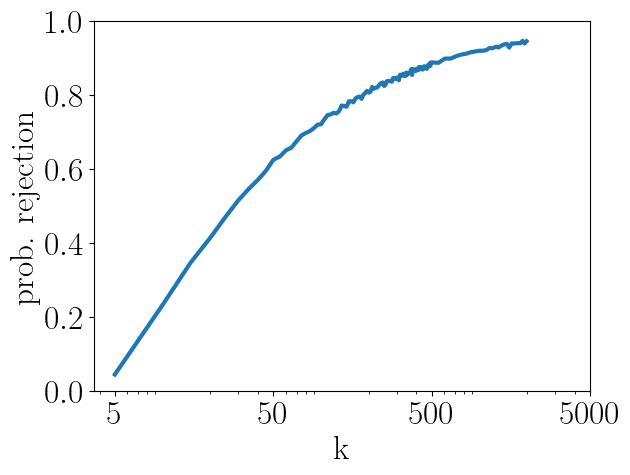
\includegraphics[width=.48\textwidth]{pics/failProbPlotMultinom.png}}
	\CaptionMargin
	\caption{Experiments on data generated by a simulation, showing the need for multiple tests correction.
		%
		The data has two protected groups, rankings are created by a multinomial process (``rolling a 3-sided dice'') with $p_G = (0.33, 0.33)$.
		%
		These rankings should have been rejected as unfair at a rate $\alpha = 0.1$.
		%
		However, we see that the rejection probability increases with $k$.
		%
		Note the scale of $k$ is logarithmic.}
	\label{fig:why-adjustment-is-needed-multinomial}
\end{figure}

Figure~\ref{fig:why-adjustment-is-needed-multinomial} illustrates what happens if we do not perform the correction.
%
In the figure, we assume there are two protected groups with $p_1=p_2=\frac{1}{3}$, and we perform simulations generating rankings of various lengths from $k=5$ to $k=5,000$.
%
For each value of $k$, we generate a set of rankings and perform $k$ tests with significance $\alphaadj=0.1$ for all of the prefixes of each ranking.
%
Then, we plot the probability of a Type-I error (declaring this fair ranking as unfair), and observe it is higher than $\alpha = 0.1$.
%

Our objective in this case would be to ensure that the overall rejection rate of fair rankings is $\alpha$.
%
If each of the $k$ tests performed on a ranking were independent, we could use {\v S}id{\'a}k's correction, and set $\alphaadj = 1 - (1 - \alpha)^{1/k}$.
%
However, the tests are not independent, as the tests with prefixes $k_1, k_2$ (for instance), overlap on their first $\min(k_1, k_2)$ elements.
%

\subsection{General Procedure}
\label{subsec:general-process}
%
With the presence of more than one protected group, the analytical extension of the model adjustment to a multinomial setting is too complex to be written into a closed formula.
%
In contrast to the model adjustment for one protected group which we used in~\cite{zehlike2017fair} (see also Section~\ref{sec:adjustment-binomial}), we found no analytical way to calculate all permutations which pass or fail the test.
%
Therefore we develop an experimental procedure to adjust $ \alpha $:
%
\begin{enumerate}
	\item Get input $ p_G, k, \alpha $.
	\item Build mTree with input $ \alpha $.
	\item Create $M$ rankings by rolling a biased $ |G| $-sided dice with each side's probability to show corresponding to a minimum proportion in vector $ p_G $.
	\item Test all those rankings against the mTree and count how many tests fail.
	%
	Remember that we want to observe a maximum failure probability of $ \failprob=\alpha $, because all rankings created by this multinomial stochastic process are considered to be inherently fair.
	\item If $ \failprob \neq \alpha $, we choose a new $ \alphaadj $ using a binary search heuristic.
	\item Now we build a new mTree using $ \alphaadj $ and repeat the procedure until $ \failprob \approx \alpha $.
\end{enumerate}
%
Once we found $\alphaadj$ we can recompute the mTrees from Figures~\ref{fig:mtree-symmetric-unadjusted} and~\ref{fig:mtree-asymmetric-unadjusted} to obtain an overall significance level of $\alpha = 0.1$.
%
Figures~\ref{fig:mtree-symmetric-adjusted} and~\ref{fig:mtree-asymmetric-adjusted} show the adjusted mTrees with the same parameters $p_G$.
\begin{figure}[h]
	\centering
	\begin{forest}
		for tree={
			child anchor=west,
			parent anchor=east,
			grow'=east,
			draw,
			anchor=west,
		}
		[{[0, 0]}
		[{[0, 0]}
		[{[0, 0]}
		[{[0, 0]} 
		[{[0, 0]}
			[{[1, 0]}
			[{[1, 0]}
				[{[2, 0]}
				[{[2, 0]}
					[{[3, 0]}]
					[{[2, 1]}]
				]]
				[{[1, 1]}, name=doubled1
				[{[1, 1]}
				[{[1, 1]}
				]]]
			]]
			[{[0, 1]}
			[{[0, 1]}, name=parentDoubled1
				[{[0, 2]}
				[{[0, 2]}
					[{[1, 2]}]
					[{[0, 3]}]
				]]
			]]
		]]]]]]
		\draw (parentDoubled1.east)--(doubled1.west);
	\end{forest}
	\CaptionMargin
	\caption{Example of an mTree with two protected groups with minimum proportions $ p_G=[1/3, 1/3] $ and $ \alphaadj=0.1 $. Compared to figure~\ref{fig:mtree-symmetric-unadjusted} this tree is less strict such that its \emph{total} probability $ \alphaadj $ of rejecting a fair ranking (i.e. a type-1-error) is 0.1.
	\label{fig:mtree-symmetric-adjusted}}
	\tablemargin
\end{figure}

\begin{figure}[h]
	\centering
	\begin{forest}
		for tree={
			child anchor=west,
			parent anchor=east,
			grow'=east,
			draw,
			anchor=west,
		}
		[{[0, 0]}
			[{[0, 0]}
				[{[0, 0]}
					[{[1, 0]}
						[{[1, 0]}
							[{[2, 0]}
								[{[2, 1]}
									[{[2, 1]}, name=doubled2, before drawing tree={y-=1em}
										[{[2, 1]}, before drawing tree={y-=1em}
											[{[3, 1]}, before drawing tree={y-=1em}]
											[{[2, 2]}, before drawing tree={y-=1em}]
										]
									]
								]
							]
							[{[1, 1]}, name=doubled1
								[{[1, 1]}, name=parentDoubled2
									[{[1, 2]}, name=doubled3, before drawing tree={y-=1em}
										[{[1, 2]}, before drawing tree={y-=1em}
											[{[1, 2]}, before drawing tree={y-=1em}]
										]
									]
								]
							]
						]]							
					[{[0, 1]}
						[{[0, 1]}, name=parentDoubled1
							[{[0, 2]}
								[{[0, 2]}, name=parentDoubled3
									[{[0, 3]}, before drawing tree={y-=1em}
										[{[0, 3]}, before drawing tree={y-=1em}
											[{[1, 3]}, before drawing tree={y-=1em}]
											[{[0, 4]}, before drawing tree={y-=1em}]
										]
									]
								]
							]
						]]
					]]]
		\draw (parentDoubled1.east)--(doubled1.west);
		\draw (parentDoubled2.east)--(doubled2.west);
		\draw (parentDoubled3.east)--(doubled3.west);
	\end{forest}
	\CaptionMargin
	\caption{Example of an mTree with two protected groups with minimum proportions $ p_G=[0.2, 0.4] $ and a corrected $ \alpha_c=0.1 $. 
	%
	The tree is less strict than the mTree in Figure~\ref{fig:mtree-asymmetric-unadjusted}.
	%
	The adjusted tree yields an overall false-negative rate of $ \alpha_c=0.1 $ when testing rankings for ranked group fairness.
	\label{fig:mtree-asymmetric-adjusted}}
	\tablemargin
\end{figure}

\subsection{Optimizations for the MTree Calculation}
\label{subsec:mtree-optimization}
In this subsection we explain how we optimize the adjustment procedure to reduce complexity, as it requires to compute a new mTree at each iteration which is expensive on its own.
%
Furthermore, depending on the level of accuracy needed, a large number of iterations $M$ might be required and the binary search heuristic may need many steps to find $\alpha$, if large intervals have to be searched.
%
We use three strategies to drastically reduce computational costs of this simulation-based adjustment:
%
\begin{inparaenum}[(i)]
%
\item we reduce the space requirements of the mTree structure;
%
\item we exploit the monotonicity of $\alphaadj$ with respect to $\alpha$ and use a regression procedure to speed up the binary search.
%
\item we apply the adjustment procedure for small trees first and only increase $k$, if we found the correct  $\alphaadj$ for the small trees.
\end{inparaenum}

\subsubsection{Reducing mTree Space Requirements.}
\label{subsubsec:reducing-space-requirements}
We improve the mTree data structure by excluding the calculation and storage of redundant information.
%
First we store each node only once at each level and duplicate nodes are combined into a single node with multiple parents.

Second, in case of equal minimum proportions for all groups $p_1 = p_2 = \ldots = p_{|G|}$ the mTree shows a convenient property that we can use to reduce additional space, as well as computation time.
%
Remember that whenever the multinomial CDF value falls below $\alpha$ for a particular position $i$, we have to put a protected candidate onto $i$.
%
For equal minimum proportions the tree branches into $|G| - 1$ symmetric nodes $m(i)$ of the same likelihood.
%
As an example reconsider the mTree from Figure~\ref{fig:mtree-symmetric-adjusted} at level 6.
%
For two protected groups with minimum proportions $[1/3, 1/3]$ we see that the tree branches into two symmetric nodes $[1, 0]$ and $[0,1]$.
%
Both have the same multinomial CDF values.
%
We store only one of the nodes and flag it as ``has mirrored node'' and continue our mTree computation only in the stored branch.
%
This way we save half of the space and computation time needed, without loosing any information about the tree.

Furthermore we reduce the size of the mTree by actually leaving out the parent-child relationship and merely storing the nodes itself together with their respective depth levels.
%
Figures~\ref{fig:mtree-symmetric-adjusted} and~\ref{fig:mtree-asymmetric-adjusted} show the mTree structure with all parent-child relations as edges.
%
We leave out these edges, thus reducing space, because we can prove that, if a single node exists on each level, which accepts a given ranking as fair, then a valid path to that node exists in the tree.

Before we can prove this property, we need to introduce the following definition, which formalizes what a successful mTree test at level $i$ looks like.
%
\begin{definition}[Successful mTree Testing]
\label{def:valid-mtree-test}
Let $\tau$ be a ranking of size $k$ and $\tau_{G,i}=(\tau_{1},\ldots,\tau_{|G|})$ the numbers of ranked protected elements from group $1,\ldots,|G|$ up to position $i$.
%
Let furthermore $MT$ be a $mTree$, with $MT_{G,i}=[m_1(i),\ldots,m_{|G|}(i)]$ the number of protected candidates of group $1,\ldots,|G|$ required up to position $i$.
%
We write $\tau_{G,i} \geq m_{G,i}$ if $\tau_g \geq m_g$ for all $g=1,\ldots,|G|$.
%
We call a test on level $i$ of $MT$ successful, iff $\tau_{G,i} \geq m_{G,i}$.
\end{definition}
%
Again, in order to remove the parental relationships in the mTree, thus reducing storage space, we have to prove that, if we test a ranking on each level of the mTree successfully, the entire ranking will be fair according to the ranked group fairness definition.
%
We prove this by showing that, if a ranking passes the test for any two nodes $n_1$ and $n_2$ at two consecutive levels $h$ and $h+1$, and $n_1$ is \emph{not} a parent of $n_2$, then all actual children of $n_1$ will have a weaker requirement than $n_2$ and will hence also test successfully.
%
Furthermore we show that all nodes at level $h+1$ for which the ranking fails the test are part of a path that already rejected it as unfair at level $h$.
%
Consider an example from Figure~\ref{fig:mtree-symmetric-adjusted} : Let us assume a ranking passes the test at level $9$ with exactly the required protected items $[1,1]$.
%
Now lets assume that at level $10$, the given ranking would pass the test for node $[2,1]$, which is not a successor of $[1,1]$.
%
In fact we see that the actual successor of $[1,1]$ is a node with the same configuration $[1,1]$.
%
However, if our ranking passes the test for the stricter node $[2,1]$, it also passes for $[1,1]$ and thus we do not need to know the true parent of $[2,1]$.
%
Note that the ranking would fail at node $[3,0]$, but with $[1,1]$ at level 9 it would have failed already at $[3,0]$'s predecessor $[2,0]$.
%
\begin{theorem}
\label{theorem:lazy-mTree-test}
Let $MT$ be a mTree and $\tau$ a ranking of size $k$.
%
There exists at least one successful test for $\tau$ at each level of $MT$,
iff there exists a valid path from the root of $MT$ to a leaf of $MT$.
\end{theorem}
%
\begin{proof}
	\label{proof:lazy-mTree-test}
	It is clear that at least one successful test per level is necessary for the path to exist.
	%
	Let us proof that one successful test is a sufficient condition for the path to exist.
	%
	Let $MT$ be a mTree and $\tau$ be a ranking that passes the test at level $h$ of $MT$.
	%
	Let $m_{G,h}=[m_{1}(h), \ldots, m_{|G|}(h)]$ be the node on level $h$ that successfully tested $\tau$.
	%
	Let further be $\tau_g(h)$ the number of protected candidates of group $g$ ranked at up to position $h$.
	%
	Without loss of generality let $\sum_{g=1}^{|G|} |m_{g}(h) - \tau_{g}(h)| = 0$, meaning that the ranking includes the exact amount of required protected candidates at level $h$ and not more.
	%
	Let $m_{G,(h+1)}$ be a node which tests $\tau$ successfully on level $h+1$ with $\sum_{g=1}^{|G|} |m_{g}(h+1) - \tau_{g}(h+1)| = 0$.
	%
	For all entries $m_{g}(h+1)$ of $m_{G,(h+1)}$ it is that $m_{g}(h) \leq m_{g}(h+1)$ by construction of the mTree, in which requirements for protected candidates can only increase or stay the same, but cannot decrease.

	\noindent We can now distinguish between the following two cases:
	\\
	\textbf{Case 1:} $m_{G,(h+1)}$ is a child of $m_{G,h}$.
	%
	Then they form a path. %UNNECESSARY:% Note that $\sum_{g=1}^{|G|} (m_{g}(h+1) - m_{g}(h) \leq 1)$.
	\\
	\textbf{Case 2:} $m_{G,(h+1)}$ is not a child of $m_{G,h}$.
	%
	Let now ${m'}_{G,(h+1)}$ be a child of $m_{G,(h)}$.
	%
	Because of $\sum_{g=1}^{|G|} |m_{g}(h) - \tau_{g}(h)| = 0$, and a successful test at level $h+1$, the following inequations hold: $\sum_{g=1}^{|G|} |m_{g}(h) - m_g(h+1)| \leq 1$ and $\sum_{g=1}^{|G|} |m_{g}(h) - m'_g(h+1)| \leq 1$.
	%
	If $\sum_{g=1}^{|G|} |m_{g}(h) - m_g(h+1)| = \sum_{g=1}^{|G|} |m_{g}(h) - m'_g(h+1)| = 0$ or $\sum_{g=1}^{|G|} |m_{g}(h) - m_g(h+1)| = \sum_{g=1}^{|G|} |m_{g}(h) - m'_g(h+1)| = 1$, it follows that $m_{G,(h+1)} = {m'}_{G,(h+1)}$ and we would have a contradiction with the fact that ${m'}_{G,(h+1)}$ is not a child of $m_{G,h}$, because then the nodes would be equal or different by one unit in one position.

	Hence, we need that either
	(2.1) $\sum_{g=1}^{|G|} |m_{g}(h) - m_g(h+1)| = 1$ and $\sum_{g=1}^{|G|} |m_{g}(h) - m'_g(h+1)| = 0$,
	or
	(2.2) $\sum_{g=1}^{|G|} |m_{g}(h) - m_g(h+1)| = 0$ and $\sum_{g=1}^{|G|} |m_{g}(h) - m'_g(h+1)| = 1$.
	%
	Case (2.1) means because of $\sum_{g=1}^{|G|} |m_{g}(h) - m_g(h+1)| = 1 < \sum_{g=1}^{|G|} |m_{g}(h) - m'_g(h+1)| = 0$ that the mTree accepts a ranking with one more protected candidate than required by the actual child of $m_{G,h}$, which contradicts our hypothesis that the ranking included the exact amount of required protected candidates. It follows that if we test $\tau_g (h+1)$ successfully with $m_{G,h+1}$ it would also satisfy ${m'}_{G,h+1}$.
Case (2.2) is impossible according to algorithm \ref{alg:imcdf}.
In detail, if $\sum_{g=1}^{|G|} |m_{g}(h) - m_g(h+1)| = 0$ it means that $ m_g(h+1) = m_{g}(h)$ and therefore, $F(m_{g}(h);h+1,p_G) > \alpha$ (line $4$ of algorithm \ref{alg:imcdf}). But if for the child of $m_{G,h}$, namely ${m'}_{G,h+1}$ it holds that $\sum_{g=1}^{|G|} |m_{g}(h) - m'_g(h+1)| = 1$, it means that
$F(m_{g}(h);h+1,p_G) \leq \alpha$ so that we would have added a new node as a child of $m_{g}(h)$ according to lines  $8-14$ of algorithm \ref{alg:imcdf}. Since both conditions cannot be true at the same time, Case (2.2) can not occur.
\\
In summary, Case (2.1) will only occur if we ranked more protected candidates than needed, and that the resulting test would be more strict than following a path through the mTree.
%
We showed that Case (2.2) is impossible. There is only Case 1 left if we have ranked exactly the number of protected candidates needed at each level of the mTree.
%
It follows that for any ranking that is tested successfully on each level of the mTree, it either was tested by nodes of a path through the mTree or was tested by a series of nodes which is more strict than such path.
\end{proof}
%
\noindent Because of Theorem~\ref{theorem:lazy-mTree-test} we do not need to keep the tree structure (i.e. parental relationship between nodes) and may store only a set of nodes for each level, while removing duplicate entries.

%
\begin{figure}[t!]
	\centering
	%
	\subfloat[Training data $R$ for a regression model to predict a good candidate for $\alphaadj$. Each pair $(k_j, \alpha_{c_j})$ is computed for small $k$ using the procedure described in Subsection~\ref{subsec:general-process}. \label{fig:regression-training-data}]
	{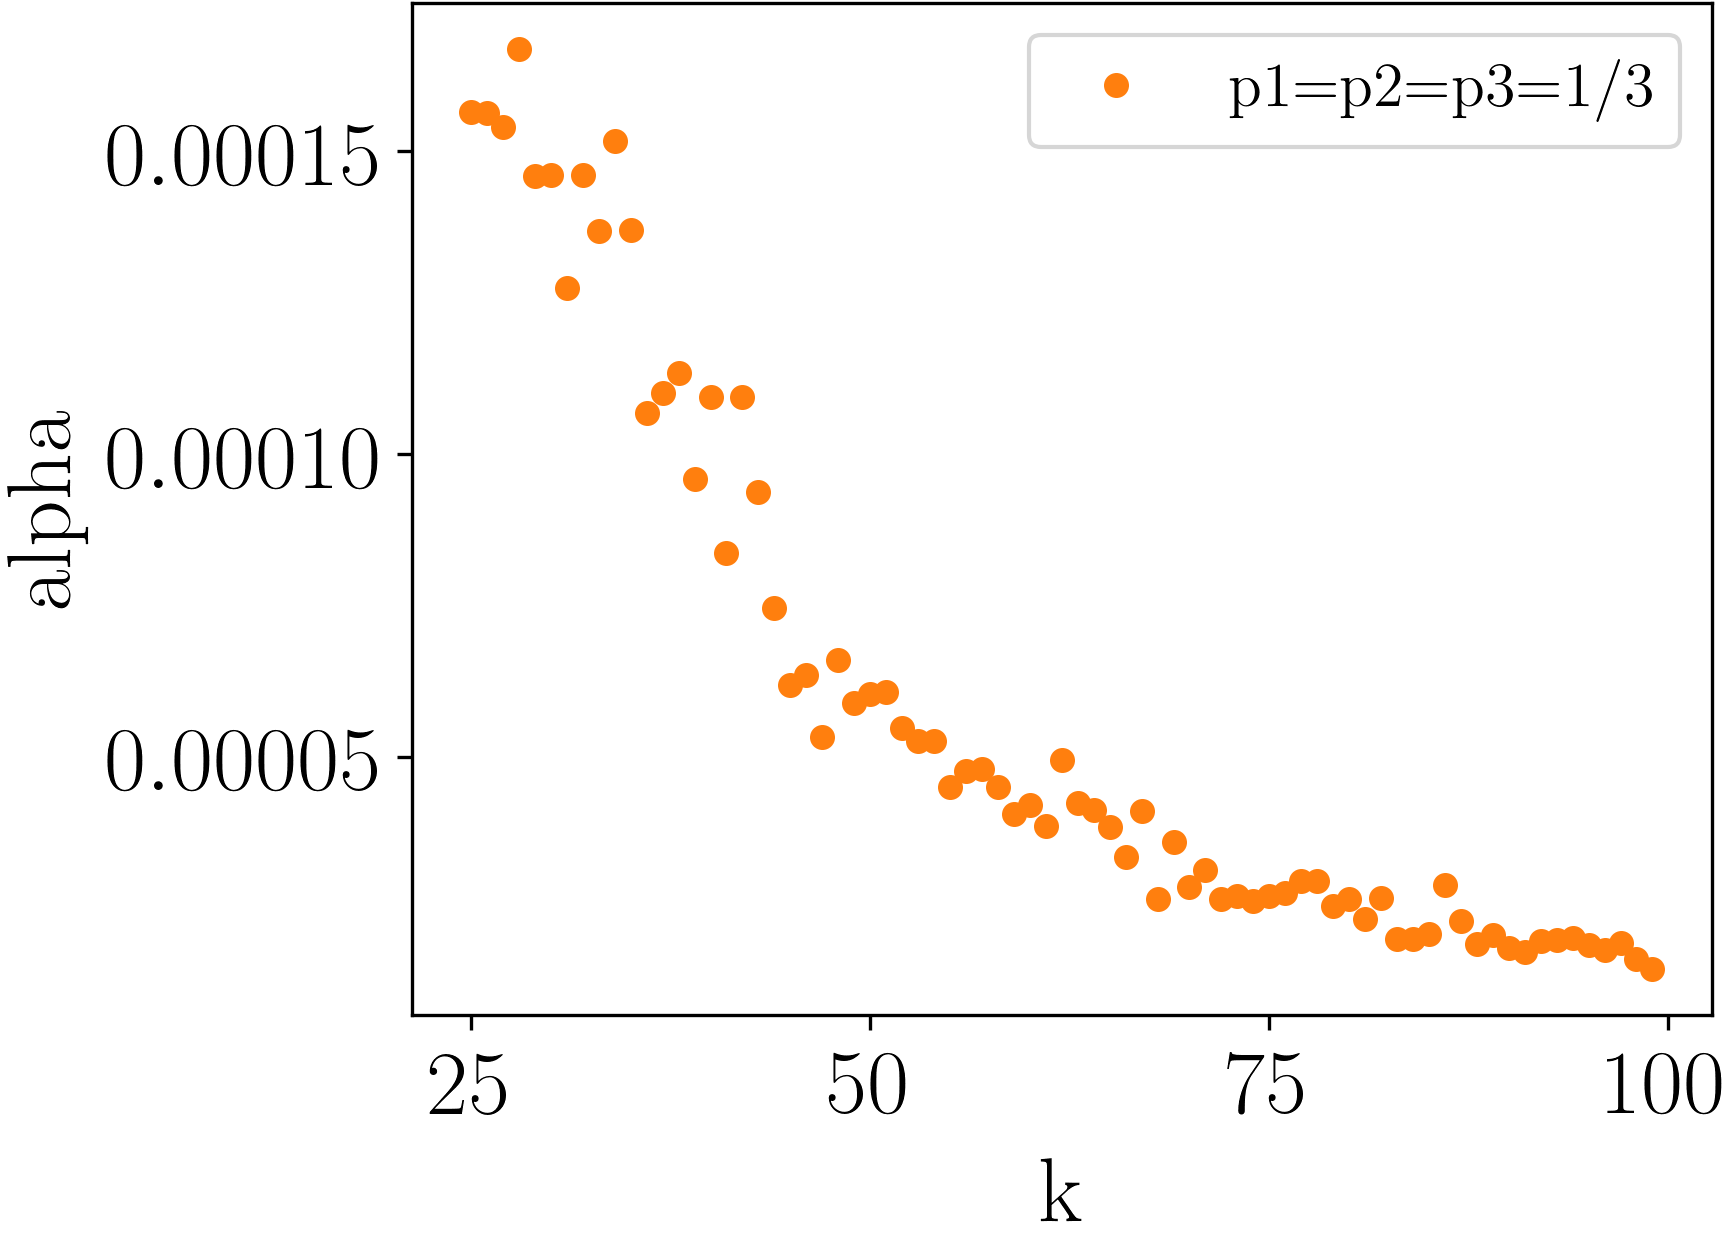
\includegraphics[width=.48\textwidth]{pics/alpha_030303_01.png}}\hfill
	%
	\subfloat[Computation time comparison between binary search only and binary search combined with regression for the multinomial significance adjustment.  \label{fig:regression-time-saved}]
	{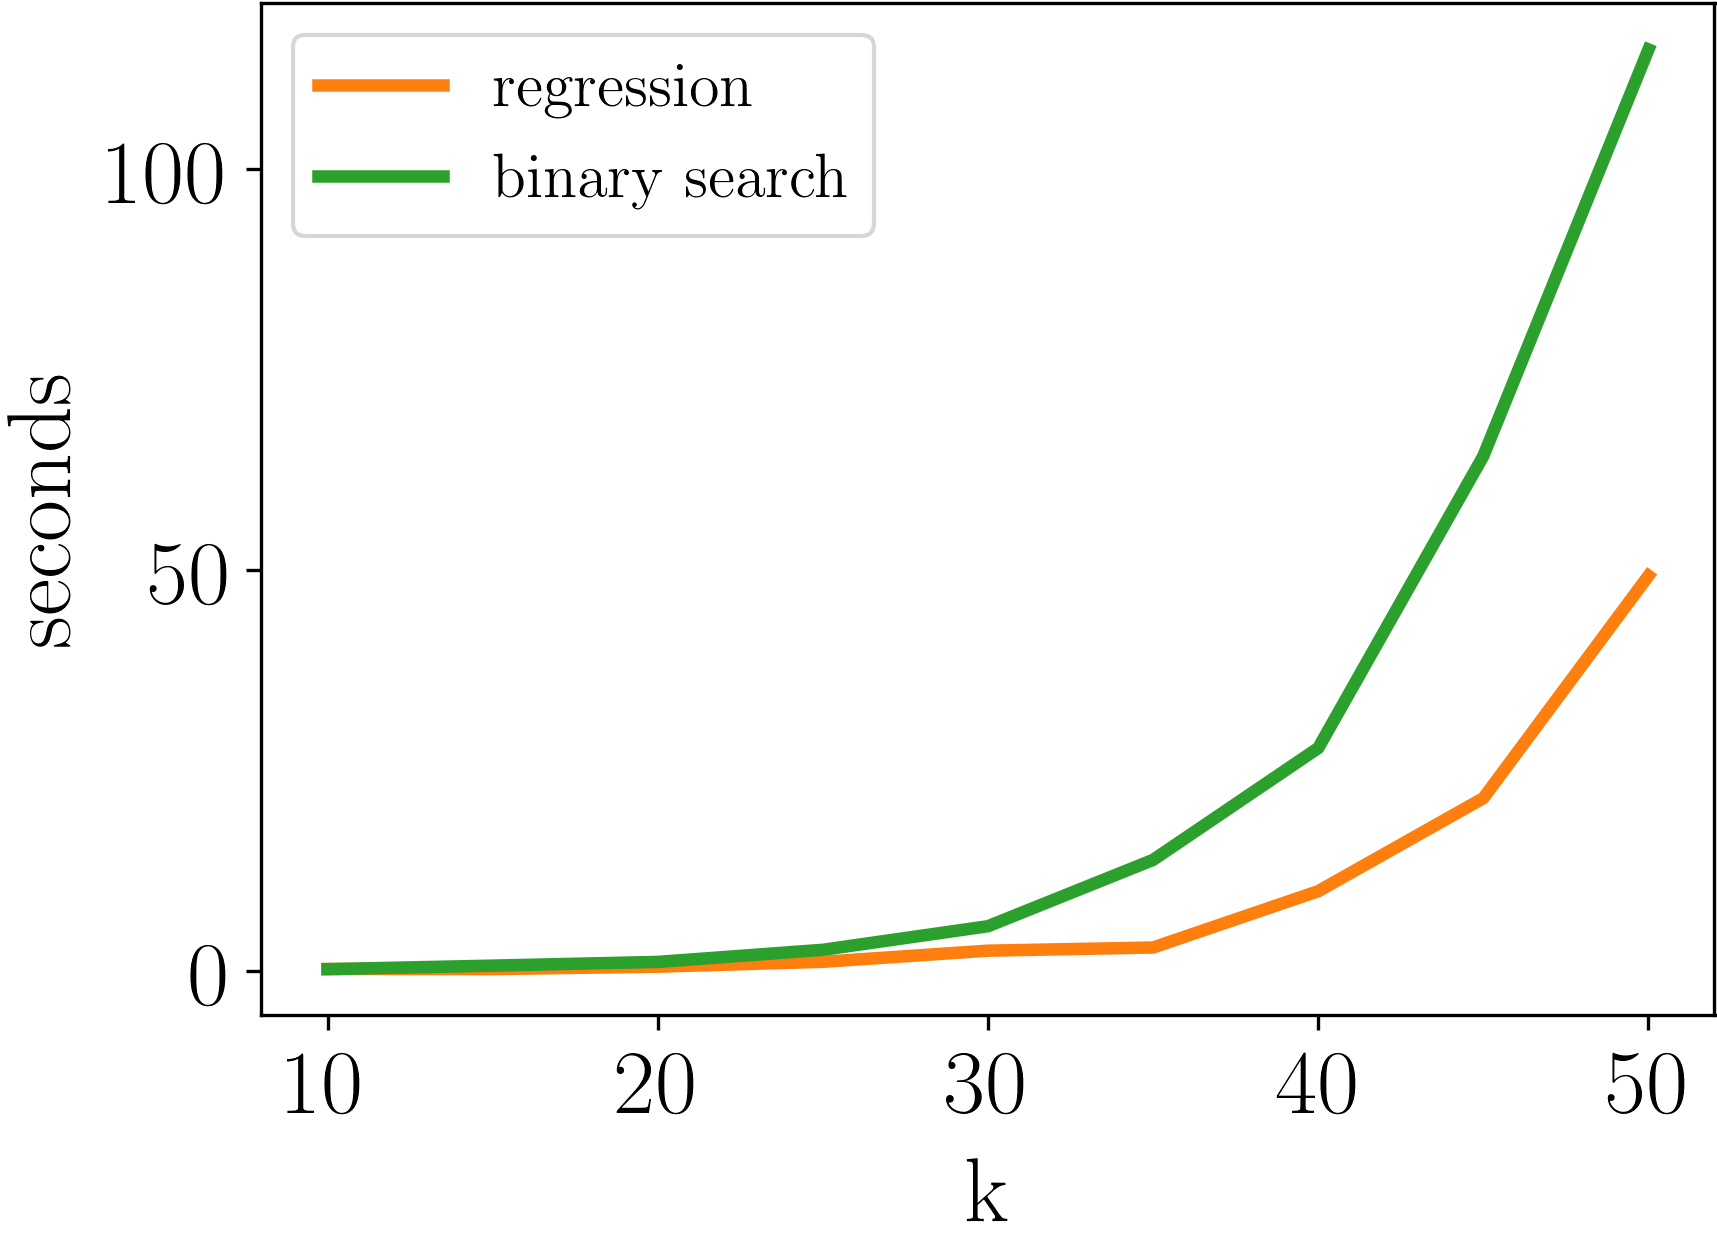
\includegraphics[width=.48\textwidth]{pics/computationTimeRegressionVSBinaryMultinomial.png}}\hfill
	\tablemargin
	\caption{}
	\label{fig:regression_adjustment_benefits}
\end{figure}
\subsubsection{Finding a Good Starting Candidate for the Binary Search}
We use a second-degree polynomial regression model to get our first estimate for a good $\alphaadj$ candidate and apply the binary search heuristic from that candidate, rather than starting with a random value, that might be very far away from the correct $\alphaadj$.
%
We need a few additional parameters as input: \texttt{kTarget} -- the length of the target ranking, \texttt{kStart} -- the size of the first mTree, \texttt{maxPreAdjustK} -- the maximum size of the mTree before we use regression to predict a good candidate $\alpha_{c_r}$ for the final $\alphaadj$, and \texttt{num\_iterations} -- the number of training instances to be computed.
%
To create a training dataset $R$, we compute \texttt{num\_iterations} small mTrees (i.e. with different $k \leq $ \texttt{maxPreAdjustK}) and adjust the respective $\alpha$ values as described in Subsection~\ref{subsec:general-process}.
%
For each iteration $j$ the pair $(k_j, \alpha_{c_j})$ is stored as a training instance in $R$.
%
Figure~\ref{fig:regression-training-data} shows a training set for $p_G=[1/3, 1/3], \texttt{maxPreAdjustK}=100$.
%
Then a regression model is trained to predict $\alpha_{c_r}$ for \texttt{kTarget}.
%
This $\alpha_{c_r}$ is now used to start the binary search for the correct and final $\alphaadj$.
%
Figure~\ref{fig:regression-time-saved} shows the runtime difference for the model adjustment routine with and without the use of regression.

\subsubsection{Adjusting for Small $k$ First}
We use the fact that given a value of $\alpha$, the mTree calculation is not dependent on $ k $, i.e., a mTree for $k=20$ and a mTree for $k=10$ for the same $\alpha$ are equal in the first ten positions.
%
This means that we can start the adjustment from the root node and expand the tree gradually to find the correct $ \alphaadj $, because if $\failprob$ is too high for given $k$, it will also be too high for any $k' > k$. %in particular and we do not have to consider the larger tree, as long as we do not have a good $\alphaadj$ for $k=10$.
%
%In order to show that we can indeed do that, assume that the for loop of algorithm \ref{alg:computeMTree} stops at $k=10$ instead of $k=20$.
%
%Furthermore, we can understand the mTree as a set of rules that a ranking has to satisfy.
%
%If there are no rules for how many protected candidates are required after position $10$, this is equivalent to not requiring more protected candidates after position $10$.
%
%Thus, the probability that a fair ranking is rejected by a shorter mTree is less or equal to a deeper mTree.
%
%We utilize this property to lower computational costs: we calculate the mTree for $k=10$, then create 10000 rankings of length 10 and calculate $ \alphaadj $ under this setting.
%
%Then we set $ k=k+ $\texttt{stepsize}, and repeat the procedure until we reach the desired ranking length.
%
We can see in Figure~\ref{fig:why-adjustment-is-needed-multinomial} that $ \failprob $ grows very fast for small $k$, which makes an early adjustment of $\alpha$ most efficient to save computation time.
%
%Figure~\ref{fig:regression-time-saved} shows the reduction of computation time when we combine the binary search with a regression and the pre-adjustment strategy.

\subsection{Final Adjustment Algorithm}
Algorithm~\ref{alg:regression_search} shows the overall adjustment algorithm in pseudo-code, which performs the following steps:
%
\begin{enumerate}
	\item Define the necessary parameters: \texttt{kTarget}, \texttt{kStart}, \texttt{maxPreAdjustK}, and \texttt{num\_iterations}
	\item Adjust $\alpha$ for a mTree of size \texttt{kStart} to get $\alpha_{c_1}$ using binary search.
	\item Add pair $\left(\texttt{kStart}, \alpha_{c_1}\right)$ to a regression training set $R$.
	\item \label{stepBegin} Increase $\texttt{kStart}$ by $\texttt{stepsize}=\frac{\texttt{maxPreAdjustK}}{\texttt{num\_iterations}}$
	\item Compute a mTree with parameters $\texttt{kTarget}, p_G, \alpha_{c_1}$ and adjust $\alpha_{c_1}$.
	\item \label{stepEnd} Name result $\alpha_{c_2}$ and add pair $\left(\texttt{kStart}, \alpha_{c_2}\right)$ to $R$.
	\item Repeat steps (\ref{stepBegin}) -- (\ref{stepEnd}) until $\texttt{kStart} == \texttt{maxPreAdjustK}$.
	\item Train a regression model with training data $R$ to predict $\alpha_{c_r}$ for $\texttt{kTarget}$.
	\item Use binary search (Algorithm~\ref{alg:mult_binary}) to find $\alphaadj$ for parameters $k,p_G, \alpha_{c_r}$.
\end{enumerate}
%
\begin{algorithm}[t!]
	\caption{Algorithm \algoReg estimates the corrected significance level $\alphaadj$ such that the mTree $m(\alphaadj , k, p_G)$ has the probability of rejecting a fair ranking $\alpha$}
	\label{alg:regression_search} % But whenever possible refer to this algo. by name not number
	\small
	\AlgInput{\texttt{kStart} -- depth of the mTree to start with; $k$ -- the length of the ranking; $p_G$ -- the desired proportions of the protected groups; $\alpha$ -- the desired significance level;  \texttt{maxPreAdjustK} the maximum depth of the mTrees that are used as training data; \texttt{num\_iterations} -- the number of steps between \texttt{kStart} and \texttt{maxPreAdjustK}}
	\AlgOutput{$\alphaadj$ -- the adjusted significance}
	$R \leftarrow \lbrace \rbrace; \alpha_{\textit{new}} \leftarrow \alpha$	\\
	\AlgComment{divide the interval [$\text{kStart}, \text{maxPreAdjustK}$] into num\_iterations parts}
	$\texttt{stepsize} \leftarrow \max(\frac{\texttt{maxPreAdjustK}}{\texttt{num\_iterations}}, 1)$ \\
	\For{$i\leftarrow 0$ to $\texttt{num\_iterations}$}{
		\AlgComment{adjust $\alpha_{\text{new}}$ for the current kStart}
    	$\alpha_{\text{new}} \leftarrow \textsc{MultinomialBinarySearchAdjustment}(\alpha_{\textit{new}}, \texttt{kStart}, p_G)$ \\
    	\AlgComment{add the pair (kStart, $\alpha_{\textit{new}}$) to the training data $R$}
    	$R.\textit{put}(\texttt{kStart},\alpha_{\textit{new}})$ \\
    	\If{$\texttt{kStart} + \texttt{stepsize} \leq \texttt{maxPreAdjustK}$}{
    		$\texttt{kStart} \leftarrow \texttt{kStart} + \texttt{stepsize}$ \\
    	}\Else{
			break
    	}
    }
    $\texttt{coeffs} \leftarrow R.\textit{train}()$ \AlgComment{returns the vector of predicted coefficients for the curve over $R$}
    $\alpha_{c_r} \leftarrow \texttt{coeffs[0]} + \texttt{coeffs[1]} * k + \texttt{coeffs[2]} * k^2$ \\
    $\alphaadj \leftarrow \textsc{MultinomialBinarySearchAdjustment}(\alpha_{c_r},k,p_G)$ \\
    \Return{$\alphaadj$}
\end{algorithm}

\subsection{Further Optimizations}
In addition to the optimizations \emph{during} mTree calculation which we presented in Subsection~\ref{subsec:mtree-optimization}, our implementation caches already computed mTrees and their components to never do the same computation twice.
%
We denote that a mTree has to be computed only once for a particular combination of $k, p_G, \alpha$.

\subsubsection{MCDF Cache}\label{subsubsec:mcdf-cache}
Table~\ref{tbl:time-space} shows that the highest computational cost arises from computing the multinomial cumulative distribution function $F$.
%
In the worst case Algorithm~\ref{alg:imcdf} computes it $|G|+1$ times for each group $g$ in $m_g(i)$ and each position $i\leq k$.
%
However, the same calculation may be done many times:
%
As an example consider the (fictive) mTree nodes $[2,1]$ and $[1,2]$ at position $k=3$.
%
To compute the successors of node $[2,1]$ we call Algorithm~\ref{alg:imcdf} with arguments $(4,[2,1])$, $(4,[3,1])$ and $(4,[2,2])$.
%
We store the results of these calculation in a map that we call MCDF cache with the algorithm arguments ($k$ and the minimum protected candidates of each group) as key and the corresponding mcdf as value.
%
Next we compute the successors of node $[1,2]$ and call Algorithm~\ref{alg:imcdf} with arguments $(4,[1,2])$, $(4,[2,2])$ and $(4,[1,3])$.
%
We see that we would compute the mcdf for $(4,[2,2])$ twice, but instead we can now read it from the MCDF cache.

%Furthermore, if our example has symmetric minimum proportions $p_1 = p_1$, the mcdf of $(4,[2,1])$ is equal to $(4,[1,2])$ and $\textit{mcdf}(4,[1,3]) = \textit{mcdf}(4,[3,1])$.
%%
%Generally, if $p_1 = p_2 = \cdots = p_{|G|}$, we can make use of the mTree's symmetry: we calculate the mcdf only for node $m(i)$ and store it in the cache \emph{as well as its mirror} (see Subsection~\ref{subsubsec:reducing-space-requirements}), because their mcdf values are the same.

Note that the mcdf computation is only depends on $p_G$ and not on $alpha$.
%
We can therefore persists the MCDF cache on disk for a particular vector $p_G$ and load it for any mTree calculation with the same $p_G$ in the future.

\subsubsection{Stored mTrees}
\label{subsubsec:stored-mtrees}
During the computation of an adjusted mTree with parameters $k,p_G , \alpha$ we calculate many temporary mTrees (first the unadjusted ones, then the ones for the regression algorithm, then the ones for the binary search steps).
%
We persist all of the temporary mTrees plus the final tree in files for later usage.
%
The filenames contain the tree parameters, whether or not it is adjusted, and its probability to fail a fair ranking $\failprob$.
%
If any of these trees is needed at a later point in time it can be loaded from disc instead of being recomputed, be it as input for multinomial \algoFAIR or as temporary tree during a new adjusted mTree computation.

\subsection{Complexity Analysis}
\begin{table}[t!]
	\tablemargin
	\caption{Time complexity for all algorithms without pre-computed results.\label{tbl:time-space}}
	\vspace{-4mm}
	\scalebox{0.75}{
		\begin{tabular}{lll}
			\toprule
			\textbf{Algorithm} & \textbf{Time Complexity} & \textbf{Space Complexity}\\
			\midrule
			\rowcolor[HTML]{C0C0C0}
			\algoImcdf & $\mathcal{O}(|G|) \cdot \mathcal{O}(\text{MCDF}(k,p,\alpha ))$ & $\mathcal{O}(|G|^2)$ \\
			\algoComputeMTree & $\mathcal{O}(|G|^{k}) \cdot \mathcal{O}(\text{\algoImcdf})$ & $\mathcal{O}(|G|^{k})$\\
			\rowcolor[HTML]{C0C0C0}
			\algoMultBinary & $\mathcal{O}(\log{}\frac{\alpha}{\epsilon}) \cdot (\mathcal{O}(k^2) + \mathcal{O}(\text{\algoComputeMTree}))$  & $\mathcal{O}(|G|^k)$\\
			\algoReg & $\mathcal{O}(\log{}\frac{\alpha}{\epsilon}) \cdot (\mathcal{O}(k^2) + \mathcal{O}(\text{\algoComputeMTree}))$ & $\mathcal{O}(|G|^k)$\\
			\rowcolor[HTML]{C0C0C0}
			\algoFAIR & $\mathcal{O}(n \log{} n) + \mathcal{O} (\text{\algoMultBinary}) + \mathcal{O}(k)$ & $\mathcal{O}(|G|^k + n + k)$ \\
			\bottomrule
		\end{tabular}
	}
\end{table}

This section presents time and space complexity analyses for all algorithms from this section.
%
Table~\ref{tbl:time-space} shows the asymptotic costs for each algorithm without any pre-computed data (i.e. no mTree exists and the MCDF cache is empty).
%
The complexity analysis for \algoFAIR is done in Subsection~\ref{subsec:FAIR-complexity}, but Table~\ref{tbl:time-space} already contains the summary, such that it shows time and space complexity for all algorithms in this paper.

\subsubsection{\algoImcdf complexity}\label{subsubsec:imcdf-complexity}
The complexity of the multinomial cdf is dependant on the current position $i$ (also understood as \textit{number of trials}), $|G|$ the number of protected groups, and $m_{G,i}$ the vector of minimum required protected candidates for each group at position $i$ (also \textit{number of successes}).
%
We will write $\mathcal{O}(\text{MCDF}(i,p_G,\alpha))$ as the asymptotic complexity of this function.
%
In the library we used for our implementation, the time complexity to calculate the multinomial CDF at position $i$ is in $\mathcal{O}(\text{MCDF}(i,p_G,\alpha)) = \mathcal{O}(i^{|G|})$.
%
Thus the most expensive position to calculate the multinomial CDF for is $k$.
%
For the overall time complexity of \algoImcdf we get $\mathcal{O}(|G|) \cdot \mathcal{O}(\text{MCDF}(k,p,\alpha ))$ with $|G|$ being the number of protected groups.
%
The space complexity is $\mathcal{O}(|G|^2)$ because we store $|G|$ nodes, with each node being an array of length $|G|$.
%
\subsubsection{\algoComputeMTree complexity}\label{subsubsec:mtree-complexity}
Algorithm \algoComputeMTree constructs an mTree of depth $k$.
%
There may be up to $|G|$ possible children for each node in the tree resulting in $|G|^{k-1} +1$ nodes, leading to a time complexity of $\mathcal{O}(|G|^{k}) \cdot \mathcal{O}(\text{\algoImcdf})$.
%
We store $|G|^{k-1} +1$ nodes with arrays of length $|G|$, leading to space complexity of $\mathcal{O}(|G|^{k})$.
%
\subsubsection{\algoMultBinary complexity}\label{subsubsec:multBinary-complexity}
Also in the multinomial case we adjust $\alpha$ to $\alpha_c$ with a binary search heuristic.
%
However there is no discrete measure for mTrees as was in case of the mTable mass.
%
Therefore the complexity of the binary search depends on the tolerance $\epsilon$ set beforehand as a stopping criteria.
%
As we are searching on the interval $\left[0,\alpha\right[$ the resulting number of possible mTrees is $\frac{\alpha}{\epsilon}$.
%
Thus the binary search needs $\mathcal{O}(\log{}\frac{\alpha}{\epsilon})$ time because we calculate one mTree and its fail probability for each step.
%
The fail probability is computed experimentally by creating 10.000 rankings and testing them against the current mTree.
%
This process needs $\mathcal{O}(10.000 \cdot k)$ to create the rankings plus $\mathcal{O}(k)$ to test each of them.
%
Hence the overall time complexity becomes $\mathcal{O}(\log{}\frac{\alpha}{\epsilon}) \cdot (\mathcal{O}(k^2) + \mathcal{O}(\text{\algoComputeMTree}))$.
%
The space complexity is in $\mathcal{O}(|G|^k)$ for storing three mTrees and their fail probability.
%
\subsubsection{\algoReg complexity}\label{subsubsec:regression-complexity}
Algorithm \algoReg has the same asymptotic complexity as \algoMultBinary.
%
However a significant reduction in computation time compared can be achieved when combining the two, instead of using \algoMultBinary only (see Figure~\ref{fig:regression_adjustment_benefits}, green vs. orange line).
\FloatBarrier

\section{Algorithm}\label{sec:algorithms}
We present the multinomial \algoFAIR algorithm (\S\ref{subsec:algorithm-description}) and prove it is correct (\S\ref{subsec:algorithm-correctness}).

\subsection{Algorithm Description}\label{subsec:algorithm-description}
\note{Done}
Multinomial \algoFAIR, presented in Algorithm~\ref{alg:fair}, solves the {\sc Fair Top-$k$ Ranking} problem for multinomial protected groups and intersectional group settings.
%
As input, multinomial \algoFAIR takes 
the expected size $k$ of the ranking to be returned,
the qualifications $q_c$, 
indicator variables $g_c$ indicating if candidate $c$ is protected,
the vector of minimum target proportions $p_G$, and
the adjusted significance level $\alphaadj$.

First, the algorithm uses $q_c$ to create priority queues with up to $k$ candidates each: $P_0$ for the non-protected candidates and $P_g$ for the protected candidates of group $g$.
%
Next (line \ref{alg:fair:mtree}), the algorithm derives a ranked group fairness tree (mTree) similar to Figure~\ref{fig:mtree-asymmetric-adjusted}, i.e., for each position it computes the minimum number of protected candidates per group, given $p_G$, $k$ and $\alphaadj$.
%
Then, multinomial \algoFAIR greedily constructs a ranking subject to candidate qualifications, and minimum protected elements required.
%
Note that the right choice of a tree node on level $i$ depends on the path chosen along the tree and therefore on its concrete parent at level $i-1$. 
%
In case \texttt{mtree} branches into different possibilities to satisfy ranked group fairness (as an example see Fig.~\ref{fig:mtree-asymmetric-adjusted} for $k=4$), the algorithm chooses the branch that has a higher value for $F$, meaning it chooses the branch that has a higher probability.
%
If two branches are equally likely, which happens for $p_1 = p_2 = \ldots = p_{|G|}$, then one of them is chosen at random.
%
Given this the algorithm has to find the correct child $m_{G,i}$ for a given parent from the previous level (Line~\ref{alg:fair:childNode}).
%
If the node demands a protected candidate from group $g$ at the current position $i$, the algorithm appends the best candidate from $P_g$ to the ranking (Lines \ref{alg:fair:pstart}-\ref{alg:fair:pend}); otherwise, it appends the best candidate from $P_0 \cup P_1 \cup \ldots \cup P_{|G|}$ (Lines \ref{alg:fair:anystart}-\ref{alg:fair:anyend}).
%

\begin{algorithm}[h]
	%\caption{Algorithm \algoFAIR, finding a ranking that maximizes utility subject to in-group monotonicity and ranked group fairness constraints.}
	\caption{Algorithm \algoFAIR finds a ranking that maximizes utility subject to in-group monotonicity and ranked group fairness constraints. Checks for special cases (e.g., insufficient candidates of a class) are not included for clarity.}
	\label{alg:fair}  % But whenever possible refer to this algo. by name not number
	\small
	\AlgInput{$k \in [n]$, the size of the list to return; $\forall~c \in [n]$: $q_c$, the qualifications for candidate $c$, and $g_c$ an indicator that is $>0$ iff candidate $c$ is protected; $p_G$ with $\forall p \in p_G \in ]0,1[$, the vector of minimum proportions for each group of protected elements; $\alphaadj \in ]0,1[$, the adjusted significance for each fair representation test.}
	\AlgOutput{$\tau$ satisfying the group fairness condition with parameters $p, \sigma$, and maximizing utility.}
	%\AlgComment{compute min. protected candidates per position}
	$P_0, P_1, \ldots P_{|G|} \leftarrow$ empty priority queues with bounded capacity $k$\\
	\For{$c \leftarrow 1$ \KwTo $n$}{
		insert $c$ with value $q_c$ in priority queue $P_{g_c}$ \\
	}

	$\texttt{mtree}(i) \leftarrow \texttt{\algoComputeMTree}(k, p_G, \alphaadj)$  \label{alg:fair:mtree}\\
		
	%\AlgComment{create fair ranking}
	$(t_0, t_1, \ldots, t_{|G|}) \leftarrow (0, \ldots, 0)$ \\
	$i \leftarrow 0 $ \\
	\While{$i < k$}{
		\texttt{noCandidateAdded = True} \\
		\AlgComment{get next node in tree path}
		$m_{G, i} = [m_1(i), \ldots, m_{|G|}(i)] \leftarrow \texttt{findNextNode(mtree, i)}$ \label{alg:fair:childNode}\\
		\AlgComment{find which group needs a new candidate}
		\For{\texttt{g = 1; g} $\leq$ \texttt{|G|; g++}}{

			\If{$t_g < m_g(i)$}{\label{alg:fair:pstart}
				\AlgComment{add a protected candidate}
				$t_g \leftarrow t_g + 1$ \\ 
				$\tau[i] \leftarrow \operatorname{pop}(P_g)$ \\  
				\texttt{noCandidateAdded = False}
			}\label{alg:fair:pend}
		}
		\If{\texttt{noCandidateAdded}}{ \label{alg:fair:anystart}
			\AlgComment{no protected candidate needed: add the best available}
			$P_g \leftarrow$ \texttt{findBestCandidateQueue()} \\
			$\tau[i] \leftarrow \operatorname{pop}(P_g)$\\
			$t_g \leftarrow t_g + 1$ 
		}\label{alg:fair:anyend}
		
	}
	\Return{$\tau$}
\end{algorithm}
\vspace{-3mm}

\subsection{Algorithm Complexity}
\todo{Not done yet}

\begin{table}[]
\caption{Space and time complexity for all algorithms.
		\label{tbl:space_time}}
\begin{tabular}{|c|c|c|}
\hline
\textbf{Algorithm} & \textbf{Time Complexity} & \textbf{Space Complexity} \\ \hline
inverseBinomialCDF & $\mathcal{O}(n\log{}n)$ & $\mathcal{O}(n\log{}n)$ \\ \hline
\algoMtable & $\mathcal{O}(n\log{}n)$ & $\mathcal{O}(n\log{}n)$ \\ \hline
\algoRecursive & $\mathcal{O}(n\log{}n)$ & $\mathcal{O}(n\log{}n)$ \\ \hline
\algoBinomBinary & $\mathcal{O}(n\log{}n)$ & $\mathcal{O}(n\log{}n)$ \\ \hline
multinomialCDF & $\mathcal{O}(n\log{}n)$ & $\mathcal{O}(n\log{}n)$ \\ \hline
\algoImcdf & $\mathcal{O}(n\log{}n)$ & $\mathcal{O}(n\log{}n)$ \\ \hline
\algoComputeMTree & $\mathcal{O}(n\log{}n)$ & $\mathcal{O}(n\log{}n)$ \\ \hline
\algoMultBinary & $\mathcal{O}(n\log{}n)$ & $\mathcal{O}(n\log{}n)$ \\ \hline
\algoReg & $\mathcal{O}(n\log{}n)$ & $\mathcal{O}(n\log{}n)$ \\ \hline
\algoFAIR & $\mathcal{O}(n\log{}n)$ & $\mathcal{O}(n\log{}n)$ \\ \hline
\end{tabular}
\end{table}

\algoFAIR has running time $O(n + k \log k)$; which includes building the $O(k)$ size priority queues from $n$ items and processing them to obtain the final ranking, where we assume $k < O(n/\log n)$. 
\meike{Was soll denn $k < O(n/\log n)$ heißen? Warum ist die size der priority queues O(k) und nicht k?}
%
If we already have ranked lists for all groups of elements, \algoFAIR can avoid the first step and obtain the top-$k$ in $O(k \log k)$ time.
%
Our method is applicable as long as there is at least one protected group and there are enough candidates in each protected group; if there are $k$ from each group, the algorithm is guaranteed to succeed, otherwise the ``head'' of the ranking will satisfy the ranked group fairness constraint, but the ``tail'' of the ranking may not.

\subsection{Algorithm Optimizations}
\note{Done}
Because the computation of an adjusted mTree is expensive (Table~\ref{tbl:space_time}), our implementation persists already computed mTrees and their components to never do the same computation twice. 
%
Depending on the structure of $p_G$, different levels of optimization are applicable.

We note however that an mTree has to be computed only once for a particular combination of $k, p_G, \alpha$ and that \algoFAIR has a complexity of $O(k log k)$.
%
We provide the already pre-computed mTrees and MCDF caches for our experiments and the intermediate steps not only for reproducibility but for use in practice too.

\subsubsection{MCDF Cache}\label{subsubsec:mcdf-cache}
Table~\ref{tbl:space_time} shows that the highest computational cost arises from computing the multinomial cumulative distribution function $F$. 
%
In the worst case Algorithm~\ref{alg:imcdf} computes it $|G|+1$ times for each group $g$ in $m_g(i)$ and each position $i\leq k$.
%
However, the same calculation may be done many times:
%
As an example consider the (fictive) mTree nodes $[2,1]$ and $[1,2]$ at position $k=3$. 
%
To compute the successors of node $[2,1]$ we call Algorithm~\ref{alg:imcdf} with arguments $(4,[2,1])$, $(4,[3,1])$ and $(4,[2,2])$. 
%
We store the results of these calculation in a map that we call MCDF cache with the algorithm arguments ($k$ and the minimum protected candidates of each group) as key and the corresponding mcdf as value.
%
Next we compute the successors of node $[1,2]$ and call Algorithm~\ref{alg:imcdf} with arguments $(4,[1,2])$, $(4,[2,2])$ and $(4,[1,3])$. 
%
We see that we would compute the mcdf for $(4,[2,2])$ twice, but instead we can now read it from the MCDF cache.

Furthermore, if our example has symmetric minimum proportions $p_1 = p_1$, the mcdf of $(4,[2,1])$ is equal to $(4,[1,2])$ and $\textit{mcdf}(4,[1,3]) = \textit{mcdf}(4,[3,1])$. 
%
Generally, if $p_1 = p_2 = \cdots = p_{|G|}$, we can make use of the mTree's symmetry: we calculate the mcdf only for node $m(i)$ and store it in the cache \emph{as well as its mirror} (see Section~\ref{subsubsec:discarding-symmetric-nodes}), because their mcdf values are the same.

Note that the mcdf computation is only depends on $p_G$ and not on $alpha$. 
%
We can therefore persists the MCDF cache on disk for a particular vector $p_G$ and load it for any mTree calculation with the same $p_G$ in the future.
%
This also saves additional computation time during significance adjustment.

\subsubsection{Discarding symmetric nodes}
\label{subsubsec:discarding-symmetric-nodes}
In case of equal minimum proportions for all groups $p_1 = p_2 = \ldots = p_|G|$ the mTree shows a convenient property that we can use to reduce additional space and computation time. 
%
Remember that whenever the mcdf value falls below $\alpha$ for a particular position $i$, we have to put a protected candidate onto $i$. 
%
For equal minimum proportions the tree branches into $|G| - 1$ symmetric nodes $m(i)$ of the same likelyhood.
%
As an example reconsider the mTree from Figure~\ref{fig:mtree-symmetric-adjusted} at level 6. 
%
For two protected groups with minimum proportions $[1/3, 1/3]$ we see that the tree branches into two symmetric nodes $[1, 0]$ and $[0,1]$. 
%
Both have the same mcdf values.
%
We store only one of the nodes and flag it as ``has mirrored node'' and continue our mTree computation only in the stored branch.
%
This way we save half of the space and computation time needed, without loosing any information about the tree. 

\subsubsection{Stored mTrees}
\label{subsubsec:stored-mtrees}
During the computation of an adjusted mTree with parameters $k,p_G , \alpha$ we calculate many temporary mTrees (first the unadjusted ones, then the ones for the regression algorithm, then the ones for the binary search steps).
%
We persist all of the temporary mTrees plus the final tree in files for later usage.
%
The filenames contain the tree parameters and whether or not it is adjusted and its probability to fail a fair ranking $\failprob$.
%
If any of these trees is needed at a later point in time it can be loaded from disc instead of being recomputed, be it as input for multinomial \algoFAIR or as temporary tree during a new adjusted mTree computation.

\subsection{Finding the Optimal Ranking in Terms of Utility}\label{subsec:optimal-utility-extension}

By construction, a ranking $\tau$ generated by multinomial \algoFAIR satisfies in-group monotonicity, because all candidates are selected by decreasing qualifications.
%
It also satisfies the ranked group fairness constraint, because for every prefix of size $i$ the list, the number of protected candidates in group $g$ is at least $m_g(i)$. 
%
What we must prove is that $\tau$ achieves optimal selection utility, and that it maximizes ordering utility. 
%
This is done in the following lemmas.

\begin{lemma}\label{lemma:across}
	If a ranking satisfies the in-group monotonicity constraint, then the utility loss (ordering or selection utility different from zero) can only happen across groups, but not within.
\end{lemma}

\begin{proof}
	This comes directly from Definition~\ref{def:inGroupMonotonicity} given that for two candidates $c,d$, the only case in which $r(c,\tau) < r(d,\tau) \wedge q_c < q_d$ is when $g_c \ne g_d$.
\end{proof}

\begin{lemma}
	The optimal selection utility among rankings satisfying in-group monotonicity (\ref{problem:constraint-monotonicity}) and ranked group fairness (\ref{problem:constraint-rank}), is either zero, or is due to a non-protected candidate ranked below a less qualified protected candidate.
\end{lemma}

\begin{proof}
	Let $c,d$ be the two candidates that attain the optimal selection utility, with $c \in \tau, d \in [n] \backslash \tau$.
	%
	We will prove this by contradiction: let us assume $c$ is a non-protected candidate ($g_c=0$) and $d$ is a protected element ($g_d>0$). 
	%
	Let us swap $c$ and $d$, moving $c$ outside $\tau$ and $d$ inside the ranking, and then moving down $d$ if necessary to place it in the correct ordering among the protected elements below its position (given that $c$ is the last non-protected element in $\tau$). 
	%
	The new ranking continues to satisfy in-group monotonicity as well as ranked group fairness (as it has not decreased the number of protected elements at any position in the ranking), and has a larger selection utility. 
	%
	This is a contradiction because the selection utility was optimal. Hence, $c$ is a protected element and $d$ a non-protected element.
\end{proof}

\begin{lemma}\label{lemma:number-protected-implies-selfairness} %[Elements inside/outside a ranking are determined by $\tau_p$]
	Given two rankings $\rho, \tau$ satisfying in-group monotonicity (\ref{problem:constraint-monotonicity}), if for each protected group they have the same number of elements, i.e. $\rho_G = \tau_G$, then both rankings contain the same $k$ elements (possibly in different order), and hence both rankings have the same selection utility.
\end{lemma}

\begin{proof}
	Both rankings contain a prefix of size $\lVert\tau_G\rVert$ of protected candidates. 
	%
	Within each protected group candidates are ordered by decreasing qualifications.
	Also both rankings contain a prefix of size $k - \lVert\tau_G\rVert$ of non-protected candidates ordered by decreasing qualifications. 
	%
	Hence, $\forall c \in [n], c \in \tau \Leftrightarrow c \in \rho$, so the elements not included in the rankings are also the same elements, and the selection utility of both rankings is the same.
\end{proof}

The previous lemma means selection utility is determined by the number of protected candidates in a ranking.

\begin{lemma}\label{lemma:fair-optimal-selection}
	Algorithm \algoFAIR achieves optimal selection utility among rankings satisfying in-group monotonicity (\ref{problem:constraint-monotonicity}) and ranked group fairness (\ref{problem:constraint-rank}).
\end{lemma}

\begin{proof}
	Let $\tau$ be the ranking produced by \algoFAIR, and $\tau^*$ be the ranking achieving the optimal selection utility while satisfying constraints~(\ref{problem:constraint-monotonicity}) and~(\ref{problem:constraint-rank}). We will prove that $\tau_G = \tau^*_G$ by contradiction.
	%
	Suppose $\tau_g < \tau^*_g$ for any group $g \in G$. 
	%
	Then, \algoFAIR could take the least qualified protected candidate from any group in $\tau^*_g$ and swap it with the most qualified non-protected candidate in $[n] \backslash \tau^*_g$, re-ordering as needed. 
	%
	This would increase selection utility and still satisfy the constraints, which is a contradiction with the fact that $\tau^* $ achieved the optimal selection utility.
	%
	Suppose $\tau_g > \tau^*_g$ for any group $g \in G$. Then, at the position at which the least qualified protected candidate of group $g$ in $\tau$ is found, we could have placed a non-protected element with higher qualifications, as $\tau^*$ satisfies ranked group fairness and has less protected elements. This is a contradiction with the way in which \algoFAIR operates, as it only places a protected element with lower qualifications when needed to satisfy ranked group fairness.
	%
	Hence, $\tau_G = \tau^*_G$ and by Lemma~\ref{lemma:number-protected-implies-selfairness} it achieves the same selection utility.
\end{proof}

\meike{todo from here: maybe maximizing ordering utility is not a valid property anymore}
\begin{lemma}
	Algorithm \algoFAIR maximizes ordering utility among rankings satisfying in-group monotonicity (\ref{problem:constraint-monotonicity}), ranked group fairness (\ref{problem:constraint-rank}), and achieving optimal selection utility (\ref{problem:optimal-sel}).
\end{lemma}


\begin{proof}
	By lemmas~\ref{lemma:number-protected-implies-selfairness} and \ref{lemma:fair-optimal-selection} we know that satisfying the constraints and achieving optimal selection utility implies having specific numbers $\tau^*_G$ of protected candidates from each group.
	%
	Hence, we need to show that among rankings having this number of protected elements, \algoFAIR achieves the maximum ordering utility.
	%
	By Lemma~\ref{lemma:across} we know that loss of ordering utility is due only to non-protected elements placed below less qualified protected elements. 
	%
	However, we know that in \algoFAIR this only happens when necessary to satisfy ranked group fairness, and having less protected elements at any given position than the ranking produced by \algoFAIR would violate the ranked group fairness constraint.
	%However, we know that in \algoFAIR this only happens when necessary to satisfy ranked group fairness, similarly to~\cite{celis2017ranking}, and by the same arguments, having less protected elements at any given position than the ranking produced by \algoFAIR would violate the ranked group fairness constraint.
\end{proof}




\section{Experiments}\label{sec:experiments}
\todo{use \cite{kuhlman2019fare, zehlike2020matching} as baselines}
In the first part of our experiments we create synthetic datasets to demonstrate the correctness of the adjustment done by Algorithm \algoCorrect (\S\ref{subsubsec:JuliaExperimentalVerification}).
%
In the second part, we consider several public datasets, as well as new datasets that we make public, for evaluating algorithm \algoFAIR (datasets in \S\ref{sec:experiments-datasets}, metrics and comparison with baselines in \S\ref{sec:experiments-baselines}, and results in \S\ref{sec:experiments-results}).

\subsection{Verification of Multiple Tests Adjustment}
\label{subsubsec:JuliaExperimentalVerification}

We empirically verified the adjustment formula and the \algoCorrect method using randomly generated data.
%
We repeatedly generated multiple rankings of different lengths $k$ using the algorithm by \citet{yang2016measuring} and evaluated these rankings with our ranked group fairness test, determining the probability that this ranking, which we consider fair, was declared unfair.
%
Example results are shown on Figure~\ref{fig:julia-experimental-verification} for some combinations of $k$ and $\alphaadj$.
%
As expected, the experiment results closely resemble the output of \algoCorrect.
%test's failure probability. Figure \inote[Meike]{insert figure} shows the result at a constant significance level $\alpha=0.1$ and a fairness probability of $p=0.5$. Figure \inote[Meike]{insert figure} shows the same experiment with a corrected significance level $\alphaadj$. We see that using a corrected $\alphaadj$ at each prefix instead of $\alpha$ gives us a constant failure probability even when $k$ increases.

\iffalse
% DATA TABLE FOR FIGURE (model, i.e., line)
k,alphaadj,p,alphamodel
1000,0.01,0.10,0.075378
1000,0.01,0.20,0.090049
1000,0.01,0.30,0.098331
1000,0.01,0.40,0.100432
1000,0.01,0.50,0.103713
1000,0.01,0.60,0.103976
1000,0.01,0.70,0.105475
1000,0.01,0.80,0.103502
1000,0.01,0.90,0.099602
1500,0.05,0.10,0.295883
1500,0.05,0.20,0.330252
1500,0.05,0.30,0.349234
1500,0.05,0.40,0.361767
1500,0.05,0.50,0.360710
1500,0.05,0.60,0.362456
1500,0.05,0.70,0.360749
1500,0.05,0.80,0.356852
1500,0.05,0.90,0.328008
\fi


\begin{figure}[t]
	\includegraphics[width=.55\columnwidth]{pics/FailureProbability10000Trials.png}
	\vspace{-2mm}
	\caption{Probability of considering a fair ranking generated by~\cite{yang2016measuring} as unfair for $k=1,000; \alphaadj=0.01$ (bottom curve) and for $k=1,500; \alphaadj=0.05$ (top curve). Model represented by lines, experimental results (avg. of 10,000 runs) by crosses.}
	\vspace{-5mm}
	\label{fig:julia-experimental-verification}
\end{figure}

\begin{table}[t]
	\caption{Datasets and experimental settings.}
	\vspace{-3mm}
	\label{tbl:datasets}
	\resizebox{1.01\columnwidth}{!}{%
		\centering\begin{tabular}{clcccccc}\toprule
			&        &                         &                         & Quality   & Protected & Protected \\
			& Dataset & \multicolumn{1}{c}{$n$} & \multicolumn{1}{c}{$k$} & criterion & group     & \% \\ \midrule
			D1 & COMPAS \cite{angwin_2016_machine}& 18K  & 1K & $\neg$recidivism & Afr.-Am. & 51.2\% \\
			D2 & "  & "  & " & " & male & 80.7\%\\ 
			D3 & "  & "  & " & " & female & 19.3\%\\ 
			D4 & Ger. credit \cite{lichman_2013_uci} & 1K   & 100   & credit rating & female & 69.0\% \\
			D5 & " & " & " & " & $<$ 25 yr. & 14.9\% \\
			D6 & "  & " & " & " & $<$ 35 yr. & 54.8\% \\ 
			D7 & SAT \cite{sat_2014}   & 1.6 M & 1.5K  & test score  & female & 53.1\%  \\ 
			D8 & XING [ours]           & 40 & 40 & ad-hoc score  & f/m/f & 27/43/27\%  \\
			\bottomrule
		\end{tabular}
	}
	\vspace{-3mm}
\end{table}

\subsection{Datasets}\label{sec:experiments-datasets}

Table~\ref{tbl:datasets} summarizes the datasets used in our experiments.
%
Each dataset contains a set of people with demographic attributes, plus a quality attribute.
%
For each dataset, we consider a value of $k$ that is a small round number  ({\em e.g.}, 100, 1,000, or 1,500), or $k=n$ for a small dataset.
%
For the purposes of these experiments, we considered several scenarios of protected groups.
%
We remark that the choice of protected group is not arbitrary: it is determined completely by law or voluntary commitments; for the purpose of experimentation we test different scenarios, but in a real application there is no ambiguity about which is the protected group and what is the minimum proportion.
%
An experiment consists of generating a ranking using \algoFAIR and then comparing it with baseline rankings according to the metrics introduced in the next section.

We used the two publicly-available datasets used in \cite{yang2016measuring} (COMPAS~\cite{angwin_2016_machine} and German Credit~\cite{lichman_2013_uci}), plus another publicly available dataset (SAT~\cite{sat_2014}), plus a new dataset created and released with this paper (XING), as we describe next.

\spara{COMPAS} (Correctional Offender Management Profiling for Alternative Sanctions) is an assessment tool for predicting recidivism based on a questionnaire of 137 questions. It is used in several jurisdictions in the US, and has been accused of racial discrimination by producing a higher likelihood to recidivate for African Americans~\cite{angwin_2016_machine}.
%
In our experiment, we test a scenario in which we want to create a fair ranking of the top-$k$ people who are least likely to recidivate, who could be, for instance, considered for a pardon or reduced sentence.
%
We observe that African Americans as well as males are given a larger recidivism score than other groups; for the purposes of this experiment we select these two categories as the protected groups.

\spara{German Credit} is the Statlog German Credit Data collected by Hans Hofmann~\cite{lichman_2013_uci}.
%
It is based on credit ratings generated by Schufa, a German private credit agency based on a set of variables for each applicant, including age, gender, marital status, among others. Schufa Score is an essential determinant for every resident in Germany when it comes to evaluating credit rating before getting a phone contract, a long-term apartment rental or almost any loan.
%
We use the credit-worthiness as qualification, as~\cite{yang2016measuring}, and note that women and younger applicants are given lower scores; for the purposes of these experiments, we use those groups as protected.

\spara{SAT} corresponds to scores in the US Scholastic Assessment Test, a standardized test used for college admissions in the US.
We generate this data using the actual distribution of SAT results from 2014, which is publicly available for 1.6 million applicants in fine-grained buckets of 10 points (out of a total of 2,400 points)~\cite{sat_2014}.
%
The qualification attribute is set to be the achieved SAT score, and the protected group is women (female students), who scored about 25 points lower on average than men in this test.

\spara{XING} (\url{https://www.xing.com/}) is a career-oriented website from which we automatically collected the top-40 profiles returned for 54 queries, using three for which there is a clear difference between top-10 and top-40.
%
We used a non-personalized (not logged in) search interface and confirmed that it yields the same results from different locations.\label{concept:XING}
%
For each profile, we collected gender, list of positions held, list of education details, and the number of times each profile has been viewed in the platform, which is a measure of popularity of the profile.
%
With this information, we constructed an ad-hoc score: 
the months of work experience %in all the positions held by a person, 
plus the months of education, %
multiplied by the number of views of the profile.
%
This score tends to be somewhat higher for profiles in the first positions of the search results, but in general does not approximate the proprietary ordering in which profiles are shown. %, which is the result of a proprietary algorithm.
%
We include this score and its components in our anonymized data release.
%
We use the appropriate gender for each query as the protected group.

\subsection{Baselines and Metrics}\label{sec:experiments-baselines}

For each dataset, we generate various top-$k$ rankings with varying targets of minimum proportion of protected candidates $p$ using \algoFAIR, plus two baseline rankings:

\spara{Baseline 1: Color-blind ranking.} The ranking $c|_k$ that only considers the qualifications of the candidates, without considering group fairness, as described in Section~\ref{concept:color-blind-ranking}.

\spara{Baseline 2: \citet{Feldman2015}.} This ranking method aligns the probability distribution of the protected candidates with the non-protected ones. Specifically, for a candidate $i$ in the protected group, we replace its score $q_i \leftarrow q_j$ by choosing a candidate $j$ in the non-protected group having $F_n(j) = F_p(i)$, with $F_p(\cdot)$ (respectively, $F_n(\cdot))$ being the quantile of a candidate among the protected (respectively, non-protected) candidates.

\spara{Utility.} We report the loss in ranked utility after score normalization, in which all $q_i$ are normalized to be within $[0, 1]$.
%
We also report the maximum rank drop, {\em i.e.}, the number of positions lost by the candidate that realizes the maximum ordering utility loss.

\spara{NDCG.}
%
We report a normalized weighted summation of the quality of the elements in the ranking, $\sum_{i=1}^{k} w_i q_{(\tau_i)}$, in which the weights are chosen to have a logarithmic discount in the position:  $w_i = \frac{1}{\log_2 (i+1)}$. This is a standard measure to evaluate search rankings~\cite{jarvelin2002cumulated}.
%
This is normalized so that the maximum value is $1.0$.

\subsection{Results}\label{sec:experiments-results}

\begin{table}[t]
	\caption{Experimental results, highlighting in boldface the best non-color-blind result. Both FA*IR and the baseline from \citeauthor{Feldman2015} achieve the same target proportion of protected elements in the output and the same selection unfairness, but in general FA*IR achieves it with less ordering unfairness, and with less maximum rank drop (the number of positions that the most unfairly ordered element drops).}
	\vspace{-3mm}
	\label{tbl:results}
	\resizebox{1.01\columnwidth}{!}{%
		\centering\begin{tabular}{llcccccc}\toprule
			&        & \% Prot. &       & Ordering     & Rank & Selection \\
			& Method & output   & NDCG  & utility loss & drop & utility loss \\ \midrule
			D1 (51.2\%) & Color-blind & 25\% & 1.0000 & 0.0000 & 0 & 0.0000 \\
			COMPAS, & FA*IR p=0.5 & 46\% & \textbf{0.9858} & \textbf{0.2026} & \textbf{319} & \textbf{0.1087} \\
			race$=$Afr.-Am. & \citeauthor{Feldman2015} & 51\% & 0.9779 & 0.2281 & 393 & 0.1301 \\ \midrule
			
			D2 (80.7\%) & Color-blind & 73\% & 1.0000 & 0.0000 & 0 & 0.0000 \\
			COMPAS, & FA*IR p=0.8 & 77\% & \textbf{1.0000} & \textbf{0.1194} & \textbf{161} & \textbf{0.0320} \\
			gender$=$male & \citeauthor{Feldman2015} & 81\% & 0.9973 & 0.2090 & 294 & 0.0533 \\ \midrule
			
			D3 (19.3\%) & Color-blind & 28\% & 1.0000 & 0.0000 & 0 & 0.0000 \\
			COMPAS, & FA*IR p=0.2 & 28\% & \textbf{0.9999} & \textbf{0.2239} & \textbf{1} & \textbf{0.0000} \\
			gender$=$female & \citeauthor{Feldman2015} & 19\% & 0.9972 & 0.3028 & 278 & 0.0533 \\ \midrule
			
			D4 (69.0\%) & Color-blind & 74\% & 1.0000 & 0.0000 & 0 & 0.0000 \\
			Ger. cred, & FA*IR p=0.7 & 74\% & \textbf{1.0000} & \textbf{0.0000} & \textbf{0} & \textbf{0.0000} \\
			gender$=$female & \citeauthor{Feldman2015} & 69\% & 0.9988 & 0.1197 & 8 & 0.0224 \\ \midrule
			
			D5 (14.9\%) & Color-blind & 9\% & 1.0000 & 0.0000 & 0 & 0.0000 \\
			Ger. cred,& FA*IR p=0.2 & 15\% & \textbf{0.9983} & \textbf{0.0436} & \textbf{7} & \textbf{0.0462} \\
			age $<$ 25 & \citeauthor{Feldman2015} & 15\% & 0.9952 & 0.1656 & 8 & \textbf{0.0462} \\ \midrule
			
			D6 (54.8\%) & Color-blind & 24\% & 1.0000 & 0.0000 & 0 & 0.0000 \\
			Ger. cred, & FA*IR p=0.6 & 50\% & \textbf{0.9913} & \textbf{0.1137} & \textbf{30} & \textbf{0.0593} \\
			age $<$ 35 & \citeauthor{Feldman2015} & 55\% & 0.9853 & 0.2123 & 36 & 0.0633 \\ \midrule
			
			D7 (53.1\%) & Color-blind    & 49\% & 1.0000 & 0.0000 & 0 & 0.0000 \\
			SAT, 	    & FA*IR p=0.6    & 57\% & \textbf{0.9996} & \textbf{0.0167} & 365 & 0.0083 \\ 
			gender$=$female & \citeauthor{Feldman2015} & 56\% & \textbf{0.9996} & \textbf{0.0167} & \textbf{241} & \textbf{0.0042} \\ \midrule
			
			D8a (27.5\%)  & Color-blind    & 28\% & 1.0000 		& 0.0000 	& 0  & 0.0000 \\
			Economist,     & FA*IR p=0.3    & 28\% & \textbf{1.0000} & \textbf{0.0000} & \textbf{0}  & \textbf{0.0000} \\
			gender$=$female & \citeauthor{Feldman2015} & 28\% & 0.9935 		& 0.6109 	& 5 & \textbf{0.0000} \\ \midrule
			D8b (42.5\%)  & Color-blind    & 43\% & 1.0000 		& 0.0000 	& 0           & 0.0000 \\
			Mkt. Analyst,  & FA*IR p=0.4    & 43\% & \textbf{1.0000} & \textbf{0.0000} & \textbf{0}  & \textbf{0.0000} \\
			gender$=$male & \citeauthor{Feldman2015} & 43\% & 0.9422 		& 1.0000 	& 5 & \textbf{0.0000} \\ \midrule
			D8c (29.7\%)  & Color-blind    & 30\% & 1.0000 		& 0.0000 	& 0           & 0.0000 \\
			Copywriter,    & FA*IR p=0.3    & 30\% & \textbf{1.0000} & \textbf{0.0000} & \textbf{0}  & \textbf{0.0000} \\
			gender$=$female & \citeauthor{Feldman2015} & 30\% & 0.9782 & 0.4468 & 10 & \textbf{0.0000} \\
			\bottomrule
		\end{tabular}
	}
	\vspace{-3mm}
\end{table}

Table~\ref{tbl:results} summarizes the results. We report on the result using $p$ as a multiple of $0.1$ close to the proportion of protected elements in each dataset.
%
First, we observe that in general changes in utility with respect to the color-blind ranking are minor, as the utility is dominated by the top positions, which do not change dramatically.
%
Second, \algoFAIR achieves higher or equal selection utility than the baseline~\cite{Feldman2015} in all but one of the experimental conditions (D7).
%
Third, \algoFAIR achieves higher or equal ordering utility in all conditions. This is also reflected in the rank loss of the most unfairly
treated candidate included in the ranking ({\em i.e.}, the candidate that achieves the maximum ordering utility loss). %, which is always equal or less for \algoFAIR.

Interestingly, \algoFAIR allows to create rankings for multiple values of $p$, something that cannot be done directly with the baselines (\citet{Feldman2015} allows what they call a ``partial repair,'' but through an indirect parameter determining a mixture of the original and a transformed distribution).
%
Figure~\ref{fig:results-moving-p} shows results when varying $p$ in dataset D4 (German credit, the protected group is people under 25 years old).
%
This means that \algoFAIR allows a wide range of positive actions, for instance, offering favorable credit conditions to people with good credit rating, with a preference towards younger customers.
%
In this case, the figure shows that we can double the proportion of young people in the top-$k$ ranking (from the original 15\% up to 30\%) without introducing a large ordering utility loss and maintaining NDCG almost unchanged.

\begin{figure}[t!]
	\centering
	\subfloat[Ordering utility]{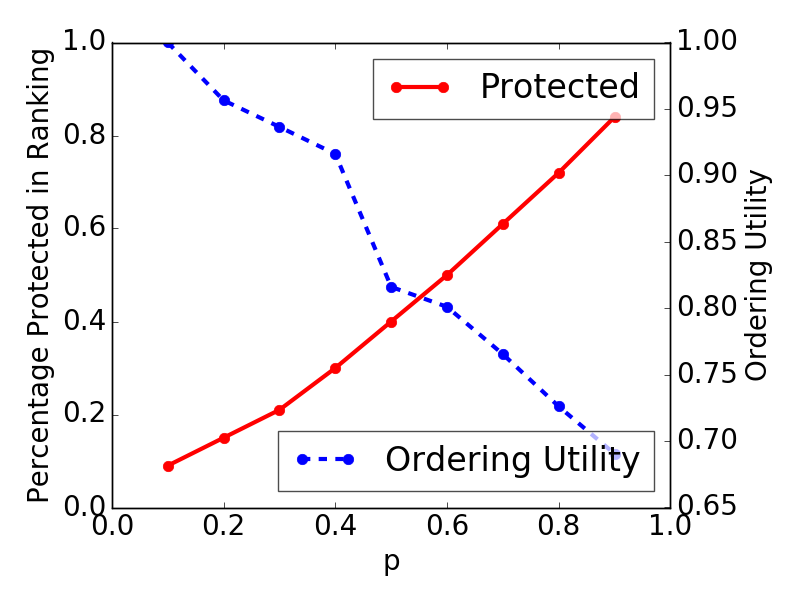
\includegraphics[width=.49\columnwidth]{pics/d4-protected-vs-ordering.png}}
	\subfloat[NDCG]{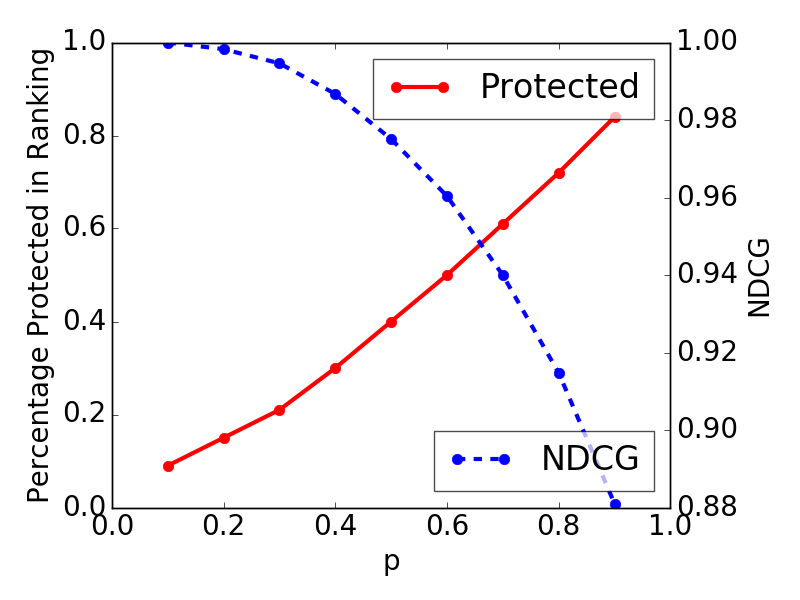
\includegraphics[width=.49\columnwidth]{pics/d4-protected-vs-ndcg.png}}
	\vspace{-2mm}
	\caption{Depiction of possible trade-offs using \algoFAIR. Increase in the percentage of protected candidates in D5 (German credit, protected group age $<$ 25) for increasing values of $p$, compared to %decrease in ordering utility (left) and decrease in NDCG (right).}
		ordering utility and NDCG.}
	\vspace{-\baselineskip}
	\label{fig:results-moving-p}
\end{figure}

%
In this report we describe a correction of the significance adjustment procedure from~\cite{zehlike2017fair}, which did not work for very small $k$ and $\alpha$.
%
For binomial distributions, i.e. where only one protected and one non-protected group is present, the inverse CDF can be stored as a simple table, which we compute using Algorithm~\ref{alg:constructMTable}.
%
We will call such a table \textit{mTable}.
%
\begin{algorithm}[h]
	\caption{Algorithm \algoMtable computes the data structure to efficiently verify or construct a ranking that satisfies binomial ranked group fairness.}
	\label{alg:constructMTable}
	\small
	\AlgInput{$k$, the size of the ranking to produce; $p$, the expected proportion of protected elements; $\alphaadj$, the significance for each individual test.}
	\AlgOutput{$ \mtable $: A list that contains the minimum number of protected candidates required at each position of a ranking of size $k$.}
	$\mtable \leftarrow [k]$ \AlgComment{list of size $k$}
	\For{$i \leftarrow 1$ \KwTo $k$}{
		$\mtable[i] \leftarrow F^{-1}(i,p,\alphaadj)$ \AlgComment{the inverse binomial cdf}
	}
	\Return{$ \mtable $ }
\end{algorithm}

Table~\ref{tbl:ranked_group_fairness_table} shows an example of such a pre-computed table with different $ k $ and $ p $, using $\alpha=0.1$.
%
For instance, for $p=0.5$ we see that at least 1 candidate from the protected group is needed in the top 4 positions, and 2 protected candidates in the top 7 positions.
\begin{table}[h!]
	\small\begin{tabular}{r|cccccccccccc}
		\diaghead{some text}%
		{p}{k}&
		% & \multicolumn{10}{c}{k} \\
		1 & 2 & 3 & 4 & 5 & 6 & 7 & 8 & 9 & 10 & 11 & 12 \\ \midrule
		0.1      & 0 & 0 & 0 & 0 & 0 & 0 & 0 & 0 & 0 & 0  &  0 &  0 \\
		%0.2      & 0 & 0 & 0 & 0 & 0 & 0 & 0 & 0 & 0 & 0  &  1 &  1 \\
		0.3      & 0 & 0 & 0 & 0 & 0 & 0 & 1 & 1 & 1 & 1  &  1 &  2 \\
		%0.4      & 0 & 0 & 0 & 0 & 1 & 1 & 1 & 1 & 2 & 2  &  2 &  3 \\
		0.5      & 0 & 0 & 0 & 1 & 1 & 1 & 2 & 2 & 3 & 3  &  3 &  4 \\
		%0.6      & 0 & 0 & 1 & 1 & 2 & 2 & 3 & 3 & 4 & 4  &  5 &  5 \\
		0.7      & 0 & 1 & 1 & 2 & 2 & 3 & 3 & 4 & 5 & 5  &  6 &  6 \\
		\bottomrule
	\end{tabular}
	\caption{Example values of $m_{\alpha,p}(k)$, the minimum number of candidates in the protected group that must appear in the top $k$ positions to pass the ranked group fairness criteria with $\alpha=0.1$ in a binomial setting.}
	\label{tbl:ranked_group_fairness_table}
\end{table}

Figure~\ref{fig:why-adjustment-is-needed-binomial} shows that we need a correction for $\alpha$ also in the binomial case (note that the scale is logarithmic).
%
In the following, we show that the special case of having only one protected group offers possibilities for verifying ranked group fairness efficiently.
%
A key improvement w.r.t. the more general, multinomial case is that in the binomial setting we can calculate the exact failure probability $\failprob$ (i.e. a fair ranking gets rejected by the ranked group fairness test), which results in an efficient binary search for $\alphaadj$.
%
%Remember that in we had to estimate this probability for mTrees (see Section~\ref{sec:model-adjustment}) using an experimental procedure.

First we introduce the necessary notation for the binomial case and describe how we calculate the exact $\failprob$.
%
Then we show that we can divide the continuum of possible $\alpha$ values in discrete parts in order to be able to apply efficient binary search for the most accurate $\alphaadj$.
%
Last we analyze the complexity of the proposed algorithms.
%This figure is generated by simulation, generating rankings using the process described above and showing the probability of those rankings being rejected by our ranked group fairness test with $\alphaadj=0.1$.
%
%The figure suggests that depending on $k$ we would need to change the value of $\alpha$ if we want to achieve a rejection rate of $0.1$.
\begin{figure}[t!]
	\centering
	{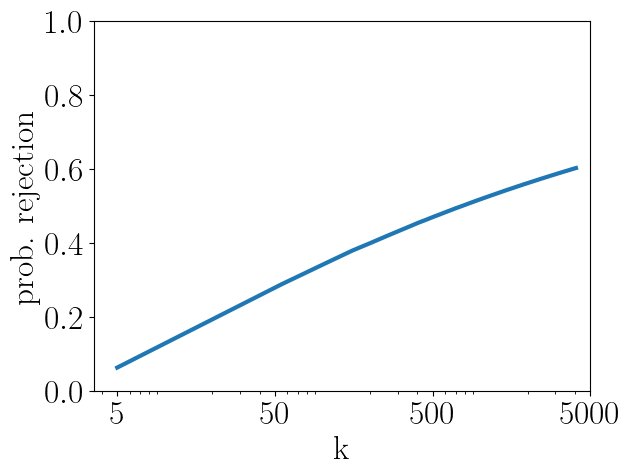
\includegraphics[width=.48\textwidth]{pics/failProbPlotBinom.png}}
	\caption{
		Probability that a fair ranking created by a Bernoulli process with $p=0.5$ fails the ranked group fairness test.\label{fig:why-adjustment-is-needed-binomial}
		%
		Experiments on data generated by a simulation, showing the need for multiple tests correction.
		%
		The data has: one protected group, with a ranking created by  a Bernoulli process (Fig.~\ref{fig:why-adjustment-is-needed-binomial}); and two protected groups, with a ranking created by a multinomial process (Fig.~\ref{fig:why-adjustment-is-needed-multinomial}).
		%
		Rankings should have been rejected as unfair at a rate $\alpha = 0.1$.
		%
		However, we see that the rejection probability increases with $k$.
		%
		Note the scale of $k$ is logarithmic.}
	\label{fig:need-for-model-adjustment}
\end{figure}

\section{Success Probability for One Protected Group}\label{subsubsec:adjustment-binomial}

The probability $\successprob$ that a ranking created following the procedure shown by~\citet{yang2016measuring} passes the ranked group fairness test with parameters $p$ and $\alpha$ can be computed using the following procedure:
%
Let $m(k) = m_{\alpha,p}(k) = F^{-1}(k,p,\alpha)$ be the number of protected elements required up to position $k$.
%
Let $\minv(i) = k$ s.t. $m(k) = i$ be the position at which $i$ or more protected elements are required.
%
Let $b(i) = \minv(i) - \minv(i-1)$ (with $\minv(0) = 0$) be the size of a ``block,'' that is, the gap between one increase and the next in $m(\cdot)$.
%
We call the $k$-dimensional vector $(m(1), m(2), \ldots , m(k))$ a \emph{mTable}.
%
An example is shown on Table~\ref{tbl:05:example_blocks}.
%
\begin{table}[h!]
	\centering
	\begin{tabular}{cccccccccccccc}\toprule
		$k$    & 1 & 2 & 3 & \textbf{{4}} & 5 & 6 & \textbf{7} & 8 & \textbf{9} & 10 & 11 & \textbf{12} \\
		\midrule
		$m(k)$ & 0 & 0 & 0 & \multicolumn{1}{c|}{1} & 1 & 1 & \multicolumn{1}{c|}{2} & 2 & \multicolumn{1}{c|}{3} & 3  & 3  & \multicolumn{1}{c}{4}\\
		Inverse   & \multicolumn{4}{c|}{$\minv(1)=4$}
		& \multicolumn{3}{c|}{$\minv(2)=7$}
		& \multicolumn{2}{c|}{$\minv(3)=9$}
		& \multicolumn{3}{c}{$\minv(4)=12$}\\
		Blocks       & \multicolumn{4}{c|}{$b(1)=4$}
		& \multicolumn{3}{c|}{$b(2)=3$}
		& \multicolumn{2}{c|}{$b(3)=2$}
		& \multicolumn{3}{c}{$b(4)=3$}\\
		\bottomrule
	\end{tabular}
	\caption[Example of different block sizes]{Example of $m(\cdot)$, $\minv(\cdot)$, and $b(\cdot)$ for $p=0.5, \alpha=0.1$.}
	\label{tbl:05:example_blocks}
\end{table}

\noindent Furthermore let
\begin{equation}
	\label{eq:05:combinations}
	I_{m(k)} = \{ v = (i_1, i_2, \ldots, i_{m(k)}): \forall \ell' \in \lbrace 1,\ldots,m(k) -1 \rbrace, 0 \le i_{\ell'} \le b(\ell') \wedge \sum_{j=1}^{\ell'} i_j \ge \ell' \}
\end{equation}
%
represent all possible ways in which a fair ranking\footnote{Note that we do not consider rankings of size 0, which always pass the test.} generated by the method of \citet{yang2016measuring} can pass the ranked group fairness test, with $i_j$ corresponding to the number of protected elements in block $j \; (\text{with } 1 \le j \le k)$.
%
As an example consider again Table~\ref{tbl:05:example_blocks}: the first block contains four positions, i.e. $b(1)=4$ and this block passes the ranked group fairness test, if it contains at least one protected candidate, hence $i_1 \in \{1, 2, 3, 4\}$.
%
The probability of considering a ranking of $k$ elements (i.e. $m(k)$ blocks) unfair, is:
\begin{equation}
	\label{eq:05:failureProb}
	\failprob = 1 - \successprob = 1 - \sum_{v \in I_{m(k)}} \prod_{j=1}^{m(k)} f(v_j; b(j), p)
\end{equation}
%
\noindent where $f(x;b(j),p) = Pr(X = x)$ is the probability density function (PDF) of a binomially distributed variable $X \sim Bin(b(j), p)$.
%
However, if calculated naively this expression is intractable because of the large number of combinations in $I_{m(k)}$.
%

\setlength{\textfloatsep}{2pt}% Remove \textfloatsep
\begin{algorithm}[t!]
	\caption{Algorithm \algoRecursive computes the probability, that a given mTable accepts a fair ranking (see right term of Eq.~\ref{eq:05:failureProb}).}
	\label{alg:05:successProb} % But whenever possible refer to this algo. by name not number
	\small
	\AlgInput{
		$\texttt{b[]}$ list of block lengths (Table~\ref{tbl:05:example_blocks}, 3rd line);\\ 
		$\texttt{maxProtected}$ the sum of all entries of $\texttt{b[]}$;\\
		$\texttt{currentBlockIndex}$ index of the current block; \\
		$\texttt{candidatesAssigned}$ number of protected candidates assigned for the current possible solution; \\
		$p$, the expected proportion of protected elements.}
	\AlgOutput{The probability of accepting a fair ranking.}
	
	\If{$\texttt{b[].length} = 0$}{
		\Return{$1$}
	}
	\tcp{we need to assign at least one protected candidate to each block}
	$\texttt{minNeededThisBlock} \leftarrow \texttt{currentBlockIndex} - \texttt{candidatesAssigned}$\\
	\tcp{if we already assigned enough candidates, minNeededThisBlock = 0 (termination condition for the recursion)}
	\If{$\texttt{minNeededThisBlock} < 0$}{
		$\texttt{minNeededThisBlock} \leftarrow 0$
	}
	$\texttt{maxPossibleThisBlock} \leftarrow \textit{argmin}(\texttt{b[0]}, \texttt{maxProtected})$ \\
	$\texttt{assignments} \leftarrow 0$ \\
	$\texttt{successProb} \leftarrow 0$ \\
	\tcp{sublist without the first entry of $\texttt{b[]}$}
	$\texttt{b\_new[]} \leftarrow \textit{sublist}(\texttt{b[]}, 1, \texttt{b[].length})$ \label{algoline:05:suffixes}\\
	$\texttt{itemsThisBlock} \leftarrow \texttt{minNeededThisBlock}$\\
	\While{$\texttt{itemsThisBlock} \leq \texttt{maxPossibleThisBlock}$}{
		$\texttt{remainingCandidates} \leftarrow \texttt{maxProtected} - \texttt{itemsThisBlock}$ \\
		$\texttt{candidatesAssigned} \leftarrow \texttt{candidatesAssigned} + \texttt{itemsThisBlock}$ \\
		\tcp{each recursion returns the success probability of \emph{all possible ways} to fairly rank protected candidates after this block}
		$\texttt{suffixSuccessProb} \leftarrow \textsc{\algoRecursive} ( $ \\ \pushline $ \texttt{remainingCandidates},\texttt{b\_new[]}, \texttt{currentBlockIndex} + 1,$ \\ $ \texttt{candidatesAssigned})$ 
		\label{algoline:05:recursion}\\
		\popline $\texttt{totalSuccessProb} \leftarrow \texttt{totalSuccessProb} \; + $ \\ \pushline $ \textsc{PDF}(\texttt{maxPossibleThisBlock}, \texttt{itemsThisBlock}, p) \; \cdot $ \\ $ \texttt{suffixSuccessProb}$ \label{algoline:05:pdf}\\
		\popline $\texttt{itemsThisBlock} \leftarrow \texttt{itemsThisBlock} + 1$\\
	}
	\Return{probability of accepting a fair ranking: $\texttt{totalSuccessProb}$ }
\end{algorithm}
We therefore propose a dynamic programming method, Algorithm~\ref{alg:05:successProb}, which computes the probability that a fair ranking passes the ranked group fairness test (i.e. the right term of Equation~\ref{eq:05:failureProb}) \emph{recursively}.
%
Note that because of the combinatorial complexity of the problem a \emph{simple closed-form expression} to compute $\failprob$ is unlikely to exist.
%With this algorithm however, we have to account for an important pitfall: we may choose a combination of $k, p, \alpha$ where the last block ``reaches beyond'' $k$.
%
%Consider again Table~\ref{tbl:05:example_blocks} with $k=8, \minpro$p=$0.5, \alpha=0.1$: the second block reaches until position 7, while the third block reaches until position 9.
%
%If we cut off the mTable at $k=8$ to adjust the significance level, the last block reaches beyond $k$ which is to position 9.
%
%\meike{Inwiefern macht der neue Algorithmus das Problem mit aufgebrochenen Blöcken besser?}
%To account for that t
The algorithm breaks the vector $v = (i_1, i_2, \ldots ,i_{\ell})$ of Equation~\ref{eq:05:combinations} into a \textit{prefix} and a \textit{suffix} (Alg.~\ref{alg:05:successProb}, Line~\ref{algoline:05:suffixes}).
%
We call $i_1$ the \textit{prefix} of $(i_2, \ldots, i_{\ell})$, and $(i_2, \ldots, i_{\ell})$ the \textit{suffix} of $i_1$.
%
The algorithm starts with a prefix and calculates all possible suffixes, that pass the ranked group fairness test, recursively (Line~\ref{algoline:05:recursion}).
%
Consider the following example: for the first prefix $i_1 = 1$ the algorithm computes all possible suffixes, where we rank exactly one protected candidate in the first block.
%
For this prefix $i_1$, combined with each possible suffix $v \setminus i_1$, we calculate the success probability $\prod_{j=1}^{m(k)} f(v_j; b(j), p)$ for each instance of $v$ (Line~\ref{algoline:05:pdf}).
%
In the next recursion level we start with a new prefix, let us say $i_1=1, i_2 =1$.
%
The algorithm computes all possible suffixes, i.e. all rankings where we rank exactly one protected candidates in the first block and one protected candidate in the second block.
%
Then it computes the respective success probabilities.
%
This procedure continues for $m(k)$ iterations.
%
After that the whole program starts again with $i_1=2$ and is repeated until the maximum number of protected candidates is reached, in our case $b(1)=4$.
%
All intermediate success probabilities are added up (Line~\ref{algoline:05:pdf}) to the total success probability (see Eq.~\ref{eq:05:failureProb}) of the mTable that was created given $k, p, \alpha$.

Note that there are at most $\prod_{j=1}^{m(k)}b(j)$ possible combinations to distribute the protected candidates within the blocks.
%
Furthermore many $v \in I_{m(k)}$ share the same prefix and hence have the same probability density value for these prefixes.
%
To reduce computation time the algorithm stores the binomial probability density value for each prefix in a hash map with the prefix as key and the respective pdf as value.
%
Thus the overall computational complexity becomes $O(\prod_{j=1}^{m(k)}b(j) \cdot O(\texttt{binomPDF}))$.

\section{Finding the Correct mTable}\label{subsec:finding-mtable}
We call an mTable \textit{correct} if it has an overall success probability of $\successprob = 1-\alpha$.
However, given parameters $k,p,\alpha$, $\successprob$ will be greater or equal to $1-\alpha$. Thus, we need a corrected $\alphaadj \leq \alpha$ in order to compute the correct mTable. Unfortunately there is no way to compute $\alphaadj$ directly, which is why we have to search for the correct mTable, hence $\alphaadj$.
We propose Algorithm~\ref{alg:05:binarySearch} that takes  parameters $k, p, \alphaadj$ as input and returns the correct mTable and $\alphaadj$.
%
%We use Algorithm~\ref{alg:05:successProb} to determine the adjusted significance level $\alphaadj$ for the ranked group fairness test, such that the overall acceptance probability for the mTable with parameters $k, p, \alphaadj$ becomes $1-\alpha$.
%
It sequentially creates mTables (recall that these are $k$-dimensional vectors of the form $(m(1), m(2), \ldots , m(k))$) for different values of $\alphaadj$, and then calls Algorithm~\ref{alg:05:successProb} to calculate their success probability until it finds the correct mTable with overall failure probability $\failprob = \alpha$ .
%
Our goal is to use binary search to select possible candidates for $\alphaadj$ systematically.

%\note[ChaTo]{Perhaps the definition of the mass of an mTable can wait a few more paragraphs, until you need it.}
However, to be able to do binary search, we need a discrete measure for the $\alpha$-space to search on, otherwise the search would never stop. Specifically, we could never be sure if we found the mTable with the minimum difference of $\successprob$ to $1-\alpha$. A binary search would further and further divide an interval between two $\alpha$ values. The only chance to verify that we do not have to search further is by comparing the resulting mTables of different $\alpha$ values. We will see, that we can do that by comparing the sum of the entries in the mTable and that there exist only a limited number of them.
%
Furthermore, to reduce complexity we only want to consider mTables with certain properties, which we define in the following paragraph.
%
A $k$-dimensional vector (e.g. $(0,0,1,2,3)$) has to have two properties in order to constitute a mTable, rather than just a vector of natural numbers: it has to be \emph{valid} and \emph{legal}.
%
\begin{definition}[Valid mTable]
	\label{def:05:valid-mtable}
	The $\text{mTable}_{p,k,\alpha}=(m(1) , m(2) , \ldots , m(k))$ is \emph{valid} if and only if, $m(i) \leq m(j)$ for all $i,j \in \lbrace 0, \ldots, k \rbrace$ with $i < j$ and $m(i)=n \Rightarrow m(i+1) \leq n+1$.
\end{definition}
\noindent It is easy to see that many valid mTables exist.
%
They correspond to all $k$-dimensional arrays with integers monotonically increasing by array indices.
%
However we only want to consider those valid mTables for our ranked group fairness test that have been created by the statistical process in~\citet{yang2016measuring}.
%
We call these \textit{legal mTables}.
%
\begin{definition}[Legal mTable]
	\label{def:05:legal-mtable}
	A $\text{mTable}_{p,\alpha,k}$ is \textit{legal} if and only if there exists a $p,k,\alpha$ such that
	$\texttt{constructMTable}(p,k,\alpha)=\text{mTable}_{p,\alpha,k}$.
\end{definition}
%
Definition \ref{def:05:legal-mtable} restricts the space of k-dimensional arrays to those which are computed by a specific function. Since the mTable is a datastructure that should represent the minimum proportions required for a specific dice roll, we have to define $\texttt{constructMTable}$ such that it represents this process. Otherwise we could think of various ways to define processes to compute possible mTables.
\begin{definition}[constructMTable]
	\label{def:05:construct-mtable-single-test}
	For $p\in [0,1], k \in \mathbb{N}, \alpha \in [0,1]$ we define a function to construct a mTable from input parameters $p, k, \alpha$ according to \cite{yang2016measuring}.

	\noindent$\texttt{constructMTable} : \\ (0,1) \times \mathbb{N} \times [0,1] \longrightarrow \lbrace (m(1) ,\ldots, m(k)): m(i) = F^{-1}(i,p,\alpha), \, i = \{1,\ldots,k\}\rbrace$ \\
	with $\texttt{constructMTable}(p,k,\alpha)=\text{mTable}_{p,k,\alpha}$.
\end{definition}
%
\begin{lemma}
	\label{lemma:05:legal-valid-mtable}
	If a mTable is legal, it is also valid.
\end{lemma}
%
\noindent Lemma \ref{lemma:05:legal-valid-mtable} follows directly by construction.
%
Now we need a discrete partition of the continuous $\alpha$ space, that is a discrete measure that corresponds to exactly one legal mTable for a given set of parameters $k,p,\alpha$.
%
We call this measure the \emph{mass} of a mTable.
%The definition of a legal mTable together with its corresponding mass enables us to perform a binary search, which helps us to find $\alphaadj$ and hence the correct mTable with an overall failure probability of $\alpha$.
%
%Note that for any value of $\alpha$ there exists exactly one \emph{legal} mTable.
%
%However, the opposite is not true: as $\alpha$ is a real number from the interval $[0, 1]$, the same mTable can be created using different (but very similar) values of $\alpha$.
%
%Thus without a discrete measure for a mTable we do not know when to stop searching, which is why we introduce the \emph{mass of a mTable}.
%
\begin{definition}[Mass of a mTable]
	\label{def:05:Mass of a MTable}
	For $\text{mTable}_{p,k,\alpha}=(m(1) , m(2) , \ldots , m(k))$ we call\\
	$L_1(\text{mTable}_{p,k,\alpha})=\sum_{i=1}^k m(i)$ the \textit{mass of $\text{mTable}_{p,\alpha,k}$}.
\end{definition}
%
In the following we relate the continuous $\alpha$-space to the discrete mass of a mTable.
%
\begin{lemma}
	\label{lemma:05:non-decreasing-with-alpha-mtable}
	Every $\text{mTable}_{p,k,\alpha}=\texttt{constructMTable}(p,k,\alpha)=(m(1) , m(2) , \ldots , m(k))$ is non-decreasing with $\alpha$. This means that
	$\texttt{constructMTable}(p,k,\alpha - \epsilon) = (m(1)' , m(2)' , \ldots , m(k)')$ will result in $m(i)' \leq m(i)$ for $i=1,\ldots,k$ and $\epsilon > 0$.
\end{lemma}
\begin{proof}
\label{proof:05:non-decreasing-with-alpha-mtable}
Every entry $m(i)$ for $i=1,\ldots,k$ is computed by line 3 of Algorithm~\ref{alg:constructMTable}, i.e. every entry is the inverse binomial cdf $F^{-1}(i,p,\alphaadj)$. In other words $m(i)$ is the smallest integer such that\\
\begin{equation}
\alphaadj \leq \sum_{j=0}^{m(i)}\binom{i}{j}p^i (1-p)^{i-j} = F^{-1}(i,p,\alphaadj)
\end{equation}
The following equivalence holds:
\begin{equation}\label{eq:smaller m}
\alphaadj - \epsilon \leq \sum_{j=0}^{m'(i)}\binom{i}{j}p^i (1-p)^{i-j} = F^{-1}(i,p,\alphaadj-\epsilon)
	\Leftrightarrow \alphaadj \leq \sum_{j=0}^{m'(i)}\binom{i}{j}p^i (1-p)^{i-j} + \epsilon
\end{equation}
Now suppose that $m'(i) > m(i)$ which contradicts lemma \ref{lemma:05:non-decreasing-with-alpha-mtable}.
%
Then it is that
\[m'(i)>m(i) \Rightarrow \sum_{j=0}^{m'(i)}\binom{i}{j}p^i (1-p)^{i-j} \geq \sum_{j=0}^{m(i)}\binom{i}{j}p^i (1-p)^{i-j}\]
because $\binom{i}{j}p^i (1-p)^{i-j} \geq 0 \; \forall i,j,p$. It follows for $\epsilon >0$ that
\begin{equation}
\alphaadj \leq \sum_{j=0}^{m(i)}\binom{i}{j}p^i (1-p)^{i-j} + \epsilon \leq \sum_{j=0}^{m'(i)}\binom{i}{j}p^i (1-p)^{i-j} + \epsilon
\end{equation}
But then $m'(i)\neq F^{-1}(i,p,\alphaadj-\epsilon)$ because $m(i)$ would be the smaller integer that satisfies Equation~\ref{eq:smaller m}. Thus it has to be that $m'(i)\leq m(i)$.
\end{proof}
%
\noindent This property shows that, if we reduce $\alpha$ in our binary search, the mass of the corresponding mTable is also reduced or stays the same.
%
It very usefully implies a criterion to stop the binary search: namely we stop the calculation when the mass of the mTable at the left search boundary equals the right search boundary.
%
Of course this only works if there exists exactly one legal mTable for each mass, which we proof in the following.
\begin{theorem}
	\label{theorem:05:mtable-mass-injection}
	For fix $p,k$ there exists exactly one legal mTable for each mass $L_1\in \lbrace 1,\ldots,k \rbrace$.
\end{theorem}
%
\begin{proof}
	\label{proof:05:mtable-mass-injection}
	We prove this by contradiction: Let $MT_{p,k,\alpha_1}$ and $MT'_{p,k, \alpha_2}$ be two different mTables with $L_1(MT_{p,k,\alpha_1 }) = L_1(MT'_{p,k,\alpha_2})$.\\
	%
	If both are legal then it applies that $\texttt{constructMTable}(p,\alpha_1 ,k)=MT_{p,\alpha_1 ,k}$
	and \\ $\texttt{constructMTable}(p,\alpha_2 ,k)=MT'_{p,\alpha_2 ,k}$.
	%
	Because $MT_{p,k,\alpha_1} \neq MT'_{p,k,\alpha_2}$, without loss of generality entries $m(i), m(i)' , m(j) , m(j)'$ exist in each table, such that $|m(i) - m(i)'| = |m(j) - m(j)'|$ while at the same time $m(i) > m(i)'$ , $m(j) < m(j)'$ for $i<j, i,j \in \lbrace 1, \ldots , k \rbrace$.
	%
	(Think of it as the two entries in each table "evening out", such that both tables have the same mass.)\\
	%
	If $\alpha_1 > \alpha_2$, then the statement $m(j)' > m(j)$ violates Lemma~\ref{lemma:05:non-decreasing-with-alpha-mtable}.
	%
	If $\alpha_2 > \alpha_1$, then the statement $m(i) > m(i)'$ also violates Lemma~\ref{lemma:05:non-decreasing-with-alpha-mtable}.
	%
	The only possibility left is hence that $\alpha_1 = \alpha_2$, which contradicts $MT \neq MT'$, as both are created using function \texttt{constructMTable}.
\end{proof}
%
With these mathematical properties we can perform a binary search on the continuous $\alpha$-space to find the corrected significance level $\alphaadj$.
%
This corrected significance is used to compute a final mTable with an overall failure probability $\failprob = \alpha$.
\begin{algorithm}[t!]
	\caption{Algorithm \algoBinomBinary calculates the corrected significance level $\alpha_c$ and the mTable $m_{\alpha_c , k, p)}$ with an overall probability $\alpha$ of rejecting a fair ranking.}
	\label{alg:05:binarySearch} % But whenever possible refer to this algo. by name not number
	\footnotesize
	\AlgInput{$k$, the size of the ranking to produce; $p$, the expected proportion of protected elements; $\alpha$, the desired significance level.}
	\AlgOutput{$\alphaadj$ the adjusted significance level; \texttt{m\_{adjusted}} the adjusted mTable}
	\AlgComment{initialize all needed variables}
	\texttt{aMin $\leftarrow$ 0};
	\texttt{aMax $\leftarrow \alpha$ };
	\texttt{aMid} $\leftarrow \frac{(\texttt{aMin + aMax})}{2}$ \\
	\texttt{m\_min} $\leftarrow$ \texttt{constructMTable(k,p,aMin)}; 
	\texttt{m\_max} $\leftarrow$ \texttt{constructMTable(k,p,aMax)}; \\
	\texttt{m\_mid} $\leftarrow$ \texttt{constructMTable(k,p,aMid)} \\
	\texttt{maxMass} $\leftarrow$ \texttt{m\_max.getMass()};
	\texttt{minMass} $\leftarrow$ \texttt{m\_min.getMass()};
	\texttt{midMass} $\leftarrow$ \texttt{m\_mid.getMass()}\\
	
	\While{\texttt{minMass} $<$ \texttt{maxMass} AND \texttt{m\_mid.getFailProb()} $\neq \alpha$ }{
		\If{\texttt{m\_mid.getFailProb()} $< \alpha$}{
			\texttt{aMin} $\leftarrow$ \texttt{aMid}
			\texttt{m\_min} $\leftarrow$ \texttt{constructMTable(k,p,aMin)} \\
		}
		\If{\texttt{m\_mid.getFailProb()} $> \alpha$}{
			\texttt{aMax} $\leftarrow$ \texttt{aMid} \\
			\texttt{m\_max} $\leftarrow$ \texttt{constructMTable(k,p,aMax)} \\
		}
		\texttt{aMid} $\leftarrow \frac{(\texttt{aMin + aMax})}{2}$ \\
		\tcp{stop criteria if midMass equals maxMass or midMass equals minMass}
		\If{\texttt{maxMass - minMass == 1}}{
			\texttt{minDiff} $\leftarrow |$\texttt{m\_min.getFailProb() - }$\alpha|$ \\
			\texttt{maxDiff} $\leftarrow |$\texttt{m\_max.getFailProb() - }$\alpha|$ \\
			\tcp{return the $\alpha_c$ which has the lowest difference from the desired significance}			
			\If{\texttt{minDiff} $<$ \texttt{maxDiff}}{
				\Return{\texttt{aMin, m\_min}}
			}
			\Else{
				\Return{\texttt{aMax, m\_max}}
			}
		}
		\tcp{stop criteria if midMaxx is exactly the mass between minMass and maxMass}
		\If{\texttt{maxMass - midMass == 1} AND \texttt{midMass - minMass == 1}}{
			\texttt{minDiff} $\leftarrow |$\texttt{m\_min.getFailProb() - }$\alpha|$ \\
			\texttt{maxDiff} $\leftarrow |$\texttt{m\_max.getFailProb() - }$\alpha|$ \\
			\texttt{midDiff} $\leftarrow |$\texttt{m\_mid.getFailProb() - }$\alpha|$ \\
			\tcp{return the $\alpha_c$ which has the lowest difference from the desired significance}			
			\If{\texttt{midDiff} $\leq$ \texttt{maxDiff} AND \texttt{midDiff} $\leq$ \texttt{minDiff}}{
				\Return{\texttt{aMid, m\_mid}}
			}
			\If{\texttt{minDiff} $\leq$ \texttt{midDiff} AND \texttt{minDiff} $\leq$ \texttt{maxDiff}}{
				\Return{\texttt{aMin, m\_min}}
			}
			\Else{
				\Return{\texttt{aMax, m\_max}}
			}
		}
	}
	\Return{\texttt{aMid, m\_mid}}
\end{algorithm}

\section{Complexity Analysis}

In order to estimate the complexity of the whole procedure (and hence understand its computational feasibility), we need to know how many mTables exist for fix $k$ and $p$.
%
%\note[ChaTo]{@Tom: please check if the following sentence that I added is correct, I thought it would make this more understandable.}
This is the number of non-decreasing sequences of integers that end with a number smaller or equal to $k$ and have length~ $k$.
%
\begin{theorem}
	\label{theorem:05:number-of-mtables}
	The number of legal mTables for $k,p$ is less or equal to $\frac{k(k-1)}{2}$ .
\end{theorem}

\begin{proof}
	\label{proof:05:number-of-mtables}
	Given the proof of Theorem~\ref{theorem:05:mtable-mass-injection} we can count the number of legal mTables for fix $p,k$ as follows: The maximum mass of a legal mTable of length $k$ is by construction
	$L_1 ((m(1) = 1,m(2) = 2, \ldots, m(k) = k)) = \sum_{i=1}^k m(i) = \frac{k(k-1)}{2}$.
	%
	Following definition~\ref{def:05:valid-mtable} the 	    entry $m(1)$ is the smallest entry or equal to all other entries.
	%
	Furthermore, because this mTable is legal and following Definition~\ref{def:05:legal-mtable}, the mTable is a result of Algorithm~\ref{alg:constructMTable}.
	%
	Thus $m(1) = F^{-1}(1,p,\alpha) \in \lbrace 0,1\rbrace$. In other words, $m(1)$ can only be $0$ or $1$.

	%
	In turn $m(2)$ can only be $2$, if $m(1)$ was $1$ (otherwise $m(2)<2$).
	%
	Accordingly, the minimum mass of a legal mTable is $L_1((m(1),m(2), \ldots, m(k))) = 0$, if all $m(i)=0$.
	%
	Following Lemma~\ref{lemma:05:non-decreasing-with-alpha-mtable}, we can create mTables with higher masses by increasing $\alpha$.
	%
	Furthermore, following Theorem~\ref{theorem:05:mtable-mass-injection}, if a legal mTable exists for a given mass and parameters $k,p$, then this is the only existing legal mTable with that mass.
	%
	We know that there is a theoretical minimum mass for legal mTables ($L_1 =0$) which would occur, for example, if we set $\alpha = 0$ assuming $p<1$.
	%
	There also exists a theoretical maximum mass for legal mTables which is $\frac{k(k-1)}{2}$.
	%
	At best, we can achieve every possible mass between those two to extremes.
	%
	It follows that there are at most $\frac{k(k-1)}{2}$ masses for legal mTables of size $k$ for a fix~$p$.
\end{proof}
%
\subsubsection{\algoMtable complexity}\label{subsubsec:construct-mtable-complexity}
\algoMtable computes the inverse binomial cdf for $k$ positions of the ranking and stores each of the computed values in the MCDF Cache.
%
This leads to a time complexity of $\mathcal{O}(k) \cdot \mathcal{O}(F^{-1}(p,k,\alpha))$.
%
Assuming a constant time for the calculation of the binomial probability mass function, the time complexity of $F^{-1}(p,k,\alpha)$ for our implementation is $\mathcal{O}(i^2)$, where $i$ is the current position we calculate $F^{-1}$ for.
%
Note that the complexity of $F^{-1}$ depends on the desired accuracy of the computation.
%
The space complexity is $\mathcal{O}(k)$, if we do not store any intermediate results for future calculations.
%
\begin{table}[b!]
	\scalebox{0.75}{
		\begin{tabular}{lll}
			\toprule
			\textbf{Algorithm} & \textbf{Time Complexity} & \textbf{Space Complexity}\\
			\midrule
			\rowcolor[HTML]{C0C0C0}
			\algoMtable & $\mathcal{O}(k) \cdot \mathcal{O}(F^{-1}(p,k,\alpha))$ & $\mathcal{O}(k)$ \\
			\algoRecursive & $\mathcal{O}(\texttt{\algoMtable}) + \mathcal{O}(\prod_{j=1}^{m(k)}b(j) \cdot O(\texttt{binomPDF}))$ & $\mathcal{O}(k)$ \\
			\rowcolor[HTML]{C0C0C0}
			\algoBinomBinary & $\mathcal{O}(\log{}k) \cdot (\mathcal{O}(\texttt{\algoRecursive}))$ & $\mathcal{O}(k)$  \\
			\bottomrule
		\end{tabular}
	}
	\caption{Time complexity for all algorithms for one protected group without pre-computed results.\label{tbl:time-space-binom}}
\end{table}

\subsubsection{\algoRecursive complexity}\label{subsubsec:success-prob-complexity}
The algorithm \algoRecursive has time complexity $\mathcal{O}(\prod_{j=1}^{m(k)}b(j) \cdot O(\texttt{binomPDF}))$ as explained in section \ref{subsubsec:adjustment-binomial}.
%
Before we compute the success probability, we have to calculate the corresponding mTable and blocks $b$ which adds $\mathcal{O}(k) \cdot \mathcal{O}(F^{-1}(p,k,\alpha))$ and $\mathcal{O}(k)$ to the time complexity of \algoRecursive.
%
Overall we get $\mathcal{O}(k) \cdot \mathcal{O}(F^{-1}(p,k,\alpha)) + \mathcal{O}(\prod_{j=1}^{m(k)}b(j) \cdot O(\texttt{binomPDF}))$.
%
For the sake of readability we will write $\mathcal{O}($\algoMtable$) + \mathcal{O}(\prod_{j=1}^{m(k)}b(j) \cdot O(\texttt{binomPDF}))$.
%
The space complexity is $\mathcal{O}(k)$ for the maximum number of blocks plus $\mathcal{O}(k)$ for the stored probabilities at each position.
%
\subsubsection{\algoBinomBinary complexity}\label{subsubsec:binom-binary-complexity}
A general binary search on a list of $n$ items has a time complexity of $\mathcal{O}(\log{}n)$. We showed with theorem \ref{theorem:05:number-of-mtables} that the list of mTables on which we will search binary, has a maximum size of $\frac{k(k-1)}{2}$.
Thus the binary search for $\alpha_c$ has a complexity of $\mathcal{O}(\log{}\frac{k(k-1)}{2}) = \mathcal{O}(\log{}k^2) = \mathcal{O}(\log{}k)$.
%
For each binary search step we need $\mathcal{O}(\mathcal{O}(k) \cdot \mathcal{O}(F^{-1}(p,k,\alpha)))$ to compute the new mTable, as well as $\mathcal{O}(\prod_{j=1}^{m(k)}b(j) \cdot O(\texttt{binomPDF}))$ for its fail probability.
%
Overall we get $\mathcal{O}(\log{}k) \cdot (\mathcal{O}(\prod_{j=1}^{m(k)}b(j) \cdot O(\texttt{binomPDF})) + \mathcal{O}(\mathcal{O}(k) \cdot \mathcal{O}(F^{-1}(p,k,\alpha))))$, which we will write as $\mathcal{O}(\log{}k) \cdot (\mathcal{O}(\texttt{\algoRecursive}))$.
%
The space complexity is $\mathcal{O}(k)$ since we only store the three mTables with their respective fail probability at a time.


%!TeX root=main.tex
\section{Conclusions}\label{sec:conclusions}

In this paper we presented the extension of \algoFAIR to multiple groups, where we guarantee ranked group fairness, without introducing a large utility loss.
%
Especially when groups largely have the same utility score in the top positions (as is the case in the COMPAS experiments) no ranking utility at all is lost in terms of NDCG or individual fairness.
%
In this case \algoFAIR only benefits the protected groups without skewing the ranking result.
%
If a protected group already receives advantageous exposure in the colorblind ranking and the ranked group fairness condition is already met via the ranking scores of the candidates, \algoFAIR preserves this.
%
A protected candidate can only lose exposure due to a protected candidate from another group being ranked up, but not due to a non-protected one.
%
Additionally the user can control the degree of fairness that is obtained in the result by setting $p_G$ to a value that is appropriate for the situation at hand.
%
This lets them transparently control the trade-off between fairness and utility, instead of having a less intuitive fairness parameter $\theta$ that operates on the barycenter of group distributions.

\spara{Future work.}
%
An important challenge is the algorithmic complexity of calculating the mTree for a particular configuration of $p_G$ and $\alpha$.
%
Though we already implemented improvements to reduce complexity, calculating an adjusted mTree of length $k=100$ with six groups takes several weeks.
%
Of course this mTree has to be calculated only once and can then be persistent and shared among users of \algoFAIR, however when a situation demands a new configuration these calculation times are currently unavoidable.
%
A significant speed-up could be achieved by programming a customized mcdf-function which can store the results of repetitive computation steps.
%
This is however very memory-intensive and the algorithm then needs to run on large computer clusters.
%
Additionally one could provide a script that fills the MCDF Cache with various configurations of $p_G$ and $\alpha$.
%
This calculation can continuously run as a separate process on a server which then provides the obtained caches to users who want to compute new mTrees.

One of the main challenges for fair ranking algorithms in general is that there is not yet much empirical evidence that re-ordering items actually helps to overcome the bias in click-probability across groups.
%
Recent research \cite{suhr2020does}, however,  suggests that guarantees for a minimum representation of underrepresented groups yield to higher selection rates in different hiring contexts, but does not mitigate user biases completely. For example if a user prefers male candidates for a moving assistance task over female candidates, ranking female candidates higher will not mitigate users' biases completely.
%
Thus, a method such as \algoFAIR may be able to increase the click probability for protected groups. Furthermore, setting the values for $p_G$ higher than desired may mitigate user biases. For example, it might be effective to set the minimum proportion for the protected group women in the context of hiring for moving assistance to $60\%$ in order to achieve a click probability of $50\%$ for this group.
%
However further research has to be conducted to study the effect on users of re-ordering items in a ranking and to understand the best means to overcome these strong prejudices against minority groups in certain domains.
%
\changed{This is an empirical question that needs to be addressed through user studies; approaches based on simulating clicks using pre-existing user preferences, such as the one used by \citet{abdollahpouri2021user}, may not uncover the actual interplay between the displayed ranking and latent user preferences.}
%
Additionally, further experimental research using synthetic data could allow us to test with a wider range of differences across groups, larger than the one that real datasets exhibit.
%
Finally, robustness tests to measure the sensitivity of the rankings to noise in the qualification/score inputs could be helpful to determine to what extent they may affect our fairness objectives.

\spara{Reproducibility.}
Code and data that can be used to reproduce the experiments on this paper is available: \url{https://github.com/MilkaLichtblau/Multinomial_FA-IR}.

\section{Acknowledgements}

This research was supported by the Max Planck Institute for Software Systems, the German Research Foundation and the Catalonia Trade
and Investment Agency (ACCI{\'O}).
%
M.Z. was supported by the MPI and the GRF.
%
C.C. was partially supported by "la Caixa" Foundation (ID 100010434), under the agreement LCF/PR/PR16/51110009.
%
%T.S. was supported by his parents.


%%%%%%%%%%%%%%%%%%%%%%%%%%%%%%%%%%%%%%%%%%%%%%%%%%%%%%%%%%%%%%%%%%
% BIBLIOGRAPHY
%%%%%%%%%%%%%%%%%%%%%%%%%%%%%%%%%%%%%%%%%%%%%%%%%%%%%%%%%%%%%%%%%%

% This must be close to the FIRST column of the last page
% Otherwise it's too late to balance
%\balance

% Bibliography style and items
\bibliographystyle{ACM-Reference-Format}
\bibliography{main}
\appendix
%!TEX root = main.tex
\section{Appendix}
\label{sec:appendix}
\begin{table}[h!]
	\caption{Adjusted significance $\alphaadj$ obtained by using \algoCorrect with $\alpha=0.1$ for selected $k, p$. For small values of $k, p$ there is no $\alphaadj$ that yields the required significance.}
	\vspace{-3mm}
	\label{tbl:alpha_corrected}
	\small\begin{tabular}{r|cccc}
		\diaghead{soi text}%
		{$\;$\\p}{k}&
		%    & \multicolumn{4}{c}{$k$} \\
		$40$ & $100$ & $1,000$ & $1,500$ \\\midrule
		0.1 & -- & -- & 0.0140 & 0.0122 \\
		0.2 & -- & -- & 0.0115 & 0.0101 \\
		0.3 & -- & 0.0220 & 0.0103 & 0.0092 \\
		0.4 & -- & 0.0222 & 0.0099 & 0.0088 \\
		0.5 & 0.0168 & 0.0207 & 0.0096 & 0.0084 \\
		0.6 & 0.0321 & 0.0209 & 0.0093 & 0.0085 \\
		0.7 & 0.0293 & 0.0216 & 0.0094 & 0.0084 \\
		\bottomrule
	\end{tabular}
\end{table}

\begin{algorithm}[h]
	\caption{Algorithm \algoCorrect used to compute model adjustment. Note that for notational convenience, vector indexes start at zero. Operator ``$>>$'' shifts vector components to the right, padding on the left with zeros.}
	\label{alg:correction} % But whenever possible refer to this algo. by name not number
	\small
	\AlgInput{$k$, the size of the ranking to produce; $p$, the expected proportion of protected elements; $\alphaadj$, the significance for each individual test.}
	\AlgOutput{The probability of rejecting a fair ranking.}
	$(m_{\operatorname{old}},i_{\operatorname{old}}) \leftarrow (0, 0)$ \AlgComment{Auxiliary vectors}
	\For{$i \leftarrow 1$ \KwTo $k$}{
		$m[i] \leftarrow F^{-1}(\alphaadj; i, p)$ \\
		\If{$m[i] > m_{\operatorname{old}}$}{
			$\minv[m_{\operatorname{old}}] \leftarrow i$ \\
			$b[m_{\operatorname{old}}] \leftarrow i - i_{\operatorname{old}}$ \\
			$(m_{\operatorname{old}},i_{\operatorname{old}}) \leftarrow (m[i], i)$ \\
		}
	}
	$S[0] \leftarrow 1$ \AlgComment{Success probabilities}
	\For{$j \leftarrow 1$ \KwTo $m(k)$}{
		$S_{\operatorname{new}} \leftarrow$ zero vector of dimension $j$ \\
		\For{$i \leftarrow 0$ \KwTo $b(j)$}{
			\AlgComment{$f(i;b(j),p)$ is the prob. mass of $Bin(b(j),p)$}
			$S_{\operatorname{new}} \leftarrow S_{\operatorname{new}} + ( S >> i ) \cdot f(i; b(j), p)$ \\
		}
		$S_{\operatorname{new}}[j-1] \leftarrow 0$ \\
		$S \leftarrow S_{\operatorname{new}}$ \\
	}
	\Return{probability of rejecting a fair ranking: $1 - \sum S[i]$ }
\end{algorithm}

\begin{algorithm}[h!]
	\caption{Algorithm \algoMultBinary calculates the corrected significance level $\alpha_c$ such that the mTree $m(\alpha_c , k, p_G)$ has the probability of rejecting a fair ranking $\alpha$}
	\label{alg:mult_binary} % But whenever possible refer to this algo. by name not number
	\small
	\AlgInput{$k$, the size of the ranking to produce; $p_G$, the vector of expected proportions of protected elements; $\alpha$, the desired significance level, $\epsilon$ the tolerance for variance in the experimental fail probability calculation.}
	\AlgOutput{$\alphaadj$ the adjusted significance level, \texttt{m\_{adjusted}} the adjusted mTree}
	\AlgComment{initialize all needed variables}
	\texttt{aMin $\leftarrow$ 0};
	\texttt{aMax $\leftarrow \alpha$ };
	\texttt{aMid} $\leftarrow \frac{(\texttt{aMin + aMax})}{2}$ \\
	\texttt{m\_min} $\leftarrow$ \texttt{computeMTree(k,$p_G$,aMin)} 
	\texttt{m\_max} $\leftarrow$ \texttt{computeMTree(k,$p_G$,aMax)}
	\texttt{m\_mid} $\leftarrow$ \texttt{computeMTree(k,$p_G$,aMid)} \\
	
	\While{True}{
		\If{\texttt{m\_mid.getFailProb()} $< \alpha$}{
			\texttt{aMin} $\leftarrow$ \texttt{aMid} \\
			\texttt{m\_min} $\leftarrow$ \texttt{computeMTree(k,$p_G$,aMin)} \\
			\texttt{aMid} $\leftarrow$ $\frac{\texttt{aMin}+\texttt{aMax}}{2}$ \\
			\texttt{m\_mid} $\leftarrow$ \texttt{computeMTree(k,$p_G$,aMid)}
		}
		\If{\texttt{m\_mid.getFailProb()} $> \alpha$}{
			\texttt{aMax} $\leftarrow$ \texttt{aMid} \\
			\texttt{m\_max} $\leftarrow$ \texttt{computeMTree(k,$p_G$,aMax)} \\
			\texttt{aMid} $\leftarrow$ $\frac{\texttt{aMin}+\texttt{aMax}}{2}$ \\
			\texttt{m\_mid} $\leftarrow$ \texttt{computeMTree(k,$p_G$,aMid)}
		}
		\tcp{compute all differences between fail probability and $\alpha$}
		\texttt{midDiff} $\leftarrow$ $|\texttt{m\_mid.getFailProb()} - \alpha|$ \\
		\texttt{maxDiff} $\leftarrow$ $|\texttt{m\_max.getFailProb()} - \alpha|$ \\
		\texttt{minDiff} $\leftarrow$ $|\texttt{m\_min.getFailProb()} - \alpha|$ \\
		\tcp{case where midDiff is the the smallest difference from desired significance}
		\If{\texttt{midDiff} $\leq \epsilon$ AND \texttt{midDiff} $\leq \texttt{maxDiff}$ AND \texttt{midDiff} $\leq \texttt{minDiff}$}{
			\Return{\texttt{aMid, m\_mid}}
		}
		\tcp{case where minDiff is the the smallest difference from desired significance}
		\If{\texttt{minDiff} $\leq \epsilon$ AND \texttt{minDiff} $\leq \texttt{maxDiff}$ AND \texttt{minDiff} $\leq \texttt{midDiff}$}{
			\Return{\texttt{aMin, m\_min}}
		}
		\tcp{case where maxDiff is the the smallest difference from desired significance}
		\If{\texttt{maxDiff} $\leq \epsilon$ AND \texttt{maxDiff} $\leq \texttt{minDiff}$ AND \texttt{maxDiff} $\leq \texttt{midDiff}$}{
			\Return{\texttt{aMax, m\_max}}
		}
	}
\end{algorithm}


\begin{algorithm}[h]
	\caption{Algorithm \algoMtable computes the data structure to efficiently verify or construct a ranking that satisfies binomial ranked group fairness.}
	\label{alg:constructMTable}
	\small
	\AlgInput{$k$, the size of the ranking to produce; $p$, the expected proportion of protected elements; $\alphaadj$, the significance for each individual test.}
	\AlgOutput{$ \mtable $: A list that contains the minimum number of protected candidates required at each position of a ranking of size $k$.}
	$\mtable \leftarrow [k]$ \AlgComment{list of size $k$} 
	\For{$i \leftarrow 1$ \KwTo $k$}{
		$\mtable[i] \leftarrow F^{-1}(i,p,\alphaadj)$ \AlgComment{the inverse binomial cdf}
	}
	\Return{$ \mtable $ }
\end{algorithm}
\end{document}
\endinput
%%
